% Include the config
\documentclass[
BCOR=5mm,           % Binderkorrektur von 5mm vorsehen
DIV10,              % Seite in X Kästchen einteilen (Siehe Koma-Script Guide)
%DIVcalc,           % Besten DIV Wert berechnen (Siehe Koma-Script Guide)
fontsize=11pt,      % Schriftgröße 11 Punkte
oneside,            % Einseitig
parskip,            % Paragraphen nicht einrücken
headsepline,        % Kopfzeile nach unten durch Linie abgrenzen (scrheadings)
%footbotline,       % Fußzeile nach unten durch Linie abgrenzen (scrheadings)
plainheadsepline,   % Kopfzeile nach unten durch Linie abgrenzen (scrplain)
plainfootbotline,   % Fußzeile nach unten durch Linie abgrenzen (scrplain)
%headtopline,       % Kopfzeile nach oben durch Linie abgrenzen (scrheadings)
footsepline,        % Fußzeile nach oben durch Linie abgrenzen (scrheadings)
plainheadtopline,   % Kopfzeile nach oben durch Linie abgrenzen (scrplain)
plainfootsepline,   % Fußzeile nach oben durch Linie abgrenzen (scrplain)
headexclude,        % Kopfzeile nicht als Teil des Inhalts setzen
footexclude,        % Fußzeile nicht als Teil des Inhalts setzen
%bibtotocnumbered,  % Literaturverzeichnis nummeriert ins Inhaltsverzeichnis aufnehmen
bibtotoc,           % Literaturverzeichnis ins Inhaltsverzeichnis aufnehmen
%liststotocnumbered,% Sonstige Verzeichnise nummeriert ins Inhaltsverzeichnis aufnehmen
liststotoc,         % Sonstige Verzeichnise ins Inhaltsverzeichnis aufnehmen
idxtotocnumbered    % Index nummeriert ins Inhaltsverzeichnis aufnehmen
%idxtotoc           % Index ins Inhaltsverzeichnis aufnehmen
]{scrbook}          % Koma-Script Klasse zum setzen eines Buchs

% Die "Standard-Header" für deutsche Dokumente
\usepackage[utf8]{inputenc}
\usepackage[T1]{fontenc}         % T1 Schriften verwenden (sieht besser aus)
\usepackage[ngerman]{babel}      % Neue deutsche Rechtschreibung und Übersetzungenq

% Für URLs und Path
\usepackage[hyphens,spaces,obeyspaces]{url}

% "Schönere" Schriften einbinden
\usepackage{mathpazo}            % Serifen-Font mit passendem Math-Font
\usepackage[scaled=.95]{helvet}  % Serifenloser Font passend zu mathpazo
\usepackage{courier}             % "Schönerer" Festbreiten-Font

% Koma-Script Paket zum setzen vom Kopf- und Fußzeilen einbinden
\usepackage{scrpage2}
% Seitenstil für normale Seiten auf scrheadings setzen
% Für Kapitelanfang und ähnliches wird scrplain verwendet
\pagestyle{scrheadings}
% Kopf- und Fußzeile löschen
\clearscrheadfoot
% Automarkierungen verwenden \automark[rechts]{links}
% Statt \leftmark und \rightmark kann dann bei
% Koma-Script einfach \headmark verwendet werden
\automark[section]{chapter}
% Kopfzeile für scrplain und scrheadings setzen
% \*head[scrplain]{scrheadings}
%\ihead[Innen]{Innen}
%\chead[Mitte]{Mitte}
\ohead[\sffamily\scshape\bfseries\large\headmark]
{\sffamily\scshape\bfseries\large\headmark}
% Fußzeile für scrplain und scrheadings setzen
% \*foot[scrplain]{scrheadings}
%\ifoot[Innen]{Innen}
%\cfoot[Mitte]{Mitte}
\ofoot[\sffamily\thepage]{\sffamily\thepage}
% Trennlinien für Kopf- und Fußzeile formatieren
% Siehe Optionen der Dokumentklasse
%\setheadtopline{2pt}
\setheadsepline{.4pt}
\setfootsepline{.4pt}
%\setfootbotline{2pt}

% Paket zum Einbinden von Quellcode als Listings
% Hinweis: UTF-8 Encoding führt zu Problemen mit Umlauten
\usepackage{listings}
\usepackage{xcolor}
\usepackage{soul}

% Formatierung der Listings
\lstset{
    captionpos=b,                % Beschriftung unterhalb (bottom)
    frame=trbl,                  % Rahmen zeichnen (top, right, bottom, left)
    basicstyle=\small\ttfamily,  % Festbreitenschrift verwenden (small)
    breaklines=true,
    showstringspaces=false,
    commentstyle=\color{red},
    keywordstyle=\color{blue},
    emphstyle={\color{blue}},
    emph={
        wget, sudo, dpkg, touch, cf, POST, nano, git
    }
}

% Paket für definierte Übersetzungen einbinden
\usepackage[ngerman]{translator}

% Paket für Stichwort- Abkürzungs- und sonstige Verzeichnisse einbinden
\usepackage[
nonumberlist, % Keine Seitenzahlen anzeigen
acronym,      % Abkürzungsverzeichnis erstellen
%toc,          % In Inhaltsverzeichnis aufnehmen
%section       % Verzeichniseintrag als Section
]{glossaries}

% Ein eigenes Verzeichnis definieren (Smbolverzeichnis)
% Das Stichwort- und Abkürzungsverzeichnis wird analog vordefiniert
% Siehe makeindex Aufrufe - Hier werden die Dateiendungen festgelegt
\newglossary[slg]{symbolslist}{syi}{syg}{Symbolverzeichnis}

% Den Punkt am Ende der Beschreibung deaktivieren
% \renewcommand*{\glspostdescription}{}

% Stichwort-, Abkürzungs- und Symbolverzeichnis erzeugen
\makeglossaries

% Paket für Wortindex einbinden
\usepackage{makeidx}

% Wortindex erzeugen
\makeindex

% Paket zum generieren von Blindtext
\usepackage{blindtext}

% Paket zum Einbinden von Bildern
\usepackage{graphicx}

%
% WORKAROUND, damit lstlistoflistings funktioniert:
% Quelle: http://www.komascript.de/node/477
%
\makeatletter
\@ifundefined{float@listhead}{}{%
    \renewcommand*{\lstlistoflistings}{%
        \begingroup
    	    \if@twocolumn
                \@restonecoltrue\onecolumn
            \else
                \@restonecolfalse
            \fi
            \float@listhead{\lstlistlistingname}%
            \setlength{\parskip}{\z@}%
            \setlength{\parindent}{\z@}%
            \setlength{\parfillskip}{\z@ \@plus 1fil}%
            \@starttoc{lol}%
            \if@restonecol\twocolumn\fi
        \endgroup
    }%
}
\makeatother

% Andere packages
\usepackage{hyperref}
\usepackage{eurosym}

% PDF-Metadaten
\AfterPreamble{
    \hypersetup {
      pdftitle = {},
    	pdfsubject = {},
    	pdfauthor = {Lars Helmuth Probst},
    	pdfkeywords = {Master, Lars, Helmuth, Probst},
    	pdfcreator = {Lars Helmuth Probst},
    	pdfproducer = {Lars Helmuth Probst},
    	pdfstartpage = 1,
    	pdffitwindow = true,
    	pdfpagelayout = SinglePage
    }
}

% Numbering
\setcounter{secnumdepth}{5}
\setcounter{tocdepth}{5}

\lstset{aboveskip=20pt,belowskip=0pt}

% Define language javascript
\lstdefinelanguage{JavaScript}{
  keywords={typeof, new, true, false, catch, function, return, null, catch, switch, var, if, in, while, do, else, case, break},
  keywordstyle=\color{blue}\bfseries,
  ndkeywords={class, export, boolean, throw, implements, import, this},
  ndkeywordstyle=\color{darkgray}\bfseries,
  identifierstyle=\color{black},
  sensitive=false,
  comment=[l]{//},
  morecomment=[s]{/*}{*/},
  commentstyle=\color{purple}\ttfamily,
  stringstyle=\color{red}\ttfamily,
  morestring=[b]',
  morestring=[b]"
}

% Define language html
\lstdefinelanguage{HTML}{
    sensitive=true,
    keywords={%
    % JavaScript
    typeof, new, true, false, catch, function, return, null, catch, switch, var, if, in, while, do, else, case, break,
    % HTML
    html, title, meta, style, head, body, script, canvas, domain, allowedOrigins, allowedMethods, allowedHeaders, allowCredentials, maxAge,
    % CSS
    border:, transform:, -moz-transform:, transition-duration:, transition-property:,
    transition-timing-function:
    },
    % http://texblog.org/tag/otherkeywords/
    otherkeywords={<, >, \/},
    ndkeywords={class, export, boolean, throw, implements, import, this, cors},
    comment=[l]{//},
    % morecomment=[s][keywordstyle]{<}{>},
    morecomment=[s]{/*}{*/},
    morecomment=[s]{<!}{>},
    morestring=[b]',
    morestring=[b]",
    alsoletter={-},
    alsodigit={:}
}

% Define language json
\lstdefinelanguage{json}{
    string=[s]{"}{"},
    stringstyle=\color{blue},
    comment=[l]{:},
    commentstyle=\color{black},
}


% Include the glossary
% Define Acronyme
\newacronym{acr:zOSMF}{zOSMF}{z/OS Management Facility}

% Add Acronyme
\glsadd{acr:zOSMF}


% Begin the document
\begin{document}

% Titlepage
\begin{titlepage}
    \begin{center}
        
\includegraphics[scale=2.5]{images/he_logo.pdf}\\
        \vspace{1cm} Fakultät Informationstechnik\\Masterstudiengang Angewandte Informatik\\
        \vspace{1.5cm} \Large Abschlussarbeit\\
        \vspace{1.5cm} \Huge Künstliche Intelligenz zur \\ Parameteroptimierung \\ in der Fertigung\\
        \vspace{1.5cm} \Large Lars Helmuth Probst\\\normalsize
        \vspace{0.5cm} Wintersemester 2018\\\normalsize
        \vfill{}
        \begin{tabular}{rl}
            Firma: & Bosch-Gruppe\\[0.5cm]
            Betreuer: & Sebastian Stöcklmeier\\[0.5cm]
            Erstprüfer: & Prof. Dr. Harald Melcher\\[0.5cm]
            Zweitprüfer: & Prof. Dr. Reiner Marchthaler
        \end{tabular}
    \end{center}
\end{titlepage}

% More content
\thispagestyle{empty}
\vspace*{2cm}
\begin{center}
    % Dedication
    \begin{minipage}{12cm}
        \begin{center}
            % content
        \end{center}
    \end{minipage}

    \vfill{}

    % Quote
    \begin{minipage}{10cm}
        \begin{quote}
            \textit{``Scientists investigate that which already is;\\ engineers create that which has never been.''}
        \end{quote}
        \hfill Albert Einstein
    \end{minipage}
\end{center}

% Statement
\chapter*{Ehrenwörtliche Erklärung}
\thispagestyle{empty}
Hiermit versichere ich, die vorliegende Arbeit selbstständig und unter ausschließlicher Verwendung der angegebenen
Literatur und Hilfsmittel erstellt zu haben.

Die Arbeit wurde bisher in gleicher oder ähnlicher Form keiner anderen Prüfungsbehörde vorgelegt und auch nicht
veröffentlicht.

\begin{tabbing}
          Esslingen, den 20.01.2019 ~~	\= \rule{6cm}{0.3mm}\\ \> Unterschrift
\end{tabbing}

% Blocking
\chapter*{Sperrvermerk}
\thispagestyle{empty}
Die vorliegende Masterarbeit ist nur den jeweiligen Betreuern und Korrektoren zugänglich zu machen. Das alleinige
Nutzungsrecht der Masterarbeit liegt bei der Robert Bosch GmbH, Gesellschaftsbereich Bosch Packaging
Technology.

Die Weitergabe der Arbeit im Gesamten oder auch in Teilen ist grundsätzlich untersagt. Ausnahmen bedürfen der
schriftlichen Genehmigung des Unternehmens.

Eine Aufnahme der Abschlussarbeit in die Bibliothek der Hochschule Esslingen ist somit nicht möglich. Die Sperre ist
nach zwei Jahren aufgehoben.

% Thanks
\chapter*{Danksagung}
\thispagestyle{empty}

An dieser Stelle möchte ich einzelne Personen erwähnen, die maßgeblich zum Erfolg und zur Ermöglichung dieser
Masterarbeit beigetragen haben.

Zu Beginn danke ich Herrn Prof. Dr. Harald Melcher von der Hochschule Esslingen für die zuvorkommende Betreuung im Rahmen
des Projektes.

Des Weiteren gilt mein besonderer Dank den Herren Sebastian Stöcklmeier und Dr. Patrick Risse von der Robert Bosch
Packaging Technology GmbH, welche dieses Projekt ermöglicht und durch ihre Anregungen und guten Ideen stets zum Ergebnis
beigetragen haben.

Mein herzlicher Dank gilt auch André Philipps sowie Björn Krause von der Robert Bosch Packaging Technology GmbH, die mir
eine kompetente und hilfsbereite Anlaufstelle beim Lösen von Problemen waren.

Außerdem möchte ich meiner Familie, Freunden und Kommilitonen für den Rückhalt während des gesamten Studiums danken.
Vielen Dank für das Gegenlesen der Arbeit und dem offenen Ohr bei Fragen und Problemen.

Abschließend gilt mein Dank der Firma Robert Bosch GmbH sowie der Abteilung Bosch Packaging Technology (PA) und der
Hochschule Esslingen für die Möglichkeit der Abschlussarbeit.

% "Frontmatter" beginnen (Formatierung umschalten)
% Platz für Inhaltsverzeichnis und anderes
\frontmatter

% Inhaltsverzeichnis ausgeben
\tableofcontents

% Die Überschrift für den Eintrag mit title= Überschreiben
% Ohne Angabe des type wird type "glossary" verwendet
% Ausser "altlist" existieren einige andere Stile wie z.B. "long"
%\printglossary[style=altlist, title=Stichwortverzeichnis]
%\newpage

% Das Abkürzungsverzeichnis hat den Typ \acronymtype
\printglossary[type=\acronymtype, style=long, title=Abkürzungsverzeichnis]
\newpage

% Das selbstdefinierte Verzeichnis ausgeben
%\printglossary[type=symbolslist, style=long, title=Symbolverzeichnis]
%\newpage

% Hauptteil beginnen (Formatierung umschalten)
\mainmatter

%------------------------------------------------------------------
%                      Kapitelstruktur einfügen
%------------------------------------------------------------------
\chapter{Einleitung}
\label{ch:einleitung}

\section{Motivation}
\label{sec:motivation}
- Warum habe ich das gemacht?
- Was hat Bosch davon?
- Was ändert sich am Markt?
\\ \\
- Seit wann gibt es Machine Learning und seit wann wird es erst richtig genutzt
- Machine Learning ein immer Wichtigerer Aspekt im Leben
- Andere Firmen haben viel damit gemacht
- Maschinen schneller und besser einstellen können
- Maschinen Reibungsloser einstellen
- Wiederkehrende Probleme sehen
- Maschinen automatisch einstellen
- Performance der Maschine verbessern
\\ \\
Wirtschafts Woche~\cite{article_einleitung_ww_sg} und~\cite{article_einleitung_ww_cm}.
\\ \\
Deutsche Unternehmerbörse~\cite{article_einleitung_dub_ki} und~\cite{article_einleitung_dub_aw}
und~\cite{article_einleitung_dub_jb} und~\cite{article_einleitung_dub_sb} und~\cite{article_einleitung_dub_il}
\\ \\
\enquote{Intelligenz ist die Fähigkeit, sich dem Wandel anzupassen} von Stephen Hawking.
\\ \\
- Hypothese, dass ich das Problem mit Machine Learning lösen will
\\ \\
Eventuell Plakat darstellen
\\ \\
2 Seiten

\colorbox{yellow}{Hier fehlt was}

\newpage

\section{Abstract}
English Version of the motivation.
\colorbox{yellow}{Hier fehlt was}

\newpage

\section{Aufgabenstellung}
\label{sec:aufgabenstellung}
Das folgende Kapitel soll eine kleine Übersicht über die Themen geben, welche in der Arbeit behandelt werden. Für die
leichtere Umsetzung ist die Arbeit in drei größere Themenbereiche unterteilt.

Der erste Teil der Arbeit befasst sich mit dem Aufbau eines neuronalen Netzes, welches in der Cloud trainiert werden
soll. Ein Nutzer soll anschließend die Möglichkeit haben, das trainierte Netz aus der Cloud heraus zu nutzen oder es
lokal auf einem eigenen Rechner einzurichten.

Dabei sollen die Vorteile des Cloud Computings genutzt werden, um das Training eines neuronalen Netzes erheblich zu
beschleunigen. DevOps-Tools sollen dabei helfen, die Bereitstellung des Netzes und erforderliche Schnittstellen zu
vereinfachen. Cloud-Services erleichtern die Entwicklung indem sie das schreiben von Quellcode eindämmen.

Im zweiten Teil der Arbeit wird das bereitgestellte neuronale Netz über ein Frontend angesteuert um Daten zu übergeben
und die resultierenden Vorhersagen zu veranschaulichen. Ebenfalls sollen Smartphone-Apps für Android und iOS entstehen,
um die Nutzung der Anwendung im Bereich der Maschinenauslieferung zu vereinfachen.

Diverse Tests sollen die Funktionsweise des erstellten neuronalen Netzes, der Schnittstellen und des Frontends
sowie den Smartphone-Apps sicherstellen.

Der letzte Teil widmet sich der Adaptierbarkeit auf weitere Systeme, Maschinen und Netze der aufgebauten Architektur.
Dort werden weitere Szenarios aufgezeigt, die für das automatisieren von Maschinenparametern entscheidend sein können.
Es soll eine Anleitung entstehen, die das Einbauen der neuen und zukünftigen Szenarios vereinfacht.

Zum Schluss folgt ein Ausblick mit Anregungen und Erweiterungen sowohl für die Weiterentwicklung des neuronalen Netzes
als auch für das Web-Frontend und die Smartphone-Apps. Auch sollen weitere Cloud-Services aufgezeigt werden, welche
zusätzliche Möglichkeiten bieten.

Ziel ist es der Bosch Packaging GmbH dabei zu helfen, Kundenaufträge, die das Einstellen von Maschinen oder
Maschinenkomponenten beinhalten, zu beschleunigen und so die Wartezeit für den Kunden zu minimieren. Auch soll so
Fehlern vorgebeut werden und eine Hilfestellung für neue Maschineneinsteller entstehen.

\newpage

\section{Aufbau der Arbeit}
\label{sec:aufbauDerArbeit}
Dieses Kapitel dient zur schnelleren Orientierung innerhalb der Arbeit und zeigt auf, welche Themen die jeweiligen
Kapiteln behandeln.

\begin{description}

    \item[Kapitel 2 (Grundlagen)]\hfill \\
    Dieses Kapitel erklärt die Grundlagen. Es wird zum Beispiel der Unterschied zwischen den verschiedenen Cloudanbieter
    im Bereich Machine Learning erläutert, um was es sich bei TensorFlow.js handelt und was ein WebViewer ist. Außerdem
    wird die genutzten Bosch-Maschinen kurz vorgestellt.

    \item[Kapitel 3 (Neuronales Netz)]\hfill \\
    Das dritte Kapitel erläutert die Entwicklung des Machine Learning Algorithmus in der Cloud. Dabei werden verschiedene
    Optionen für die einzelnen Teilaufgaben analysiert und im Anschluss die genutzten Programme installiert, eingerichtet
    und erläutert. Das trainierte Model wird abschließend in TensorFlow.js importiert und über einen Wrapper in einem
    Container zugänglich gemacht.

    \item[Kapitel 4 (Client)]\hfill \\
    Das vierte Kapitel setzt das in der Cloud trainierte Model voraus und implementiert dazu ein prototypisches Frontend.
    Dieses besteht aus einer Angular-Anwendung sowie zwei Smartphone-Apps. Dabei werden zu Anfang verschiedene Programme
    und Services analysiert, um diese im Anschluss zu nutzen.

    \item[Kapitel 5 (Adaptierbarkeit)]\hfill \\
    Hier werden Themen angesprochen, die für die weitere Verwendung oder Erweiterung des Machine Learning Algorithmus
    oder des Frontends, entscheidend sind. Unter anderem wird erläutert, welche Schritte notwendig sind, um neue Maschinen
    oder Komponenten in die Architektur einzubauen oder wie optimale Daten zusammengestellt werden müssen.

    \item[Kapitel 6 (Ausblick)]\hfill \\
    Wie sowohl der Machine Learning Algorithmus als auch das Frontend erweitert werden kann, zeigt dieses Kapitel auf.
    Dabei können neue Cloud-Services hinzugefügt oder auch weitere Funktionen der schon eingesetzten Services verwendet
    werden.

    \item[Kapitel 7 (Zusammenfassung)]\hfill \\
    Das letzte Kapitel enthält eine Zusammenfassung aller vorangegangenen Kapitel und ein Schlusswort.

\end{description}
\chapter{Grundlagen}
\label{ch:grundlagen}
Das folgende Kapitel beschreibt elementare Grundlagen, die zum Verständnis der nachfolgenden Kapitel notwendig sind. Der
erste Abschnitt befasst sich mit den verwendeten Maschinen und Komponenten der Robert Bosch Packaging GmbH.

Der zweite Teil widmet sich der Künstlichen Intelligenz und den verschiedenen Untergruppen und Ausprägungen, welche in
diesem Bereich existieren. Es wird dabei unter anderem auf die Konfiguration der Produkte und Laufzeitumgebungen
eingegangen. Außerdem werden hier die Programme und Konzepzte behandelt, welche in dieser Arbeit benötigt werden.

Im letzten Teil des Kapitels folgt die Beschreibung einer Designidee bei Smartphone-Apps, allgemeine Konzepte der
Softwareentwicklung und ein Framework zum Entwickeln von Webseiten.

\section{Bosch KWE Waage}
Die Bosch KWE Serie ist ein modulares Kontrollwaagensystem, welches speziell für den Einsatz in der pharmazeutischen
Produktion entwickelt wurde. Allerdings findet es immer häufiger Verwendung im Bereich der Nahrungsmittel und
Süßigkeiten.

Um das Gewicht eines Produktes zu ermitteln, fahren die Produkte auf einem Förderband, waagerecht über die Wiegeeinheit
des Kontrollwaagensystems. Die KWE 4000 kann beispielsweise bei einer maximalen Leistung von bis zu 450 Pakete in der
Minute eine Genauigkeit von 50mg erreichen.

Das zugehörige Display zeigt Produktionsstatistiken, Trendkurven und das aktuelle Gewicht des Produktes an. Durch eigene
Konfigurationen können allerdings auch weitere Informationen auf dem Display dargestellt werden. Auf der
Herstellerseite\cite{online_grundlagen_boschkwe} sind weitere Informationen zur aktuellen KWE-Serie einzusehen.

Die KWE verfügt über mindestens ein Pusher-System, welches vorbeifahrende, schon gewogene Produkte vom Band schieben
kann. Dies können zum Beispiel Produkte mit falschem Gewicht oder falschen Abmaßen sein oder alle Produkte, damit sie
auf ein anderes Förderband fallen.

Die Abbildung~\ref{fig:grundlagen_boschkwe} auf Seite~\pageref{fig:grundlagen_boschkwe} zeigt eine aktuelle KWE 4000 mit
ihrem grundsätzlichen Aufbau, dem farblichen Display und einem Auffangbehälter für alle Produkte, die von dem Pusher vom
Förderband geschoben wurden.

\begin{figure}[h]
    \centering
    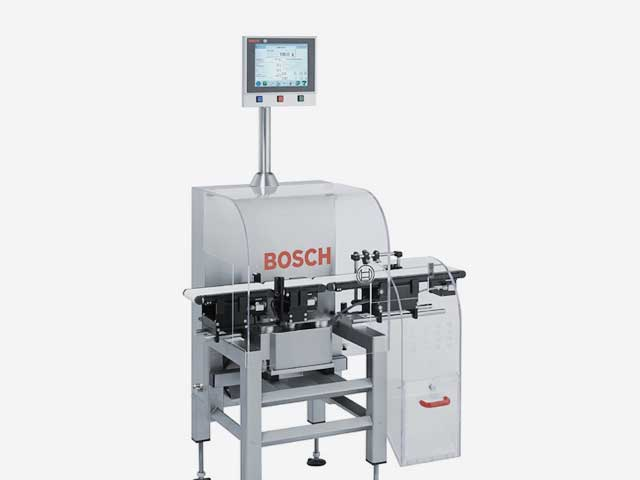
\includegraphics[scale=0.4]{images/kapitel_2/bosch_kwe.jpg}
    \caption{Abbildung einer Bosch KWE 4000}
    \label{fig:grundlagen_boschkwe}
\end{figure}

\section{Bosch Siegelmaschine}
Die Vertikale Form-, Füll- und Schließmaschine (kurz VFFS) ist für die Verpackung von  frei fließenden und losen
Lebensmittel, wie zum Beispiel Pulver, Proteine, Hähnchen sowie frische und gefrorene Produkte geeignet.

Dabei fallen die zu befüllenden Produkte vertikal aus dem oberen Bereich in den unteren Teil der Maschine. Dort baut
die Siegelmaschine den Behälter aus Folie zusammen, indem sie einen Schlauchbeutel formt und diesen versiegelt. Die
so geformten Beutel werden anschließend mit dem Produkt befüllt.

Der Behälter wird dann durch zwei Siegelbacken am oberen Ende verschlossen und ein Messer trennt ihn vom Rest des
Folienbandes ab. Der fertig befüllte Behälter fährt dann über ein Förderband aus der Maschine heraus und kann
weiterverarbeitet werden.

Das farbige Display dient zur Konfiguration der Maschine und kann die aktuelle Tätigkeit visualisieren. So können über
das Display alle Funktionen überwacht werden.

Die Abbildung~\ref{fig:grundlagen_boschvffs} auf Seite~\pageref{fig:grundlagen_boschvffs} zeigt eine Vertikale Form-,
Füll- und Schließmaschine mit ihrem gläsernen Befüllungsmodul und dem farbigen Display.

\begin{figure}[h]
    \centering
    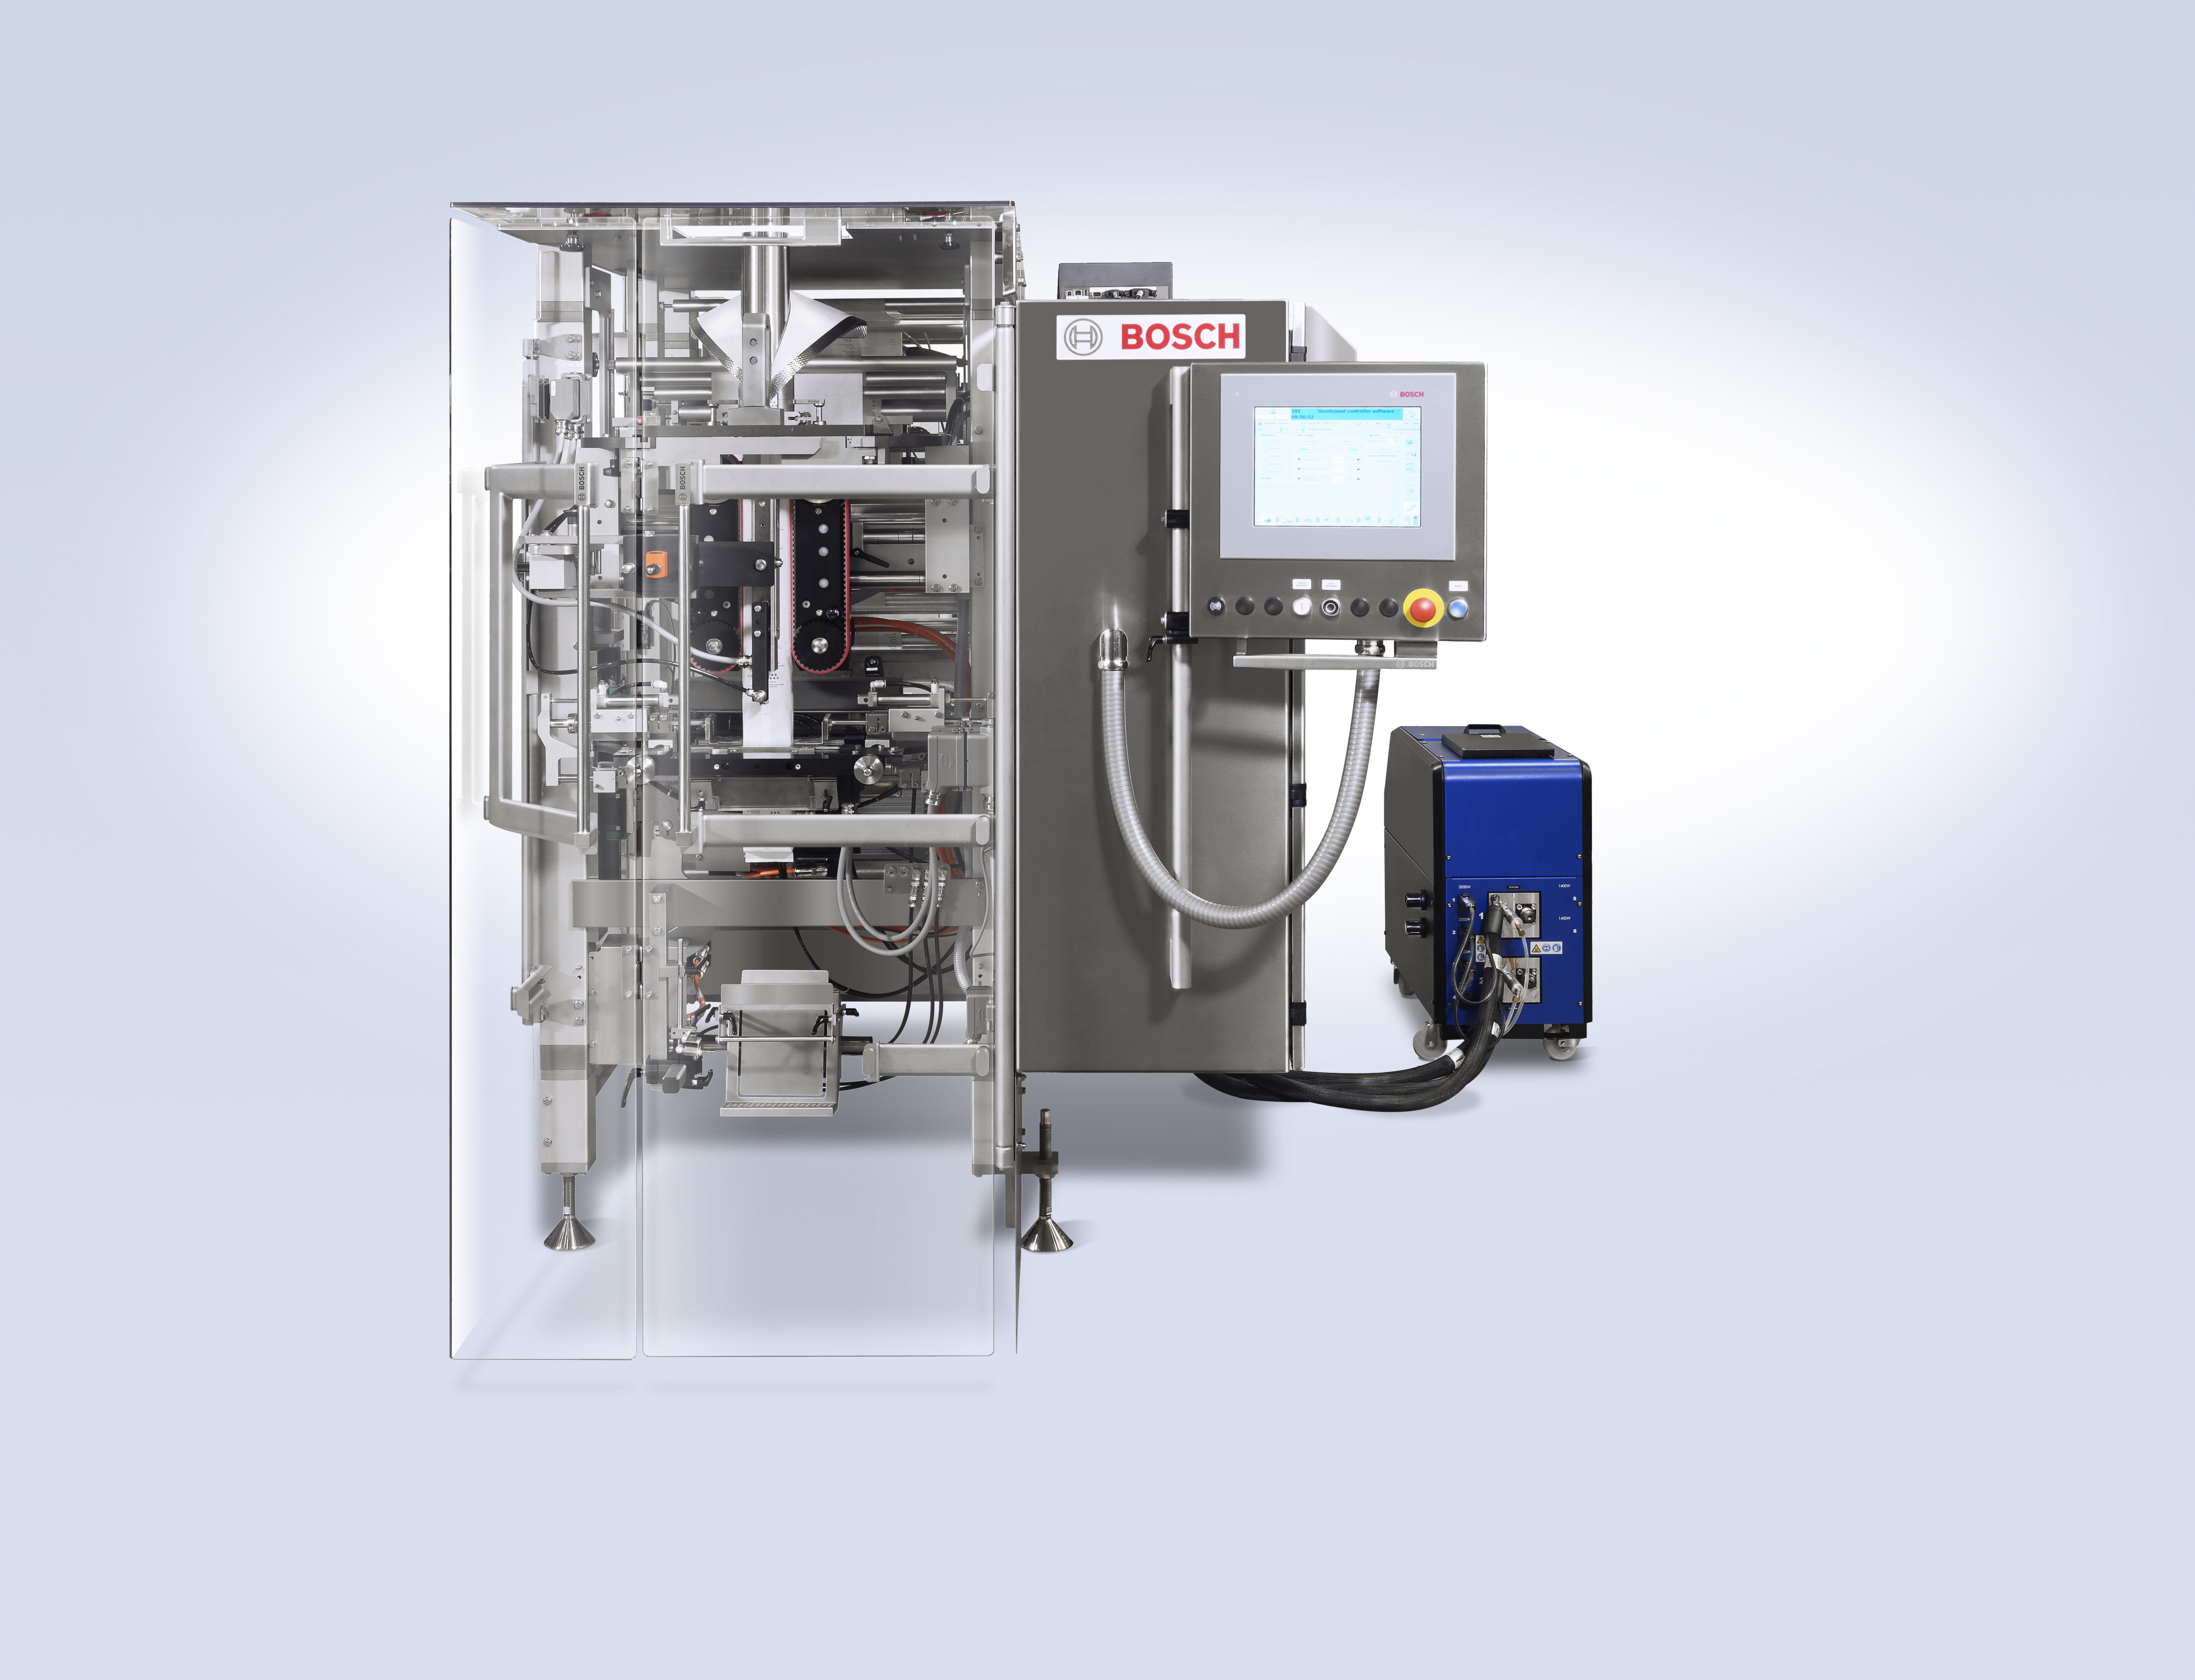
\includegraphics[scale=0.2]{images/kapitel_2/bosch_vffs.jpg}
    \caption{Abbildung einer Bosch VFFS}
    \label{fig:grundlagen_boschvffs}
\end{figure}

\section{Künstliche Intelligenz}
Künstliche Intelligenz (kurz KI) beziehungsweise Artificial Intelligence (kurz AI) ist ein Konzept für Maschinen, die
\enquote{wie Menschen denken} sollen. Dies umfasst das Lernen (die Erfassung von Informationen und Regeln für die
Verwendung der Informationen), die Schlussfolgerung (die Verwendung der Regeln, um ungefähre oder endgültige
Schlussfolgerungen zu ziehen) und die Selbstkorrektur.

Wie der KI Bundesverband e.V mitteilt, werden Maschinen in naher Zukunft noch nicht mit menschlicher Intelligenz
mithalten können. Allerdings wird sich KI auf viele Arten auf den Alltag auswirken, so der
Verein~\cite{article_grundlagen_ki}.

Die Künstliche Intelligenz kann auf verschiedene Arten kategorisiert werden. Folgend zwei stellvertretende Beispiele:

\begin{itemize}
    \item \textbf{Schwache KI} \\
    Die Schwache KI (englisch weak oder narrow AI) ist ein KI-System, das für eine bestimmte Aufgabe entwickelt und
    trainiert wird. Virtuelle persönliche Assistenten, wie der Google Assistant oder Alexa von Amazon, sind eine Form
    der schwachen KI.
    \item \textbf{Starke KI} \\
    Die starke KI (englisch strong AI) ist auch bekannt als die allgemeine künstliche Intelligenz. Sie simmuliert die
    menschlichen kognitiven Fähigkeiten und kann so noch unbekannte Aufgaben in der Zukunft lösen. Ein
    \textit{Turing Test} gibt darüber Auskunft, ob die Maschine eine starke KI besitzt.
\end{itemize}

Die Abbildung~\ref{fig:grundlagen_artificialintelligence} auf Seite~\pageref{fig:grundlagen_artificialintelligence} gibt
Auskunft über die Einteilung der Künstlichen Intelligenz in ihre Untergruppen. Dabei handelt es sich um eine eigene
Darstellung frei nach CodesOfInterest\footnote{https://codesofinterest.com/2016/11/difference-artificial-intelligence-machine-learning-deep-learning.html}.

\begin{figure}[h]
    \centering
    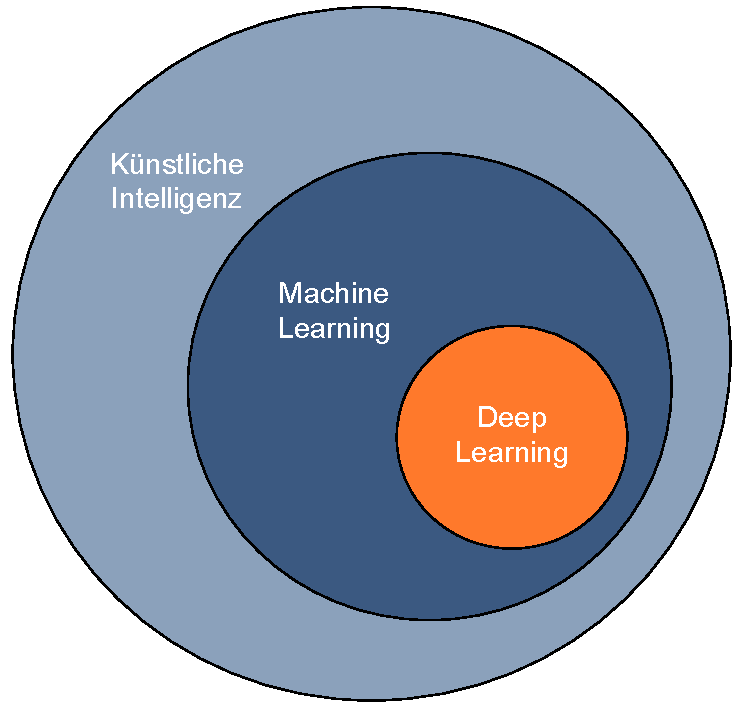
\includegraphics[scale=0.55]{images/kapitel_2/kuenstliche_intelligenz.pdf}
    \caption{Untergruppen der Künstlichen Intelligenz}
    \label{fig:grundlagen_artificialintelligence}
\end{figure}

Demnach ist \textit{Deep Learning} ein Teilbereich des \textit{Machine Learnings}, das wiederum ein Teilbereich der
\textit{Künstlichen Intelligenz} ist.

\section{Turing Test}
Der Naturwissenschaftler Alan Turing entwickelte 1950 den Turing Test. Dieser soll herausfinden, ob die Intelligenz eines
Systems der eines Menschen entspricht. Dieser Test wird regelmäßig zur Überprüfung und Einschätzung von Systemen
herangezogen.

Der Turing-Test basiert auf Konversation per Tastatur und Bildschirm, ohne jedoch Hör- und Sehkontakt zwischen den
Teilnehmern herzustellen. In dem Test sind zwei echte Personen (B und C) und die zu betestende Maschine involviert. Eine
Person (C) übernimme die Aufgabe eines Testers. Der Computer (A) und die verbleibende Person (B) bilden die kontrahenten.
Die Abbildung~\ref{fig:grundlagen_turingtest} auf Seite~\pageref{fig:grundlagen_turingtest} skizziert den Versuchsaufbau.

\begin{figure}[h]
    \centering
    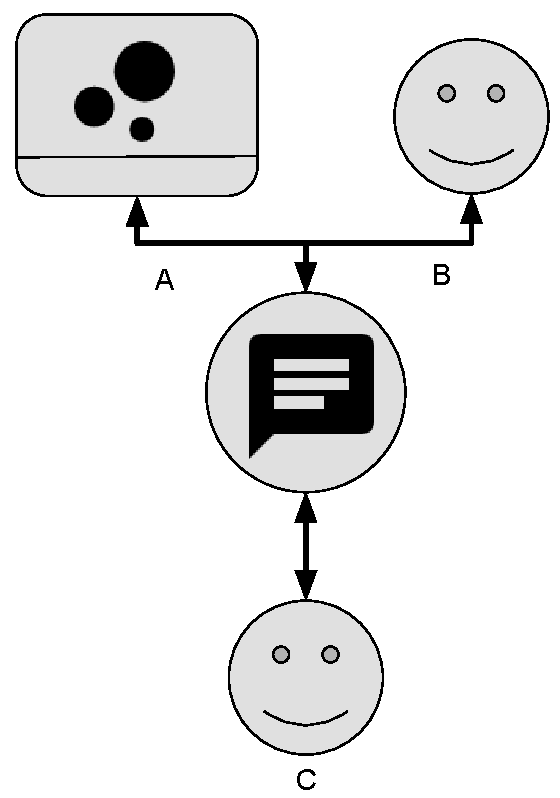
\includegraphics[scale=0.6]{images/kapitel_2/turing_test.pdf}
    \caption{Aufbau des Turing Tests}
    \label{fig:grundlagen_turingtest}
\end{figure}

Der Computer und die Person B versuchen ihren Gesprächspartner C in aufeinanderfolgenden Konversationen davon zu
überzeugen, dass sie der denkende Mensch sind. Sobald Person C nicht mehr zweifelsfrei bestätigen kann, welche Konversation
von der anderen Person und welche von der Maschine geführt wird, gilt der Test als bestanden (mehr
unter~\cite{online_grundlagen_turing}).

Jedoch ist dieser Test nicht frei von Kritik. Der Amerikanische Philosoph John Searle kritisiert zum Beispiel, dass mit
diesem Test lediglich die Funktionalität eines Systems überprüft wird, er jedoch nicht testet, ob die Maschine auch ein
Bewustsein oder eine Intentionalität hat.

Eine Maschine könnte diesen Test bestehen, wenn sie lediglich menschliches Verhalten imitiert und darauf programmiert
ist. Sie könnte den Tester so manipulieren, dass sie ihn für den echten Menschen hält.

%% TODO Umschreiben
\section{Machine Learning}
Machine Learning steht im Zentrum von KI und umfasst Algorithmen, mit denen Computer mit minimalem Programmieraufwand in
der Lage sind, aus Daten zu lernen.

Der Motor von KI ist eine Technologie namens "Machine Learning", die darauf ausgelegt ist, uns Arbeit abzunehmen und
produktiver zu machen.

%% TODO noch schreiben
\subsection{Algorithmen}
Welche Algorithmen gibt es dafür
\colorbox{yellow}{Hier fehlt was}

%% TODO noch schreiben
\subsection{Bewertungskriterien}
Welche Bewertungskreterien gibt es
\colorbox{yellow}{Hier fehlt was}

%% TODO noch schreiben
\subsection{Klassifikation}
Welche Klassifikationen gibt es
\colorbox{yellow}{Hier fehlt was}

%% TODO noch schreiben
\subsection{Neuronale Netze}
Was ist ein Neuronales Netz
\colorbox{yellow}{Hier fehlt was}

%% TODO noch schreiben
\section{Deep Learning}
Deep Learning ist eine KI-Methode, die mithilfe von komplexen Algorithmen Aufgaben in einem bestimmten Bereich
durchführt und diesen dabei mit geringer oder gänzlich ohne menschliche Überwachung erlernt. Kurzum: Computer lernen das
Lernen.
\colorbox{yellow}{Hier fehlt was}

\section{Cloud}
Für Cloud Computing hat sich die Kurzform Cloud etabliert. Dies versteht das Zusammenspiel von mehreren Servern in einem
Verbund. Diese Server übernehmen zum Beispiel Aufgaben wie etwa die Datenspeicherung oder komplizierte Programmabläufe.
Dabei ist für den Cloud-Nutzer nicht ersichtlich, wie viele Server in dieser Cloud stecken oder wo diese sich befinden.

Auch wenn ein Server in diesem Gesamtsystem ausfällt, hat dies keine Auswirkungen auf das gesamte System, da die Anfragen
und Aufgaben auf andere Systeme umgeleitet werden.

Durch NIST~\cite{online_grundlagen_cloud_nist} und~\cite{online_grundlagen_cloud_computing} zeichnet sich die Cloud durch
fünf wesentliche Eigenschaften aus:

\begin{itemize}
    \item \textbf{On-Demand Self Service} \\
    Registrierte Nutzer können Resourcen selbstständig instantiieren und konfigurieren.
    \item \textbf{Broad Network Access} \\
    Der Zugriff kann von verschiedenen Endgeräten erfolgen.
    \item \textbf{Resource Pooling} \\
    Alle Resourcen des Anbieters werden gebündelt und nach Bedarf den Nutzern zugewiesen.
    \item \textbf{Rapid Elasticity} \\
    Kapazitäten können nach Bedarf skaliert werden und stehen schnell und dynamisch zur Verfügung.
    \item \textbf{Measured Service} \\
    Es existiert eine automatische Kontrolle der Ressourcen durch einen Zähler, welcher die Transparenz für den
    Anbieter und den Benutzer ermöglicht.
\end{itemize}

Auf dem Markt existieren zahlreiche Cloud-Anbieter. Im folgenden wird auf drei der Top 10 größten Anbieter und deren
Lösungen im Bereich künstliche Intelligenz eingegangen (siehe hierzu~\cite{online_grundlagen_cloud}).

\subsection{Microsoft Azure}
Azure ist die Cloud-Computing-Plattform von Microsoft. Sie ist hoch skalierbar und wendet sich mit ihren Services
hauptsächlich an Unternehmen und Entwickler. Offiziell ist Azure seit 2010 verfügbar. Seitdem erscheinen in regelmäßigen
Abständen neue Services und Funktionen.

Nutzer der Plattform können Services aus den Bereichen Infrastructure as a Service (IaaS), Platform as a Service (PaaS)
und Software as a Service (SaaS) nutzen. Auch Datenbanken, Storagesysteme sowie virtuelle Maschinen, SQL-Datenbanken und
VPN-Gateways werden bereitgestellt.

Microsoft hat sich mit ihrer Platform Azure das Ziel gesetzt, Anwendern eine flexible Cloud-Infrastruktur zur Verfügung
zu stellen, die sich den individuellen Anforderungen schnell anpassen lässt und den Betrieb einer eigenen IT-Infrastruktur
überflüssig macht.

Dank weltweit betriebener Rechenzentren stehen die Dienste mit einer hohe Verfügbarkeit auf jedem Kontinent zur Verfügung.

Microsoft Azure ermöglicht den Einsatz von Hybrid-Systemen, bei denen nur ein Teil der Services in die Cloud verlagert
und der Rest auf lokalen Servern betrieben wird. Dienste von Drittanbietern bietet ein eigener Azure Marktplatz an
(mehr unter~\cite{online_grundlagen_azure}).

\subsubsection{Azure Machine Learning Studio}
Microsoft Azure Machine Learning Studio ist ein Tool mit dem Vorhersageanalysen erstellt, getestet und bereitgestellt
werden können. Dabei ist es für die Zusammenarbeit mittels Drag \& Drop konzipiert.

Die erstellten Modelle können als Webdiest zur Verfügung gestellt werden. Andere oder auch eigene Anwendungen können
diesen Webdienst mittels HTTP-Anfragen ansprechen und nutzen (siehe dazu~\cite{article_grundlagen_azure_studio}).

\subsection{Amazon Web Services}
AWS ist eine Tochterfirma von Amazon.com und bietet eine umfangreiche Plattform für Cloud-Computing-Services. Genau
wie in Microsoft Azure können dort Services für Infrastucture as a Service (IaaS), Platform as a Service (PaaS) und
Software as a Service (SaaS) genutzt werden.

Im Bereich IaaS haben Nutzer Zugrifff auf Datenspeicherung oder Rechenleistung. Über PaaS haben sie zugriff auf
Services zur einfachen Entwicklung von Webanwendungen. Bei SaaS existiert ein Katalog für Softwareanwendugnen von
externen Dienstleistern.

Ein bekanntes Beispiel für SaaS ist Google Docs, das eine standortunabhängige und Browserunabhängige Bearbeitung von
Dokumenten ermöglicht.

Public Clouds sind für Unternehmen nützlich, um beispielsweise schnell und einfach individuelle Anwendungen entwicklen
zu können ohne notwendige Produktlizenzen anderswo erwerben zu müssen.

AWS stellt Entwicklern eine maßgeschneiderte und zuverlässige IT-Infrastruktur auf Abruf zur Verfügung (= Self Service)
(mehr über AWS unter~\cite{online_grundlagen_aws}).

\subsubsection{Amazon Machine Learning}
Amazon Machine Learning ist ein Service innerhalb von AWS. Es bietet Visualisierungstools und Assistenten die den Aufbau
von Machine Learning-Modellen (ML) unterstützen, ohne dabei komplexe Algorithmen oder Technoligien vorauszusetzen.

Der Service nutzt leistungsstarke Algorithmen um ML-Modelle zu erstellen, indem er in den vorhandenen Daten automatisch
und selbstständig nach Mustern sucht. Anschließend werden diese Modelle dazu genutzt, um neue Daten zu verarbeiten und
Prognosen für eigene Anwendung zu generieren.

Der Service ist hochgradig Skalierbar und kann Milliarden Prognosen pro Tag generieren um diese in Echtzeit mit der
eigenen Anwendung zu teilen (mehr dazu in der Dokumentation~\cite{online_grundlagen_aws_learning}).

Nach dem Aufbau und dem Training der Modelle können diese über eine REST-API anderen Anwendungen zugänglich gemacht
werden, ohne sich dabei selbst um Infrastrukturen kümmern zu müssen.

\subsection{IBM Cloud (ehemals Bluemix)}
Die IBM Cloud (ehemals Bluemix genannt) ist die von IBM entwickelte Cloud Platform. In dieser sind mehr als 160 Services
inbegriffen um zum Beispiel mobile Apps oder Webanwendungen zu entwickeln. Weiter existieren zahlreiche Analysewerkzeuge
sowie Services von Drittanbietern.

Mit Watson Analytics lassen sich beispielsweise intelligente Systeme realisieren, die Daten kognitiv (also selbstlernend,
ohne für die Problemlösungen programmiert zu sein) auswerten und für die Entscheidungsfindung aufbereiten.

Die IBM Cloud unterstützt diverse schon integrierte DevOps-Dienste, um Cloud-Anwendungen zu erstellen, auszuführen,
bereitzustellen und zu verwalten. Die Platform basiert auf der Cloud Foundry Technologie und läuft auf IBMs
Softlayer Infrastruktur.

Sie unterstützt zahlreiche Programmiersprachen, einschließlich Java, Node.js, Go, PHP, Python, Ruby Sinatra, Ruby on
Rails und kann auch andere Sprachen wie Scala durch den Einsatz von Buildpacks unterstützen~\cite{book_grundlagen_bluemix}.

Weitere Informationen über Bluemix finden sich auf der Webseite\footnote{https://bluemix.net} und in der
Dokumentation\footnote{https://eu-gb.dataplatform.ibm.com/docs}.

\subsubsection{Watson Studio}
Watson Studio ist eine SaaS-Lösung der IBM Cloud und für die Erstellung, das Trainieren und das Verwalten von trainierten
Modellen zuständig. Diese Modelle werden, ähnlich denen von Microsoft Azure und AWS, über Drag \& Drop eingerichtet
und Versioniert.

Es bietet eine vielzahl von Anwendungen für die Verarbeitung von Daten und kann mit mehreren Endnutzern gleichzeitig
genutzt werden. In Watson Studio können Modelle erstellt, trainiert und verifiziert werden (mehr hierzu
unter~\cite{online_grundlagen_watson_studio}).

\subsubsection{Cloud Object Storage}
Der Service Cloud Object Storage ist für die Speicherung von unstrukturierten Daten in der Cloud zuständig. Dieser kann
sehr einfach erweitert werden um neuen Bedürfnissen zu genügen.

Die Architektur speichert und managed die Daten über Objekte. Dies hat einen großen Vorteil gegenüber der herkömmlichen
Speicherung über Blöcke und Volumes auf Festplatten. So finden sich alle Informationen, welche einen Datenstamm zugehörig
sind, an einer einzelnen Stelle. Diese Objekte können anschließend sehr einfach kopiert, erweitert oder entfernt werden.

Jedes Objekt hat eine globale und eindeutigen Identifierierung (ID) über die es gefunden werden kann. Außerdem enthält
ein Objekt Metadaten für eine Indezierung (mehr dazu unter~\cite{book_grundlagen_objectstorage}).

\subsubsection{Apache Spark}
Bei Apache Spark handelt es sich um ein Framework, welches unter der Open-Source-Lizenz verfügbar ist. Es ist ein Projekt
der Apache Software Foundation\footnote{https://www.apache.org} und entstand aus einem Forschungsprojekt der University
of California in Berkeley\footnote{https://www.berkeley.edu}.

Apache Spark ermöglicht es, Datenabfragen und große Datenmengen aus unterschiedlichen Quellen in hoher Geschwindigkeit
und guter Performance abzufragen und auszuführen. Dabei wird eine verteilte Architektur und Cluster Computing genutzt.

Viele große Unternehmen unterstützen die Weiterentwicklung von Apache Spark (mehr zu Apache Spark
unter~\cite{book_grundlagen_apachespark}).

\subsubsection{API Connect}
Mit dem Service IBM API Connect können alle vier Aspekte eines Application Programming Interfaces (kurz API)
Lebenszyklusses abgebildet werden: die Erstellung, die Ausführung, das Management und der Schutz einer eigenen API.

Mit diesem Services ist es möglich eine eigene API über ein Drag \& Drop Interface zu definieren und einzurichten. Die
so erstellten Schnittstellen können anschließend einfach über einen Webdienst zur Verfügung gestellt werden.

Dabei ist es möglich, verschienede Routen und Endpunkte zu definieren sowie die Schutzmaßnahmen und eventuelle
Zugangsverwaltung einzurichten (mehr in der Dokumentation~\cite{book_grundlagen_apiconnect}).

\subsubsection{Toolchain}
Bei einer Toolchain handelt es sich um ein Service zur Verwaltung von Entwicklung, Bereitstellung sowie Überwachung
einer Anwendung. Verschiedene Erweiterungen stehen nach der Einrichtung einer Toolchain zur Verfügung.

So ist es anschließend zum Beispiel möglich, eine Integration von einem vorhandenen GitHub-Projekt einzubauen oder eine
Verknüpfung mit einem Slack-Channel einzurichten, welche die wichtigsten Informationen der Toolchain automatisiert teilt.

Nachdem eine eingerichtete Toolchain mit einem Git-Repository verbunden wurde kann der Quelltext gebaut und auf einem
System installiert werden. Das Git-Repository kann entweder auf einem externen Service bereitstehen oder ein IBM internes
GitLab Projekt sein.

Bei der Toolchain handelt es sich unter anderem um ein \textit{Continuous Integration}-Tool (kurz CI)
(mehr über die Toolchain unter~\cite{online_grundlagen_toolchain}).

\section{TensorFlow.js}
TensorFlow ist eine Deep Learning Bibliothek welche von Google entwickelt wird. Die Bibliothek wird unter der freien
Apache 2.0 Lizenz vertrieben und ist sowohl unter allen gängigen Betriebssystemem lauffähig als auch bei den meisten
Cloud-Anbietern. Diese stellen entweder aktuelle Cloud Foundry-Container bereit oder eigene Python-Container.

TensorFlow ist der Nachfolger von Googles erstem Deep Learning Tool \textit{DistBelief}, welcher wiederum aus
\textit{Google Brain} hervorging. Ursprünglich wurde es zur Erkennung von Objekten auf Fotos und Videos entwickelt.

Die Berechnungen von neuronale Netzen können durch TensorFlow auf verteilte Computersysteme geschehen. Dies ist möglich,
da diese intern durch Graphen repräsentiert werden.

Aktuell wird TensorFlow für Predictive Analytics, Fraud Detection oder auch als Recommendation Engine bei Google und
vielen anderen Firmen verwendet.

In der neuesten Version lässt sich TensorFlow ohne großen Aufwand in Python integrieren. Dadurch können neue Lösungen
einfach zur Verfügung gestellt werden (mehr unter~\cite{book_grundlagen_tensorflow}).

Mittlerweile existiert eine mobile Lösung, die TensorFlow.js Bibliothek. Diese ist in jedem gängigen Browser oder auch
in Node.js lauffähig und macht schnelle \enquote{On the Edge}- sowie Offline-Vorhersagen möglich.

\section{Angular}
Bei Angular handelt es sich um ein von Google entwickeltes JavaScript-Framework. Es zielt auf die Entwicklung von
Web-Anwendungen ab und legt großen Wert auf Struktur und Qualität.

Mit seinem großen Fokus auf Architektur, Testing und isolierten Komponenten ist es für große Enterprise Anwendungen
bestens geeignet. Dabei war es das erste JavaScript-Framework das diesen Fokus hatte.

Durch Methoden wie Dependency Injection und ein ausgereiftes Tooling ermöglicht es effiziente und wartbare
Softwareentwicklung auf Basis von JavaScript (mehr unter~\cite{book_grundlagen_angular}).

\subsection{Model-View-Controller}
Die Programmarchitektur Model-View-Controller (kurz MVC) wurde um 1978 von Xerox entwickelt. Dabei wird eine
Anwendungskomponente in drei Teile zerlegt. In das oberflächenunabhängige \textit{Model}, das für die
Ausgabe zuständige \textit{View} und den für die Interpretation von Eingabeereignissen zuständigen \textit{Controller}.

Der Controller ist in dieser Architektur die Steuerungseinheit. Das Model beherbergt den Anwendungskern und die View
die Dargestellten Komponenten auf der Web-App.

Ein Controller zusammen mit einer View wird hier auch als eine Oberfläche bezeichnet. (mehr hierzu
unter~\cite{book_grundlagen_mvc}).

Es gibt zahlreiche Frameworks, welche das MVC-Patern umsetzen. Angular ist einer der bekanntesten Vertreter.

\subsection{Angular-Material}
Material Design ist eine von Google entwickelte Designsprache. Durch diese werden die Gestaltungsregeln des klassischen
Grafik-Designs mit den Möglichkeiten digitaler Benutzeroberflächen verbunden. Ziel ist es unter anderem die Verbesserung
von Benutzeroberflächen zu ermöglichen.

Material Design hat einen charakteristischen Look der es ermöglicht verschiedene Interfaces, welche im Material Design
gehalten sind, einfach zu kombinieren (mehr dazu in~\cite{online_grundlagen_materialdesign}).

Die JavaScript-Library \textit{Angular-Material} ermöglicht eine leichte integration des Material Designs in eine
Angular-Anwendung.

\subsection{ngx-restangular}
Mit der JavaScript-Library ngx-restangular können HTTP-Anfragen an REST-Schnitt\-stellen vereinfacht werden. Dabei
ermöglicht die Library vereinfacht Anfragen mittels den HTTP-Typen \textit{GET}, \textit{POST}, \textit{DELETE} und
\textit{UPDATE} zu stellen (mehr auf der betreffenden GitHub-Seite~\cite{online_grundlagen_restangular}).

Sie unterstützt in der Entwicklung und vereinfacht das Übergeben von Parametern an die Schnittstellen und die
Verarbeitung der Rückgabewerte.

\subsection{Observable}
Ein Observable ist das zentrale Konzept in Reactive Programming mit ReactiveX\footnote{http://reactivex.io}. Es
repräsentiert eine Menge von Daten, die in einer noch nicht bekannten Menge zu einem noch nicht bekannten Zeitpunkt
bereitstehen werden.

Ein Observer abonniert ein Observable und damit die später ankommenden Daten. Diese können gefiltert, gruppiert oder
transformiert werden. Auch Berechnungen sind mit den Daten möglich (mehr unter~\cite{book_grundlagen_observable}).

\subsection{Promise}
Bei Promises handelt es sich um eine Weiterentwicklung von Callbacks. Dabei helfen sie die Arbeit mit asynchronem Code
zu vereinfachen, indem sie asynchrone Operationen kapseln.

Sie zwängen asynchrone Operationen in eine einheitliche API, können verarbeitet werden bevor die Operation abgeschlossen
ist und es gibt zahlreiche Möglichkeiten Promises zu kombinieren oder in Sequenzen zu verwenden (mehr
in~\cite{book_grundlagen_promises} oder unter Matt Greer\footnote{http://www.mattgreer.org/articles/promises-in-wicked-detail}).

\subsection{flex-layout}
Bei flex-layout handelt es sich um ein Angular-Plugin, welches die Flexbox
CSS\footnote{https://www.w3schools.com/css/css3\_flexbox.asp}-Library für Angular implementiert.

Das Plugin hilft dabei, Webseiten auf verschiedene Browsergegebenheiten anzupassen. Dazu zählt unter anderem die Größe
des Displays oder die verwendete Version des Browsers.

Das Plugin hilft bei der Erstelltung von responsiven Webseiten indem es verschiedene Breakpoints zur Verfügung stellt
(mehr auf der GitHub-Page~\cite{online_grundlagen_flexlayout}).

\section{REST}
Representational State Transfer - Application Programming Interface (kurz REST-API) macht den Austausch von Informationen
über unterschiedliche Systeme möglich. Im Zeitalter verteilter Systeme und Cloud-Computing ist der Einsatz von REST-APIs
zur Kommunikation zwischen den Systemen notwendig.

Auch spricht man bei REST-APIs von Maschine-Maschine-Kommunikation, da die verschiedenen Systeme so eine gemeinsame
Sprache sprechen können um sich zu verständigen.

Mit der Hilfe von REST-APIs ist es möglich geworden, Informationen und Aufgaben auf verschiedene Systeme zu verteilen
(Microservices). Mit HTTP-Requests können Informationen dann verteilt werden. Jeder HTTP-Request setzt sich aus dem
Endpoint und den entsprechenden Parametern zusammen~\cite{online_grundlagen_rest}.

\section{Cloud Foundry}
Cloud Foundry ist eine Open Source Platform as a Service Lösung. Damit ist es für Entwickler möglich Anwendung zu bauen,
hochzuladen und auszuführen. Die nahezu grenzenlose Skalierbarkeit ist einer der größten Vorteile von Cloud
Foundry~\cite{book_grundlagen_cloudfoundry}.

Diese Skalierbarkeit wird durch die Container-Architektur erreicht. Jeder Container beinhaltet eine eigene
Anwendungsinstanz. Cloud Foundry unterstützt sowohl eine horizontale als auch eine vertikale Skalierung.

Bei der horizontalen Skalierung werden zusätzliche Container gestartet oder gestoppt. Ein Load Balancer kümmert sich um
die Verteiltung des Traffics. Bei der vertikalen Skalierung werden jeder Instanz individuell z.B. mehr oder weniger
Arbeitsspeicher oder CPU Zeit zugeteilt.

In der IBM Cloud erhält jede Cloud Foundry Instanz eine eigene IPV4-Adresse wodurch es mittels A-Record (Zuordnung eines
DNS-Namens zu IP-Adresse) möglich ist, eine eigene Domain mit der Anwendung zu verknüpfen.

\section{Version Control (Git)}
Git ist ein verteiltes Versionierungssystem, dass frei als Open-Source-Software zur Verfügung steht. Es wird bei der
Softwareentwicklung für die Versionskontrolle (stetige Protokollierung von Änderungen) von Dateien eingesetzt. (mehr
unter~\cite{book_grundlagen_git}).

\section{Node Package Manager (npm)}
Der Node Package Manager (kurz npm) ist ein Paketmanager für Node.js. Mit diesem lassen sich unter anderem
Software-Pakete für die Entwicklung von Projekten verwalten und steuern.

Es existiert eine Sammlung von Paketen (Repository) auf der offiziellen Webseite\footnote{https://www.npmjs.com}. Über
den entsprechenden Namen lassen sich die Pakete finden und im eigenen Projekt verwenden
(mehr unter~\cite{book_grundlagen_npm}).

\section{Mockups}
Ein Mockup findet seinen Einsatz bei der Planung von Webauftritten oder sonstigen Softwareprojekten welche eine grafische
Ausgabe besitzen. Mit diesen ist es möglich einen ersten Eindruck von der Gestaltung und den Funktionalitäten der
Anwendung zu bekommen. Ein großer Vorteil bei der Entwicklung von Mockups ist die Tatsache, dass kein Quellcode dafür
notwendig ist.

Mockups können auf dem Papier oder auch Computergestützt mit zahlreichen Programmen erstellt werden. Dazu zählt zum
Beispiel Balsamiq Mockups\footnote{https://balsamiq.com}.

Bei einem Mockup geht es darum, die verschiedenen Elemente einer Anwendung anzuordnen und einen optimalen Userflow
zu relaisieren. Das Design und etwaige Farben treten in den Hintergrund (mehr unter~\cite{book_grundlagen_mockups}).

\section{TypeScript}
Bei TypeScript (kurz TS) handelt es sich um ein Superset von JavaScript. Dies bedeutet, dass TypeScript ebenfalls eine
Implementierung von ECMAScript\footnote{https://en.wikipedia.org/wiki/ECMAScript} ist, JavaScript jedoch um zusätzliche
Features erweitert.

Jeder geschriebene JavaScript-Code funktioniert auch in TypeScript. Allerdings funktioniert nicht jeder TypeScript-Code
in JavaScript.

TypeScript erweitert JavaScript um mehrere Typings (und Annotations). Dies bedeutet, dass TypeScript, genau wie zum
Beispiel Java, Typensicher ist (mehr dazu unter~\cite{book_grundlagen_typescript}).

Im Listing~\ref{ls:grundlagen_typescript} auf Seite~\pageref{ls:grundlagen_typescript} ist ein originaler
JavaScript-Code in Zeile 2 zu sehen. In der Zeile 5 steht der entsprechende TypeScript-Code. Hier ist die
Typensicherheit gut zu erkennen.

\begin{lstlisting}[language=JavaScript, caption=Unterschied zwischen JavaScript und TypeScript, label=ls:grundlagen_typescript]
    // JavaScript
    var name = "Vorname Nachname";

    // TypeScript
    let name : string = "Vorname Nachname";
\end{lstlisting}

\section{WebView}
Ein WebView ist ein Android- oder iOS-Layout, welches Webseiten darstellen kann. Über diverse Schnittstellen werden dem
Layout Informationen wie Domain, Titel oder Größe übergeben. Das Layout kümmert sich anschließend selbstständig um das
Laden der entsprechenden Webseite und die Darstellung auf dem Bildschirm.

Das Layout steht sowohl unter Android als auch unter iOS seit den frühesten Versionen zur Verfügung (weitere
Informationen unter~\cite{online_grundlagen_webview}).
\chapter{Neuronales Netz}
\label{ch:neuronalesNetz}

Hier beschreiben, was im folgenden Kapitel gemacht werden soll? Was ist das Ziel? Was muss vorbereitet werden?
\\ \\
Ich habe Testdaten gesammelt und strukturiert. Ich habe ein neuronales Netz in der Cloud (Bluemix) aufgebaut und es
mit den gesammelten Daten trainiert und getestet. - Dann habe ich das Model deployed, damit man es per REST aufrufen kann.
- Dann damit rumprobiert. - Anschließend ein neuronales Netz mit Tensorflow aufgebaut und mit den gleichen Daten trainiert.
- Auch eine Schnittstelle gebaut, damit man die Funktion von außen aufrufen kann. - Am Schluss die Daten verglichen. Was
kommt bei der Cloud raus und was bei der Applikation - Bild mit schematischer Architektur (Markiert, was nun gemacht wird.
Rest ausgegraut)
\\ \\
1--2 Seiten
\section{Analyse}
Im folgenden sollen mehrere Ansätze für die Umsetzung des Neuronalen Netzes analysiert werden.

Wie könnte man das ganze umsetzen? Es gibt eigentlich zwei Möglichkeiten das umzusetzen.

\colorbox{yellow}{Hier fehlt was}

\subsection{Cloud}
Wir könnten es in der Cloud machen. Besprechen von Bluemix, Azure und AWS. Vor und auch Nachteile der Variante.

Azure kann kein Multi-Label Classification. Darum nur über Umwege (Selber schreiben oder Neuronale Netz an Neuronale Netz)
machbar.

\colorbox{yellow}{Hier fehlt was}

\subsection{Tensorflow}
Wie könnten es aber auch eigenständig mit Tensorflow machen. Vor und auch Nachteile der Variante. Vergleich Tensorflow
und TensorflowJS.

\colorbox{yellow}{Hier fehlt was}

\subsection{Hybrid}
Es wird eine Mischung aus den beiden Varianten. In der Cloud wird das Neuronale Netz aufgebaut und trainier -> Geschwindigkeit.
Dann kann es aber auch Deployed werden. Dann aber runterladen und mit TensorFlow.js einen Wrapper bauen um die gleiche
Datei/Modul.

\colorbox{yellow}{Hier fehlt was}
\section{Vorbereitung}
In diesem Kapitel werden Vorkehrungen für die Entwicklung eines Neuronalen Netzes und einer Tensorflow-Applikation
getroffen. Dafür muss zunächst ein kostenloses IBM Cloud Konto erstellt und drei Services eingerichtet werden.
Desweiteren werden zwei Programme auf dem Entwicklungsrechner installiert, die zur Entwicklung benötigt werden.

Im Weiteren werden die dafür notwendigen Schritte einzelnd erläutert.

\subsection{Bluemix Konto}
Um mit der IBM Cloud arbeiten zu können wird ein kostenloses Konto benötigt. Dies kann auf der
Registrierungsseite\footnote{https://console.bluemix.net/registration} erstellt werden.

Nach erfolgreicher Aktivierung des Kontos, mit einem an die hinterlegte E"=Mail"=Adresse verschickten Bestätigungslink,
kann das Konto 30 Tage lang ohne anfallende Gebühren für Services oder Runtimes genutzt werden.

Beim erstmaligen Aufruf des IBM Cloud Dashboards, wird nach einem Namen für die automatisch erstellte Organisation
gefragt. Dieser spielt für die Umsetzung keine Rolle und die Organisation kann zu jedem Zeitpunkt umbenannt oder auch
gelöscht werden. Ein Beispiel für den Organisationsnamen ist \texttt{Machine-Learning}.

Im Anschluss wird nach einem Namen für den ersten \texttt{Space} in der erstellten Organisation gefragt. Auch dieser
spielt für die Umsetzung keine Rollte und kann zu jedem Zeitpunkt umbenannt oder auch gelöscht werden. Ein Beispiel für
die Benamung des ersten Spaces ist \texttt{dev}, was eine Abkürzung für \textit{developper} ist.

In einem \texttt{Space} werden mehrere Runtimes und Services in einem Rechenzentrum gruppiert. Eine \texttt{Organisation}
kann mehrere Spaces beinhalten.

\subsection{IBM Cloud CLI}
Für die einfache Verwaltung der IBM Cloud empfiehlt es sich das zugehörige Command Line Interface (kurz \textit{CLI}) zu
installieren. Die Installation unter Linux und macOS erfolgt durch die Eingabe des folgenden Kommandos in eine Shell:

\begin{lstlisting}[language=bash, caption=Installation des IBM Cloud CLI, label=Installation des IBM Cloud CLI]
    $ curl -sL http://ibm.biz/idt-installer | bash
\end{lstlisting}

Anschließend kann die erfolgreiche Installation über das folgende Kommando überprüft werden:

\begin{lstlisting}[language=bash, caption=Installation des CLI überprüfen, label=Installation des CLI überprüfen]
    $ ibmcloud dev help
\end{lstlisting}

Die Ausgabe sollte eine Übersicht über alle möglichen Befehle des \textit{ibmcloud}-Tools geben. Sollte eine Fehlermeldung
erscheinen, hat die Installation nicht geklappt. Weitere Informationen gibt es auf der betreffenden
Installationsseite\footnote{https://console.bluemix.net/docs/cli/reference/bluemix\_cli/get\_started.html}.

Mit der Installation des IBM Cloud-CLI wird ein symbolischer Link über das Kommando \texttt{bx} angelegt. Somit kann der
Befehl \textit{ibmcloud} auch immer durch \textit{bx} ersetzt werden.

\subsection{Watson Studio}
Für den Aufbau und die Konfiguration des Neuronalen Netzes wird der Service \texttt{Watson Studio} benötigt. Aktuell gibt
es zwei Möglichkeiten einen Service oder eine Runtime in einen erstellten Space einzubinden.

\subsubsection*{Über das IBM Cloud Dashboard}
Auf dem IBM Cloud Dashbaord können mit einem Klick auf \texttt{Katalog} alle Services und Runtimes, welche aktuell genutzt
werden können, aufgelistet werden. In der Kategorie \texttt{Künstliche Intelligenz} kann der Service \texttt{Watson Studio}
ausgewählt werden.

Auf der sich öffnenden Seite kann der \textit{Servicename}, welcher frei gewählt werden kann, eingetragen werden.
Anschließend kann noch die Region, in welcher der Service zur Verfügung gestellt werden soll und die Ressourengruppe
definiert werden.

Mit einem Klick auf \texttt{Erstellen}, wird der Service Instanziiert und es erfolgt eine Weiterleitung zurück auf das
Dashbaord. Dort sollte der Service mit dem eingetragenen Name aufgelistet werden.

Auf dem Dashboard kann der Watson Studio Service durch einen Klick ausgewählt werden. Auf der folgenden Seite über die
Schaltfläche \texttt{Get Started} in das Watson Studio gewechselt werden.

\subsubsection*{Über die CLI}
Alternativ kann der Service mittels dem installierten CLI eingerichtet werden. Dazu muss das CLI mit dem IBM
Cloud-Konto verknüpft werden. Mittels dem folgenden Befehl wird der dafür nötige API-Endpunkt gesetzt:

\begin{lstlisting}[language=bash, caption=Setzen des API Targets, label=Setzen des API Targets]
    $ ibmcloud api https://api.ng.bluemix.net
\end{lstlisting}

Anschließend kann sich der Benutzer mit dem folgenden Befehl einloggen:

\begin{lstlisting}[language=bash, caption=Login über CLI und Single Sign-on, label=Login über CLI und SSO]
    $ ibmcloud login --sso
\end{lstlisting}

Der Parameter \texttt{sso} bewirkt, dass sich ein Browserfenster öffnet, das einen bequemen Login ohne Kommandozeile
ermöglicht.

Nach einem erfolgreichen Login, kann die genutzte Organisation ausgewählt werden. Dies geschieht über die Eingabe der
entsprechenden Nummer der Organisation. Der Login-Vogang ist damit abgeschlossen.

Im Weiteren kann ein \texttt{Watson Studio}-Service mit dem folgenden Befehl erstellt werden:

\begin{lstlisting}[language=bash, caption=Instanziierung des Watson Studio Services, label=Instanziierung des Watson Studio Services]
    $ ibmcloud cf create-service Watson-Studio lite sercive_name
\end{lstlisting}

Für den Parameter \texttt{service\_name} muss ein Name eingetragen werden, unter welchem der Service gefunden werden kann.
Über den Befehl \texttt{cf services} können alle instantiierten Services, welche sich in der vorher ausgewählten
Organisation befinden, aufgelistet werden.

\begin{lstlisting}[language=bash, caption=Auflisten aller Services, label=Auflisten aller Services]
    $ ibmcloud cf services
\end{lstlisting}

Der erstellte Service sollte mit dem eingegebenen Namen in der Liste aller Services erscheinen.

\subsection{API Connect}
\label{subsec:apiconnect}
\colorbox{yellow}{Hier fehlt was}

\subsection{Node.JS Runtime}
\label{ssc:nodejs_runtime}
Für die Erstellung der Node.JS-Applikation wird eine entsprechende Runtime in der IBM Cloud benötigt. Dafür wird ein
Cloud Foundry-Container mit Node.JS-"-Konfiguration erstellt. Dieser kann ebenfalls auf zwei unterschiedliche Weisen erstellt
werden.

Im vorangegangenen Kapitel wurden die zwei Varianten (über den IBM Cloud Katalog und über die Kommandozeile) ausführlich
erläutert. Im Folgenden wird lediglich die Erstellung über das CLI aufgezeigt:

\begin{lstlisting}[language=bash, caption=Instanziierung der Node.JS Runtime, label=Instanziierung der Node.JS Runtime]
    $ ibmcloud cf create-service nodejs service_name
\end{lstlisting}

Auch hier muss über den Parameter \texttt{service\_name} ein Name für die Applikation vergeben werden. Die URL, über die
der Container später aufrufbar ist folgt dem Schema \texttt{https://service\_name.mybluemix.net}.

\subsection{Git}
Für die Verwaltung und den späteren, automatisierten Installationsvorgang des Geschriebenen Quellcodes wird Git verwendet.
Das Programm kann unter Linux über das folgenden Kommando auf dem Entwicklnugsrechner installiert werden:

\begin{lstlisting}[language=bash, caption=Installation von Git, label=Installation von Git]
    $ sudo apt-get install git
\end{lstlisting}

Unter macOS steht ein grafische Installationsprogramm\footnote{http://sourceforge.net/projects/git-osx-installer} zur
Verfügung.

\subsection{Node.JS und npm}
Für die Entwicklung und die damit verbundenen Tests und Probeläufe auf dem Entwicklungsrechner wird ein installiertes Node.JS
benötigt. Die zur Zeit aktuellste LTS-Version (8.11.4) kann unter Linux wie folgt installiert werden:

\begin{lstlisting}[language=bash, caption=Installation von Node.JS, label=Installation von Node.JS]
    $ curl -sL https://deb.nodesource.com/setup_8.x | sudo -E bash -
    $ sudo apt-get install -y nodejs
\end{lstlisting}

Für macOS gibt es ein Installationspaket, welches auf der Download-Seite\footnote{https://nodejs.org/dist/v8.11.4/node-v8.11.4.pkg}
heruntergeladen werden kann.

Bei der Installation von Node.JS wir npm automatisch mitinstalliert. Dieser ist der Node.JS eigene Paketmanager und wird
für die spätere Installation von Abhängigkeiten für die Applikation benötigt.
\section{Umsetzung}
Wie die Zielarchitektur in Abbildung~\ref{fig:umsetzung_zielarchitektur} auf
Seite~\pageref{fig:umsetzung_zielarchitektur} zeigt, sollen Anfragen (englisch Requests) vom Frontend an die Anwendung
über den Service \textit{API Connect} laufen. Dieser Service verteilt die Anfragen anschließend auf zwei Systeme.

In einem System, \textit{Watson Studio}, erfolgt das Training für das neuronale Netz. Nach erfolgreichem Training wird es
als Modul in ein Deployment installiert. Dieses Deployment enthält eine REST-Schnittstelle, um Anfragen an das Model
bearbeiten zu können.

Das zweite System enthält einen \textit{Cloud Foundry Container}, welcher eine Node.js Runtime zur Verfügung stellt. Dieser
Container läuft in der Cloud und erhält eine IP sowie eine Domain über die er aufrufbar ist.

In der Runtime läuft eine \textit{TensorFlow.js} Applikation, welche das im Watson Studio trainierte Model enthält. Die
Applikation dient als Wrapper für das Model.

Im API Connect wird jeweils eine Route für das Watson Studio Deployment und eine für die TensorFlow.js Applikation
eingerichtet. So kann ein späteres System selbst entscheiden, welchen Endpunkt es für eine Vorhersage erreichen möchte.

In den folgenden Kapiteln wird die Architektur Schritt für Schritt umgesetzt, eingerichtet und die einzelnen Komponenten
überprüft.

\begin{figure}[h]
    \centering
    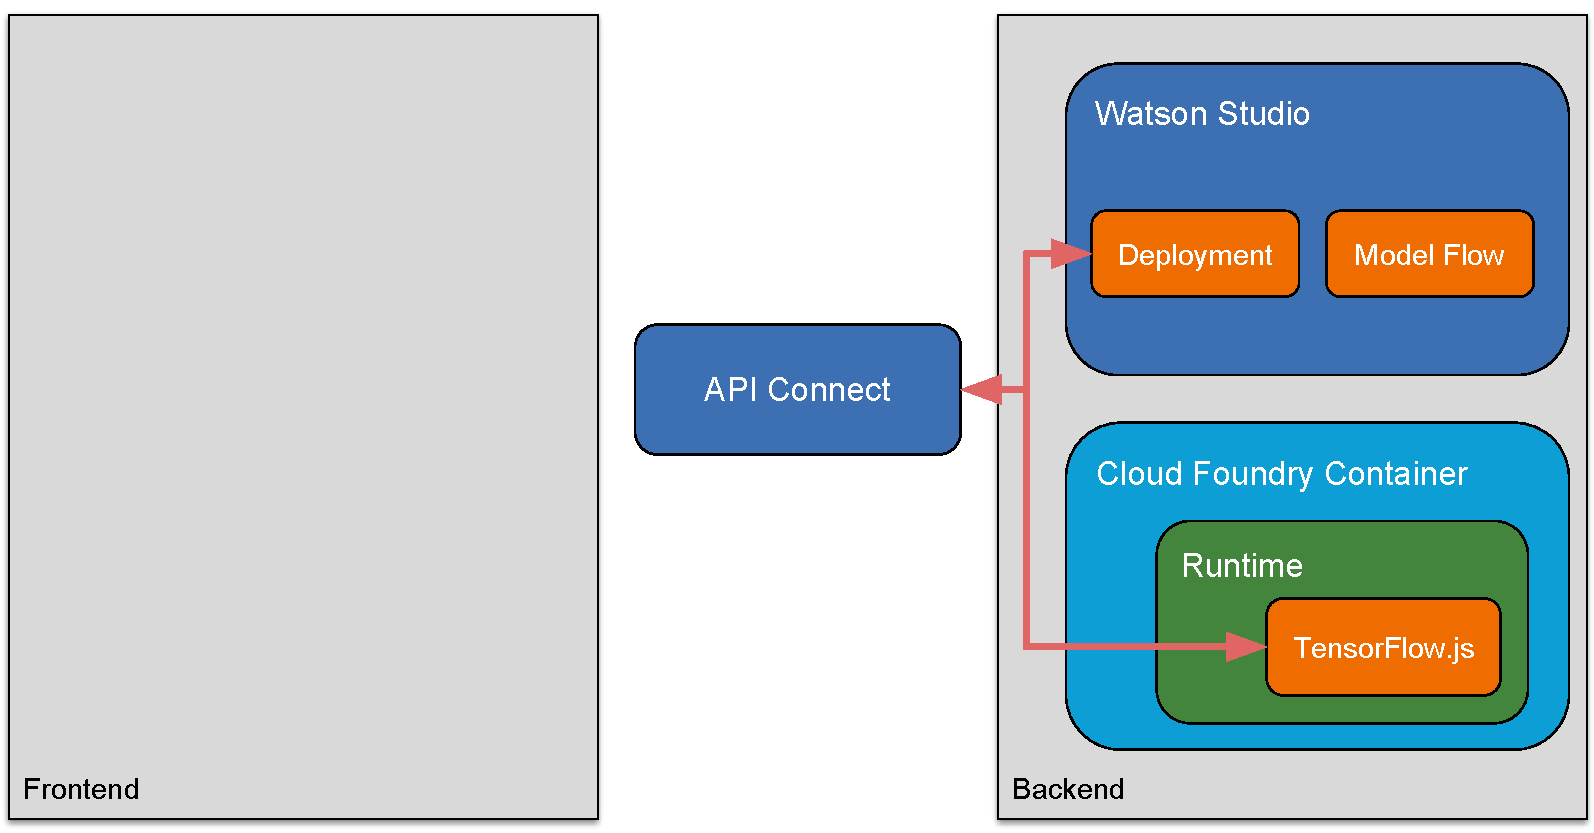
\includegraphics[width=\textwidth]{images/kapitel_3/architektur_uebersicht.pdf}
    \caption{Übersicht der Zielarchitektur}
    \label{fig:umsetzung_zielarchitektur}
\end{figure}

\subsection{Cloud}
Wie in der Vorbereitung, Kapitel~\ref{sec:analyse} auf Seite~\pageref{sec:analyse}, beschrieben, wird das neuronale Netz
in der Cloud erstellt, konfiguriert und trainiert. Wie bereits erwähnt hat dies einen enormen Geschwindigkeitsvorteil
gegenüber der offline trainierten Variante. Im Anschluss daran wird das trainierte Model heruntergeladen und mit einem
TensorFlow.js Wrapper nutzbar gemacht.

Die folgenden Kapitel beschreiben die notwendigen Schritte für die Erstellung eines neuronalen Netzes in der Cloud, das
trainierten des Models und das Einrichten eines Deployments für die REST-Schnittstelle.

\subsubsection{Daten zusammenstellen}
In einem ersten Schritt muss man die Daten, welche man später für das Training des neuronalen Netzes nutzen möchte,
sammeln und in einer Datei bündeln. Als Format eignet sich dafür eine Excel-Tabelle hervorragend, da das Anlegen der
Datensätze in Zeilen und Spalten sinnvoll ist.

Um eine Auswahl an Daten zu schaffen muss man sich darüber im klaren sein, welche Parameter existieren und welche Werte
durch das neuronale Netz vorhergesagt werden sollen. Auch ist wichtig zu wissen, welche Eingaben notwendig sind, um
überhaupt die Vorhersagen machen zu können.

In diesem Beispiel sollen Daten für das Bosch KWE Kontrollwaagensystem aufbereitet werden. Die vorhersagbaren Parameter
sind die, welche Angaben über den Pusher und über die Bandgeschwindigkeit zulassen.

Der Pusher wird durch insgesamt vier Parameter bestimmt. Die \textit{Druckluft} gibt darüber auskunft, wie stark oder
schnell der Pusher aus seiner Warteposition herausfährt. Der \textit{Impuls} gibt die Wucht an, mit der der Pusher
ausfährt.

Der Parameter \textit{Totzeit} gibt die Zeit an die gewartet wird, bis der Pusher herausfährt obwohl er schon das Signal
zum ausfahren bekommen hat. Über die \textit{Position} wird der Pusher auf der Waage positioniert. Die Angabe wird ab
dem Mittelpunkt der Wiegeeinheit gerechnet.

Für die Inputparameter, also die Parameter die später die Eingabevariablen des neuronalen Netzes sind werden alle die
genutzt, welche noch zur Verfügung stehen. Dabei handelt es sich um insgesamt 13 Stück. Sie sind in
Tabelle~\ref{tab:targets_inputs} auf Seite~\pageref{tab:targets_inputs} ersichtlich.

Alle Input-Werte sind in diesem Fall vom Kunden abhängig und desshalb problemlos Recherchierbar beziehungsweise abgelegt
und gespeichert.

In der noch leeren Excel-Tabelle muss man nun in den Spalten die Eingabeparameter aber auch die vorhersagbaren Parameter
auflisten. Jede leere Zeile wird durch ein Produkt ersetze. So listet man alle historischen Daten untereinander auf und
befüllt jede Spalte mit den entsprechenden Informationen.

Sollte man für eine Spalte keinen Wert haben, so muss die Zeile leer gelassen und es darf keine null oder sonstiges
eingetragen werden.

In Anhang~\ref{sec:scaleData} auf Seite~\pageref{sec:scaleData} sind die Beispieldaten für die Waage aufgezeigt. Die
folgenden Kapitel beziehen sich auf diesen Datensatz.

Da die Daten zusammengestellt sind, kann man sie in einem weiteren Schritt in das Watson Studio importieren um das
neuronale Netz zu trainieren.

\subsubsection{Daten importieren}
Nachdem man die Trainingsdaten zusammengestellt hat, kann man diese nun in das Watson Studio importieren. Dazu existiert
im Watson Studio Dashboard ein Menüpunkt mit dem Namen \textit{Assets} am oberen Menüband.

Dieser beinhaltet alle hochgeladenen, generierten oder gesammelten Daten, Modelle, Dashboards, Notebooks oder Flows. Die
oberste Kategorie, \textit{Data Assets}, listet alle Trainingsdaten in Form von Excel-Tabellen für die Weiterverarbeitung
auf. In diese Kategorie muss man die zuvor erstellte Tabelle hochladen.

Über den Menüpunkt \texttt{New data asset} kann man die erstellte Datei hochladen. Ein Klick auf diesen Menüpunkt öffnet
einen seitlichen Arbeitsbereich. Der Nutzer kann über den Menüpunkt \texttt{Browse} die Dateiauswahl des Betriebssystems
öffnen und seine Datei auswählen. Bei der Auswahl handelt es sich um die im vorangegangenen Kapitel erstellte Datei mit
Trainingsdaten.

Alternativ kann man die Datei auch in das fabrlich hervorgehobene Feld schieben. Der Upload der Datei startet damit
sofort.

Nach wenigen Sekunden ist die Datei hochgeladen und wird im Bereich \textit{Data assets} angezeigt. Damit ist der
Uploadvorgang erfolgreich abgeschlossen und die Datei kann im nächsten Schritt umgewandelt werden.

\subsubsection{Daten umwandeln}
Da die erstellte Datei mit den Trainigsdaten nun in Watson Studio bereitsteht, ist die Umwandlung in eine CSV-Datei
möglich. Dieser Schritt ist zwingend notwendig, damit die Datei später als Eingabeparameter für das neuronale Netz
dienen kann. Ein anderes Format wird als Eingabe zur Zeit nicht unterstützt.

In Watson Studio liegt mit den \textit{Data flows} ein einfaches Werkzeug bereit, um Dateien in das benötigte CSV-Format
zu überführen. Dazu kann der Nutzer in der Kategorie Data Flows über \texttt{New data flow} ein neuer Flow anlegen.

Im folgenden öffnet sich der Wizzard zum Erstellen des Flows. Der Nutzer muss im linken Bereich die umzuwandelnde Datei
auswählen. Dabei handelt es sich um die hochgeladene Datei. Über die Schaltfläche \texttt{Add} kann man die Auswahl
übernehmen.

Nun ist der Inhalt der Datei im mittleren Bereich des Displays sichtbar. Bei dieser Ansicht ist darauf zu achten, dass
die Interpretation der Werte der einzelnen Spalten als Dezimal-Zahl erfolgt. Diese Information steht unterhalb der
einzelnen Spaltenüberschriften. Sollte diese Einstellung nicht voreingestellt sein, muss man diese manuell abändern.

Dazu klickt man in der entsprechenden Spalte oben, rechts neben dem Spaltenname, auf die drei Punkte (Einstellungen) und
selektiert den Eintrag \texttt{Convert Column}. Im Untermenü muss man dann den Wert \texttt{Decimal} bestätigen. Nun
werden die Zahlen in der Spalte auch korrekt als Dezimal-Zahl interpretiert.

Da es sich bei allen Zahlen nun um Dezimal-Zahlen handelt, kann man über die Schaltfläche \texttt{Run data flow} die
Konvertierung starten. Bevor die Konvertierung jedoch startet, zeigt das System eine Übersicht über die einzelnen
Schritte, die dazu benötigt werden, an.

Hier werden zum Beispiel etwaige Konvertierungen zu Dezimal-Zahlen angezeigt oder sonstige Operationen dargestellt. Da
es sich hierbei lediglich um Informationen handelt, kann der Nutzer die Seite bestätigen und der Flow startet.

Nach wenigen Minuten sollte im Watson Studio im Bereich Assets, in der Kategorie Data Assets, die neue Datei zur
Verfügung stehen. Dabei trägt die Datei die Dateiendung \textit{.csv}. Die Konvertierung der Datei ist somit
abgeschlossen und man kann sie für das neuronale Netz verwenden.

\subsubsection{Modeler Flow}
\label{subsub:modeler_flow}
Nach erfolgreicher Konvertierung der Trainingsdaten kann man diese für das neuronale Netz nutzen. Für die Erstellung
des neuronalen Netzes und den damit verbundenen Parameterübergaben für die Vorhersage ist der \texttt{Modeler Flow} am
Besten geeignet.

Über die Schaltfläche \texttt{New Flow} im Bereich Assets erstellt man diesen und richtet ihn ein. Nachdem man einen Namen
und eine optionale Beschreibung für den Flow eingegeben hat, muss man die Auswahl \textit{Modeler Flow} und
\textit{IBM SPSS Modeler} auswählen. Dabei handelt es sich um den Standard-Flow von Watson Studio.

Der Nutzer bestätigt die Eingabe über die Schaltfläche \texttt{Create} und nach kurzer Zeit ist der Flow erstellt und es
erscheint ein leerer Arbeitsbereich im Browser.

Der Menüpunkt \texttt{Palette} zeigt einen linken Arbeitsbereich mit allen aktuell verfügbaren Modulen, gruppiert an. In
diesem muss man den Baustein \textit{Data asset} in der Gruppe \textit{Import} auswählen.

Dieser Baustein ermöglicht den Import der konvertierten Trainingsdaten für das neuronale Netz. Über Drag \& Drop kann der
Nutzer den Baustein in den noch leeren Arbeitsbereich platzieren.

Um den Baustein zu konfigurieren Klickt der Entwickler doppelt auf den Baustein. Daraufhin öffnet sich ein rechter,
seitlicher Arbeitsbereich. In diesem kann er über die Schaltfläche \texttt{Change Data Asset} die Datei auswählen, welche
die Trainingsdatensätze enthält.

In dieser Liste steht lediglich die vorher erstellte CSV-Datei zur Verfügung, da bisher lediglich CSV-Dateien als
Eingabeparameter genutzt werden können. Über \texttt{Save} wird die Einstellung gespeichert und der Baustein ist fertig
konfiguriert.

Im nächsten Schritt erfolgt die Konfiguration des neuronalen Netzes. Dazu existiert in der Kategorie \textit{Modeling}
das Modul \textit{Neural Net}. Das stellt für den Anwendungsfall die beste Alternative dar, da es sich hierbei um ein
allgemeines neuronales Netz handelt. Dies kann allerdings sehr tief konfiguriert werden.

Genau wie das Import-Modul kann man dieses mit der Maus in einen freien Bereich des Arbeitsbereiches platzieren. Somit
ist das Modul Teil des Prozesses und der Entwickler kann es konfigurieren.

Damit das neuronale Netz die importierten Datensätze nutzen kann, wird eine Verbindung zwischen dem \textit{Import-Modul}
und dem \textit{Neural-Net-Modul} aufgebaut. Mit einen Klick auf den Ausgang des Import-Moduls startet man eine
Verbindungslinie.

Mit einem anschließenden Klick auf den Eingang des Neural-Net-Modul kann man die Verbindung fertig aufbauen. Die Verbindung
wird nun über eine durchgezogene Linie zwischen den beiden Modulen visualisiert.

Bei einer Verbindung wird der Output eines Modules an das mit einer visualisierten Linie verbundenen Modul weitergegeben.
Dieses Folgemodul kann die Werte dann als Eingabevariablen nutzen. Einen Ausgang kann man mit mehreren Eingängen
verbinden. Dabei stehen dann allen weiteren Modulen die gleichen Werte zur Verfügung.

Die Konfiguration des Neural-Net-Moduls erfolgt durch einen doppelten Klick auf dieses. Damit man die
\textit{Targets} und die \textit{Inputs} selbst definieren kann, muss man den Hacken bei \enquote{Use custom field roles}
setzen. Andernfalls versucht Watson selbst die Inputs und die Outputs zu definieren. Meist sind diese Einstellungen dann
aber falsch.

Die Tabelle~\ref{tab:targets_inputs} auf Seite~\pageref{tab:targets_inputs} zeigt die auszuwählenden Tabellenspalten für
die jeweilige Kategorie. Die Targets beschreiben die Variablen, welche durch den Watson Service Vorhergesagt werden
sollen. Die Inputs definieren die Größen, durch welche eine Vorhersage überhaupt möglich ist.

Dem resultierenden, trainierten Model werden zu einem späteren Zeitpunkt die Inputs übergeben und die Targets kommen als
vorhergesagte Rückgabeparameter zurück.

\begin{table}[h]
    \centering
    \begin{tabular}{|c|c|}
        \hline
        \textbf{Targets} & \textbf{Inputs}\\
        \hline
        \hline
        Leistung & Einlaufbandlänge\\
        \hline
        Druckluft & Wägebandlänge\\
        \hline
        Impuls & Auslaufbandlänge\\
        \hline
        Totzeit & Einlaufbandbreite\\
        \hline
        Position & Wägebandbreite\\
        \hline
        & Auslaufbandbreite\\
        \hline
        & Einlaufbandrolle\\
        \hline
        & Wägebandrolle\\
        \hline
        & Auslaufbandrolle\\
        \hline
        & Produktbreite\\
        \hline
        & Produktlänge\\
        \hline
        & Produkthöhe\\
        \hline
        & Packungsgewicht\\
        \hline
    \end{tabular}
    \caption{Variablen für die Targets und die Inputs}
    \label{tab:targets_inputs}
\end{table}

Mit dieser Konfiguration werden 13 Parameter als Eingabevariablen genutzt und fünf Parameter durch das neuronale Netz
vorhergesagt.

Vier der vorhergesagten Parameter (Druckluft, Impuls, Totzeit und Position) beziehen sich auf den \textit{Pusher} und
der Parameter \textit{Leistung} gibt die tatsächliche Bandgeschwindigkeit an, mit der das Band in der Maschine laufen
soll.

Alle anderen Einstellungen des neuronalen Netzes werden im ersten Schritt auf den Standardeinstellungen belassen. Zu
einem späteren Zeitpunkt, wenn sich Testdaten ändern oder Parameter angepasst werden müssen, kann man mit den weiteren
Einstellungen das neuronale Netz anpassen und gegebenenfalls optimieren.

Der Flow für das neuronale Netz ist somit fertiggestellt. Mit einem Klick auf \texttt{Run} startet das Training des
neuronalen Netzes.

Nach dem erfolgreichem Training des neuronalen Netzes erscheint das trainierte Model unterhalb des neuronalen Netzes im
aktuellen Arbeitsbereich. Eine gestrichelte Linie zwischen dem neuronalen Netz und dem trainierten Model zeigt die
Abhängigkeit der beiden Module an.

Für die Weiterverarbeitung und ein späteres Deployment des trainierten Models muss man dieses mit einem Export-Modul
verbinden. Der Export erfolgt über das Modul \textit{Table}.

Das Table-Modul befindet sich in der Kategorie \textit{Outputs} und wird, genau wie alle andere Module, frei auf dem
Arbeitsbereich platziert. Eine Verbindung zwischen dem trainierten Model und der Table ermöglicht den Datenaustausch.
Für die Table ist keine weitere Konfiguration notwendig.

Ein Rechtsklick auf das Table-Modul öffnet das Kontextmenü des Moduls. Darüber lässt sich der Punkt
\enquote{Save branch as a model} anklicken. Dieser ermöglicht es, das trainierte Model zu exportieren.

In dem sich öffnenden Fenster muss man den Namen und eine optinale Beschreibung für das neue Model definieren. Mit einem
Klick auf den Button \texttt{Save} wird das Model gespeichert und es erscheint im Watson Studio Dashboard.

In der Abbildung~\ref{fig:umsetzung_model_flow} auf Seite~\pageref{fig:umsetzung_model_flow} ist der vollständige Aufbau
des Model Flows dargestellt mit seinem trainierten Model und der Tabellen-Exportierung.

\begin{figure}[h]
    \centering
    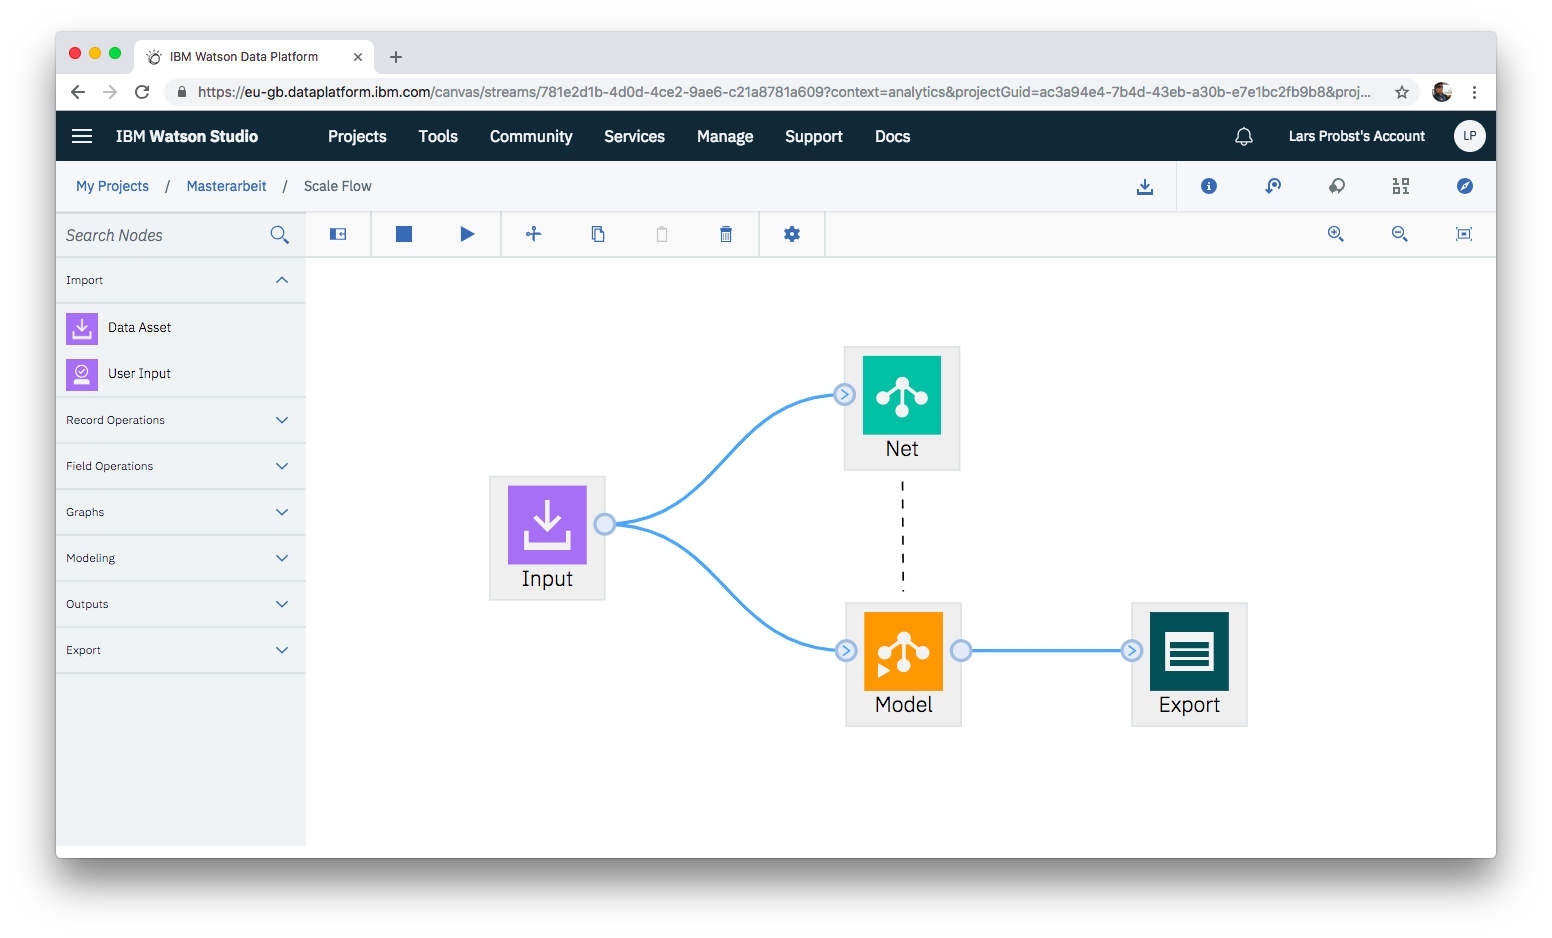
\includegraphics[width=\textwidth]{images/kapitel_3/umsetzung_model_flow.png}
    \caption{Vollständiger Model Flow}
    \label{fig:umsetzung_model_flow}
\end{figure}

\subsubsection{Informationen zum Model}
Über einen weiteren Rechtsklick auf das trainierte Model kann man über den Menüpunkt \texttt{View Model} auf eine
detaillierte Übersicht des Models gelangen. Hier finden sich zahlreiche Informationen, die unter anderem Aufschluss
über die Genauigkeit des Models geben.

Die erste Information, welche man als Benutzer über das Model zu sehen bekommt, ist in
Abbildung~\ref{fig:umsetzung_model_evaluation} auf Seite~\pageref{fig:umsetzung_model_evaluation} zu sehen \textendash{}
die \texttt{Evaluation}.

\begin{figure}[h]
    \centering
    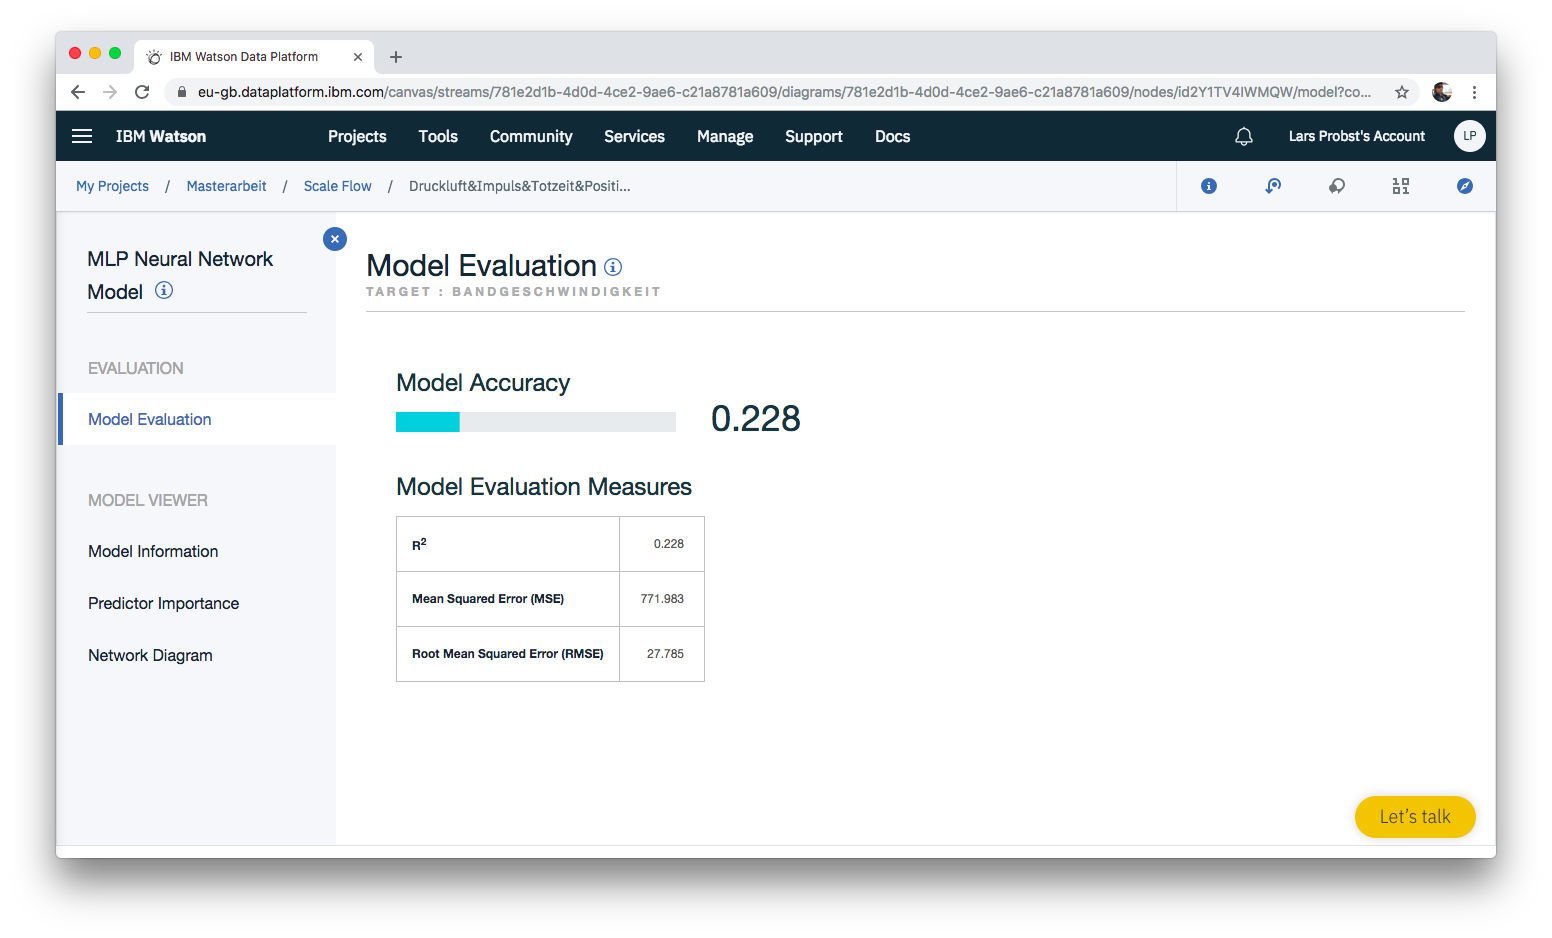
\includegraphics[width=\textwidth]{images/kapitel_3/model_evaluation.png}
    \caption{Evaluation des trainierten Models}
    \label{fig:umsetzung_model_evaluation}
\end{figure}

Die große Zahl gibt die tatsächliche Genauigkeit des Models (englisch Model Accuracy) an. Mit 100 multipliziert, erhält
man die prozentuale Angabe der Genauigkeit. Wenn man mit dem Mauszeiger über die Zahl fährt, erhält man eine genauere
Angabe mit Nachkommastellen.

Die Genauigkeit berechnet sich durch ein Testdatenset, welches dem Trainingsdatenset automatisch entnommen wird. Dabei
kann beim trainieren des Models angegeben werden, um wie viele Datenset es sich handeln soll.

Nachdem das Model fertig trainiert ist, wird es mit den zur Verfügung stehenden Testdaten gefüttert. Im Anschluss werden
die vorhergesagten Werte mit denen im Testdatenset verglichen. Je größer die Abweichung ist, desto geringer ist die
Genauigkeit des trainierten Models.

Im Weiteren finden sich Bewertungskriterien für das trainierte Model (englisch Model Evaluation Measures). Diese geben
Aufschluss darüber, wie gut das Model ist. In der ersten Zeile wird zum Beispiel $\mathbf{R^2}$ ausgegeben.  Dabei
handelt es sich um den Determinationskoeffizient. Dieser ist eine wichtige Kennzahl zur formalen Beurteilung der
Regression. Weitere Informationen sind auf der Wikipedia-Seite\footnote{https://de.wikipedia.org/wiki/Bestimmtheitsmaß}
ersichtlich.

Der nächste Wert entspricht der \enquote{Mittleren quadratische Abweichung} (englisch Mean Squared Error). Dies ist der
Durchschnitt der quadrierten Fehler. Als Fehler ist die Differenz der vorhergesagten Werte und der tatsächlichen Werte
definiert.

Der letzte Wert gibt das \enquote{Mittleres Abweichungsquadrat} (englisch Root Mean Squared Error) an. Dieser Wert ist
ein Maß für die Unterschiede zwischen Werten, die von einem Modell vorhergesagt werden, und den tatsächlich beobachteten
Werten.

In der nächsten Kategorie, Model Viewer, sind Informationen zu den einzelnen Werten des neuronalen Netzes angegeben.
Im ersten Menüpunkt, Model Information, stehen alle generellen Informationen.

Mit einem Klick auf den Menüpunkt gelangt man in eine Ansicht wie in Abbildung~\ref{fig:umsetzung_model_information}
auf Seite~\pageref{fig:umsetzung_model_information} zu sehen.

\begin{figure}[h]
    \centering
    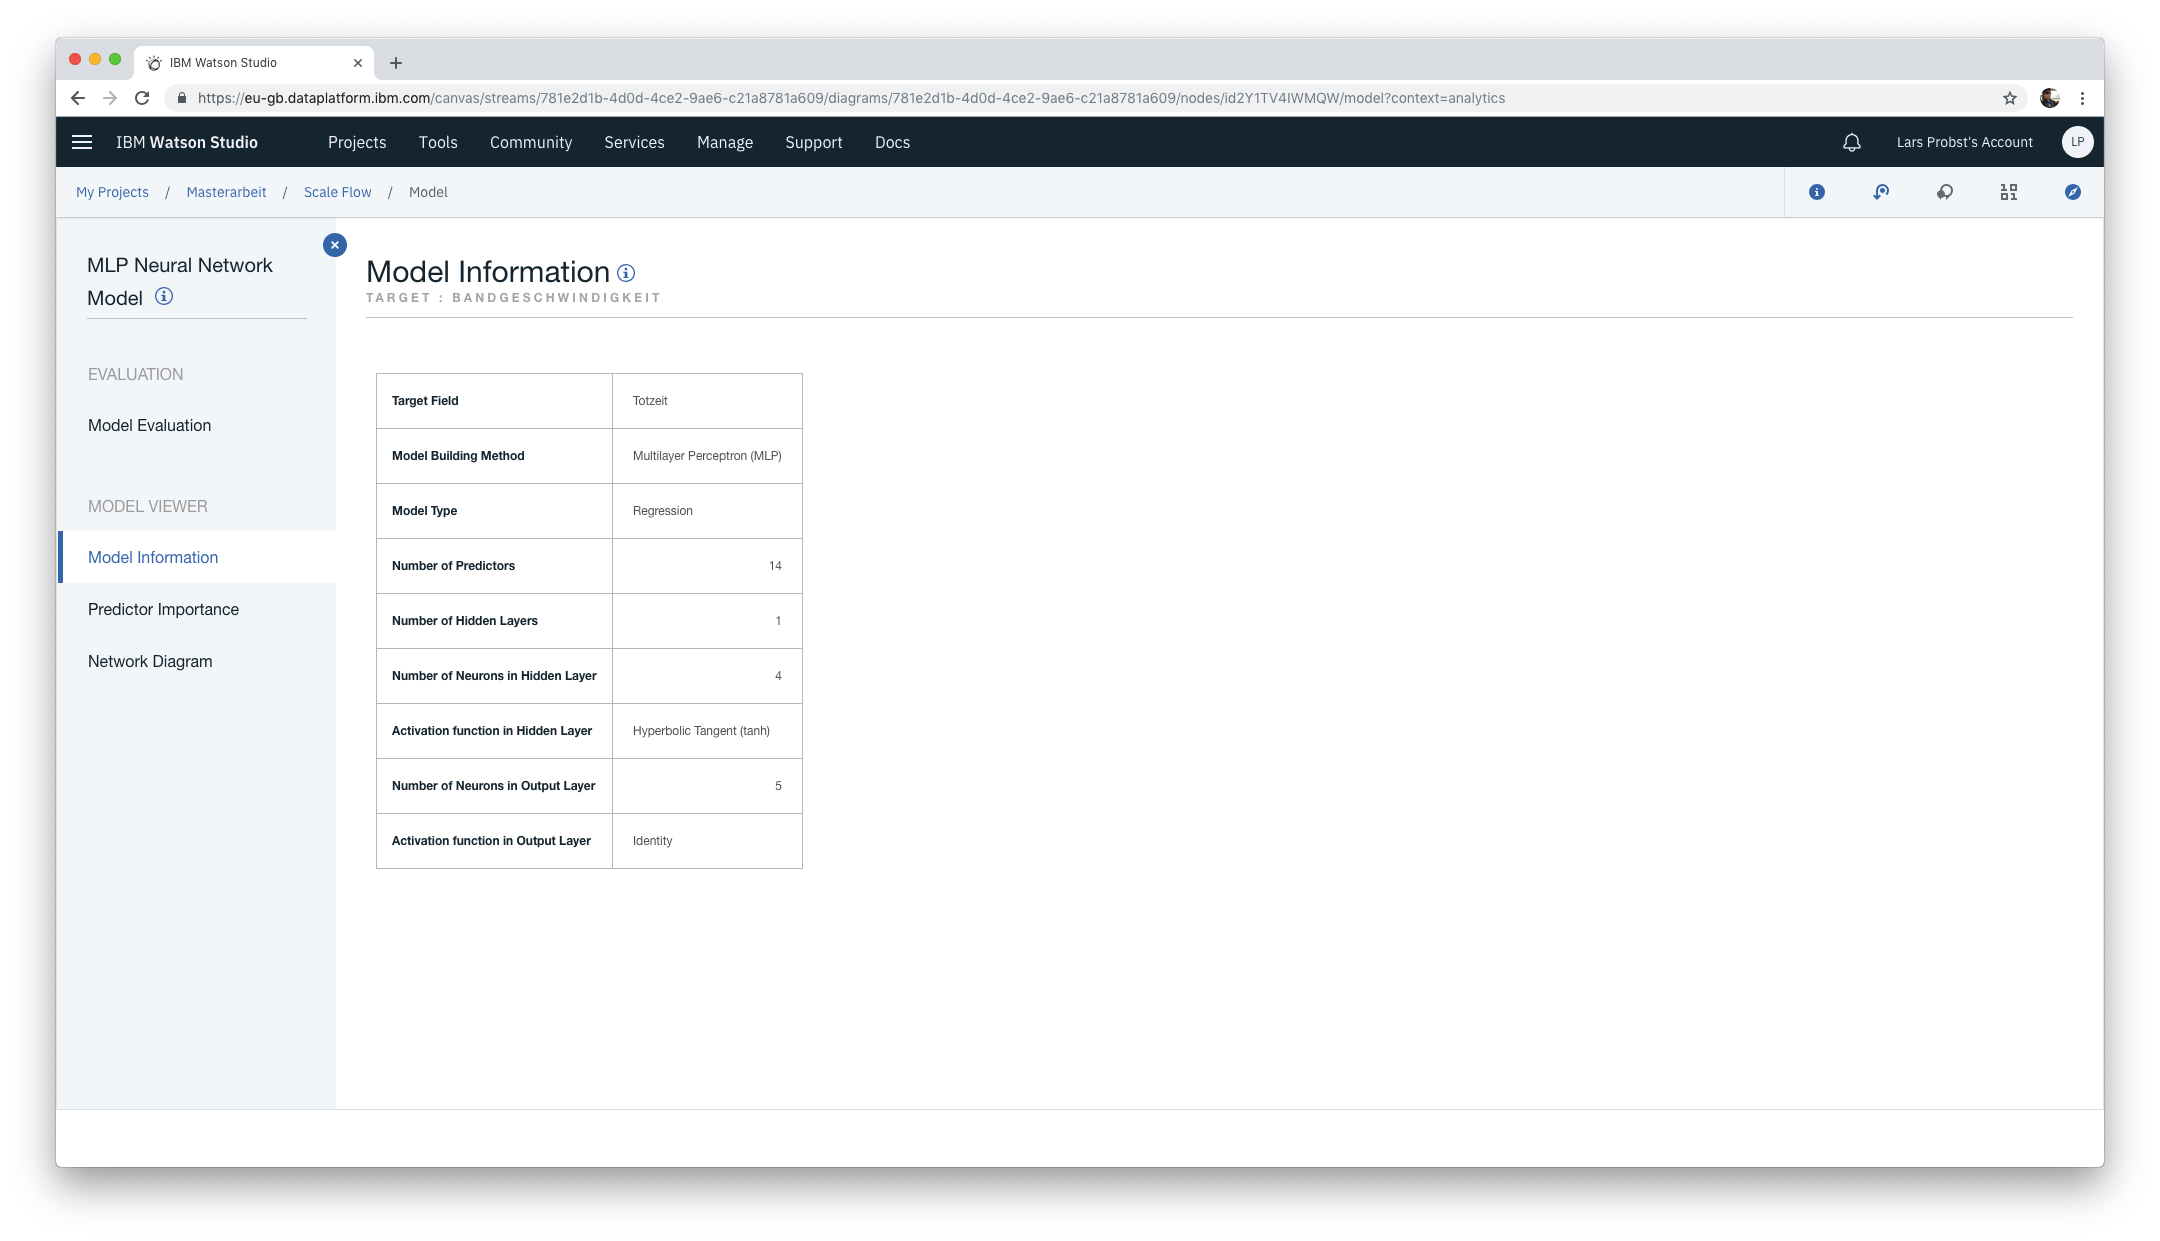
\includegraphics[width=\textwidth]{images/kapitel_3/model_information.png}
    \caption{Informtionen zum trinierten Model}
    \label{fig:umsetzung_model_information}
\end{figure}

Hier findet man Informationen darüber, wie das trainierte Model aufgebaut ist oder um welche Art Model es sich handelt.
Auch die Hiden Layers, die im neuronalen Netz eingerichtet sind, werden hier angegeben.

Weiter ist hier zu finden, mit wie vielen Inputparametern (englisch Number of Predictors) das Netz trainiert ist und wie
viele Ausgabewerte (englisch Number of Neurons in Output Layer) das Netz vorhersagen kann.

Im Menüpunkt \texttt{Predictor Importance} sind alle Input-Parameter aufgelistet. Ein Balken unterhalb jedes Parameters
gibt an, wie wichtig dieser für das neuronale Netz ist. In Abbildung~\ref{fig:umsetzung_model_predictor} auf
Seite~\pageref{fig:umsetzung_model_predictor} ist dies beispielhaft aufgezeigt.

\begin{figure}[h]
    \centering
    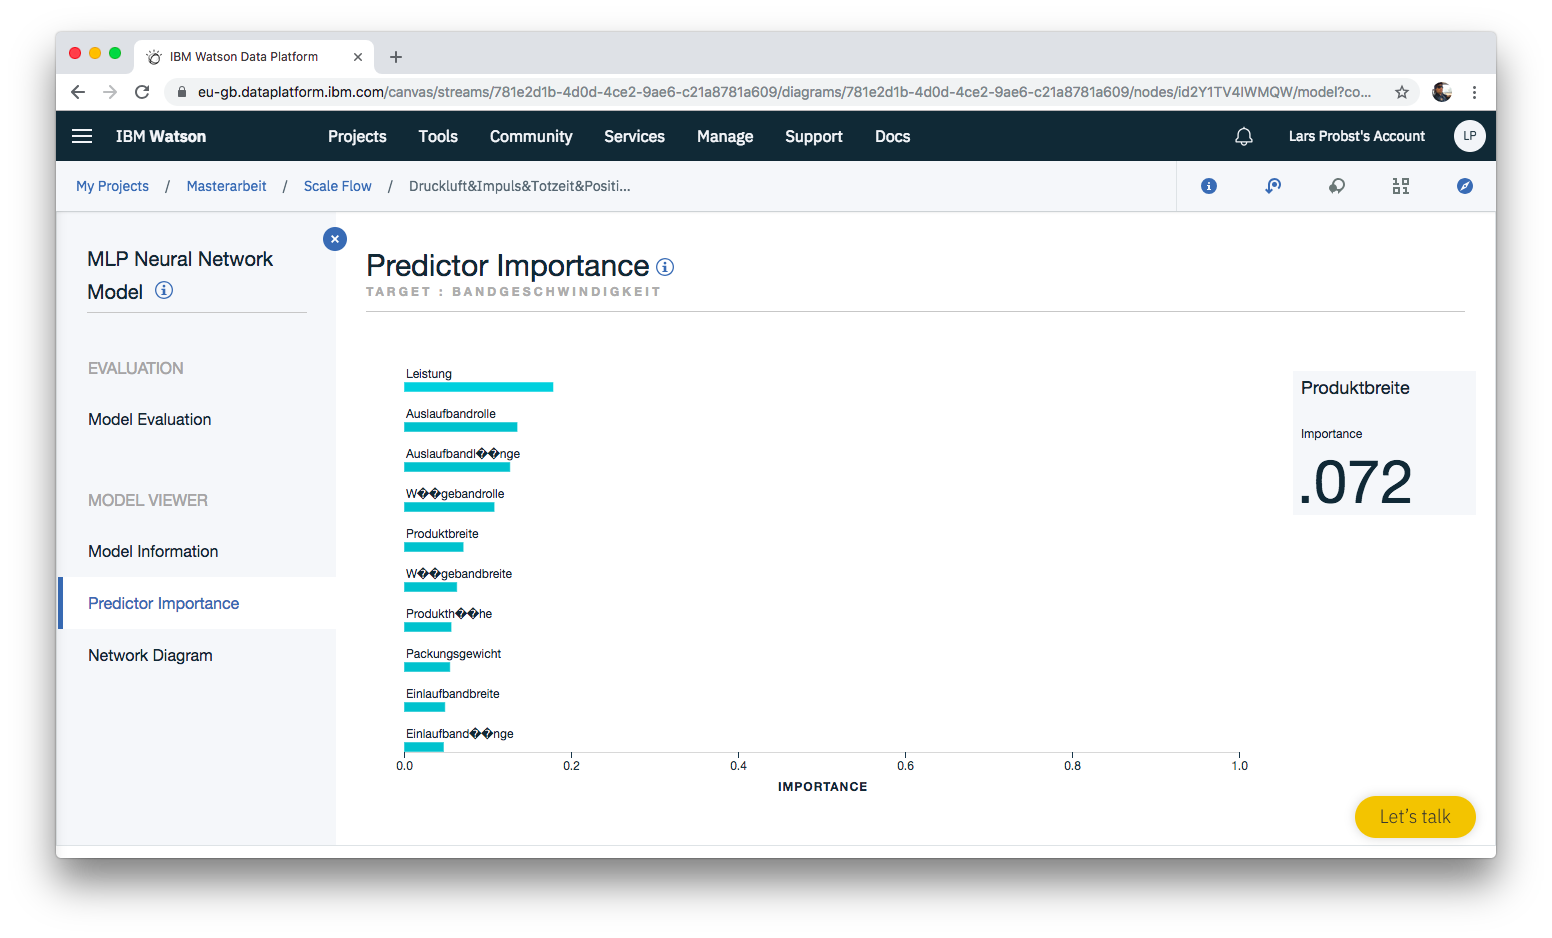
\includegraphics[width=\textwidth]{images/kapitel_3/model_predictor.png}
    \caption{Wichtigkeit der einzelnen Eingabeparameter}
    \label{fig:umsetzung_model_predictor}
\end{figure}

Beim Überfahren eines jeden Parameters wird der prozentuale Wert am rechten Rand dargestellt. Je wichtiger ein Parameter
ist, desto mehr Einfluss hat dieser auf die vorhergesagten Ausgabewerte.

Parameter mit der geringsten Gewichtung spielen für das Ergebnis keine große Rolle und könnten bei einer Optimierung des
neuronalen Netzes weggelassen werden.

Der letzte Menüpunkt, mit der Aufschrift \texttt{Network Diagram}, zeigt das neuronale Netz, wie es beim Traning aufgebaut
wurde. Dabei sind auf der linken Seite die Parameter zur Eingabe aufgelistet.

Auf der rechten Seite erscheinen die Ausgabeparameter. Dazwischen werden die \textit{Hidden Layers} dargestellt und wie
diese mit der Eingangs- und Ausgangsseite verbunden sind. Die Abbildung~\ref{fig:umsetzung_model_network_diagram}
auf~\pageref{fig:umsetzung_model_network_diagram} visualisiert das vorangegangene, trainierte Model.

\begin{figure}[h]
    \centering
    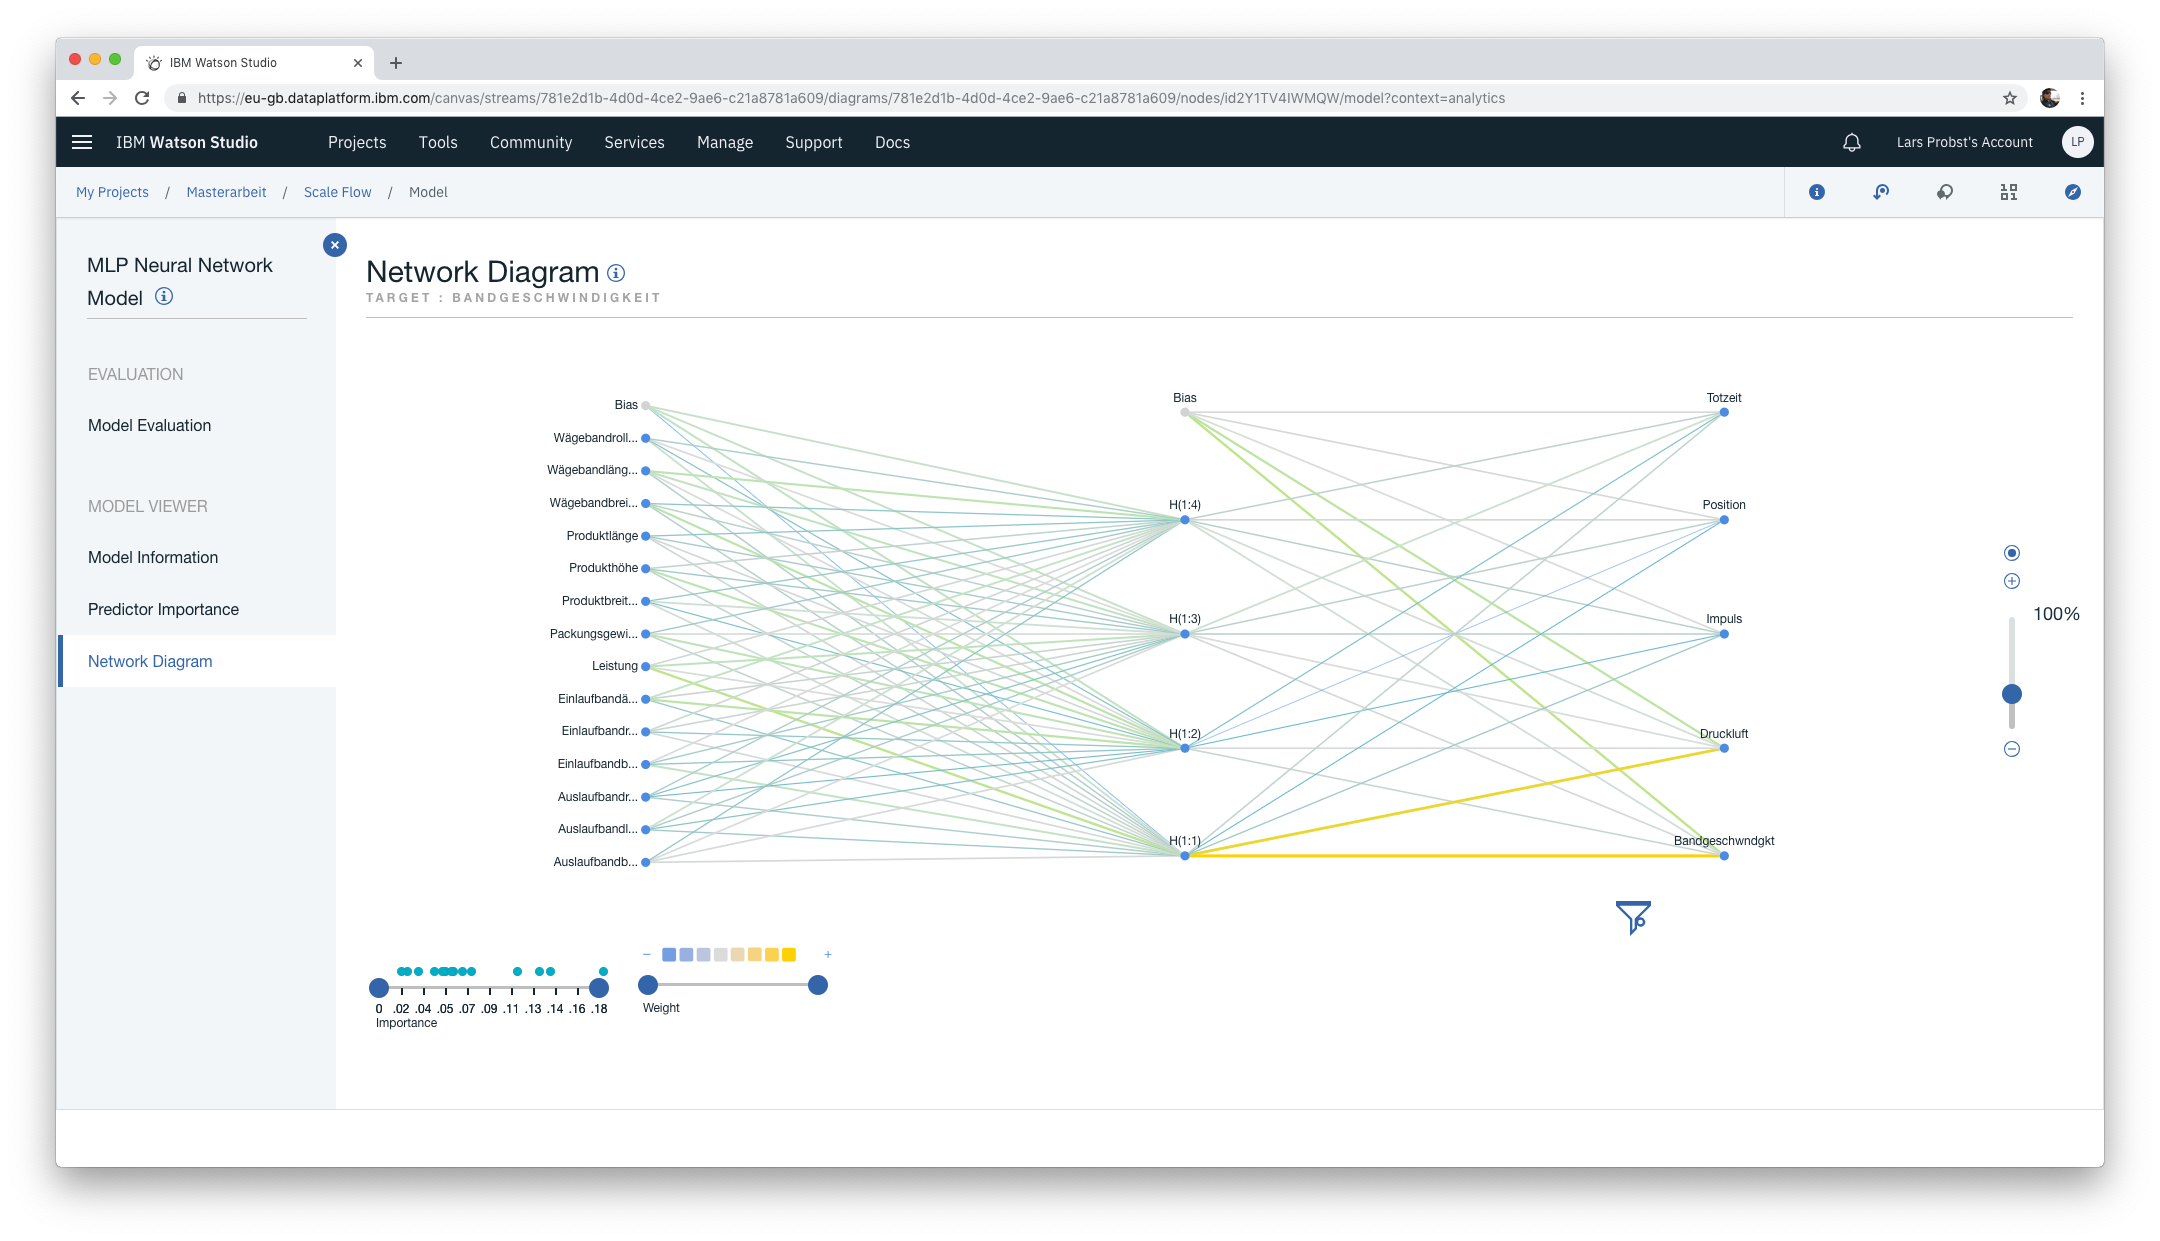
\includegraphics[width=\textwidth]{images/kapitel_3/model_network_diagram.png}
    \caption{Übersicht des trainierten Netzes}
    \label{fig:umsetzung_model_network_diagram}
\end{figure}

Die Ansicht kann man über den Slider am rechten Bildschirmrand vergrößern oder verkleinern. Über die Legende am unteren
Rand, kann man die einzelnen Verbindungen filtern.

So ist es zum Beispiel möglich, dass man sich alle Verbindungen mit hoher Priorität anzeigen lässt. Damit hat der
Entwickler eine Visualisierung, wie die wichtigsten Eingabeparameter für die entsprechenden Ausgaben sorgt.

Auch kann man sich so anzeigen lassen, wie einzelne Werte auf der Eingabeseite einen direkten Einfluss auf einen
Ausgabewert haben. Im Beispiel der Abbildung hat der Parameter \textit{Leistung} einen direkten und sehr großen
Einfluss auf den Ausgabewert \textit{Bandgeschwindigkeit}.

Bei weiterer Betrachtung ist diese Zusammenhang einläuchtend. Wenn mehr Produkte über die Wiegeeinheit laufen sollen (es
soll die Leistung erhöht werden), muss das Band mit höherer Geschwindigkeit (Bandgeschwindigkeit) laufen um die Produkte
zu transportieren.

Desweiteren hat die Leistung einen direkten Einfluss auf den Parameter \textit{Druckluft}. Dieser gibt indirekt die
Geschwindigkeit an, mit welcher der Pusher ausschlagen soll um ein Produkt vom Band zu hauen.

Auch dieser Zusammenhang ergibt Sinn, da eine höhere Bandgeschwindigkeit auch ein schnelleren Pusher voraussetzt, um ein
Produkt auch vom Band stoßen zu können. Das Timing ist an dieser Stelle von großer Bedeutung.

\subsubsection{Deployment erstellen}
Das in einem vorangegangenen Kapitel erstellte und trainierte Model kann man im Weiteren durch ein Deployment über eine
REST-Schnittstelle in einem Web-Dienst verfügbar machen.

Dazu ist es erforderlich, das Model in einen \texttt{Web service} zu installieren. Die spätere Wartung und Verwaltung
des Deployments wird dabei automatisch von der IBM Cloud übernommen.

Für die Erstellung des Web Services muss man im Watson Dashboard das zuvor erstellte Model auswählen. Das folgende
Fenster zeigt mehrere Informationen zu diesem an. Unter anderem ist sichtbar, welche Eingabe- und Ausgabeparameter für
das Model wichtig sind.

Der Reiter \texttt{Evaluation} zeigt vorangegangene Auswertungen des Models an. Über den Menüpunkt \texttt{Lineage}
werden Verknüpfungen und Abstammungen des Models angezeigt.

Für das Deployment ist der Reiter \texttt{Deployments} wichtig. Dieser verwaltet alle Deployments des einen Moduls. Das
Löschen von älteren Deployments oder das Erstellen von Neuen ist hier möglich. Die Schaltfläche \texttt{Add Deployment}
öffnet eine Konfigurationsseite zum Erstellen eines neuen Deployments.

Ein Model kann über mehrere Deployments verfügbar gemacht werden. So ist es möglich, die Last eines Web-Services zu
reduzieren bzw. auf mehrere zu verteilen. Um die Last zu verteilen bedarf es eines Load-Balancers.

Als Type für das Deployment muss man \textit{Web Service} auswählen. Der Name des Deployments ist das einzige Pflichtfeld
und muss befüllt sein. Anschließend kann man das Deployment über \texttt{Save} speichern und starten. Dieser Vorgang kann
wenige Minuten dauern.

Direkt nachdem das Deployment fertiggestellt ist, wird in der Spalte \textit{Status} der Wert \texttt{DEPLOY\_SUCCESS}
angezeigt. Die Informationsseite des Deployments kann man über einen Klick auf den Namen öffnen.

Das Deployment ist somit erfolgreich erstellt und kann im Weiteren getestet und genutzt werden.

\subsubsection{Deployment testen}
Ein online Test des eingerichteten Deployments ist über das Watson Studio Dashboard möglich. Dies hat den Vorteil, dass
man das Deployment direkt testen und bei Fehlveralten neu trainiert kann. Auch benötigt man keine externe Software um
das Model zu testen.

Auf der Deploymentseite des gespeicherten Models genügt ein Klick auf den Namen um die Deploymentinformationen anzuzeigen.
Hier steht neben diversen Informationen auch der Menüpunkt \texttt{Test} zur Verfügung. Mit diesem öffnet sich eine
zweispaltige Ansicht.

In der linken Spalte befinden sich die Eingabefelder für das trainierte Model (die Inputs). Nachdem man alle Felder mit
Testwerten gefüllt hat, kann man über die Schaltfläche \texttt{Predict} eine Vorhersage starten.

Nach wenigen Sekunden erscheint auf der rechten Seite ein großes JSON-Objekt, welches den Rückgabewert des Web Services
enthält. Das erste Array, \textit{fields}, listet alle an den Web-Service gesendeten Felder auf (die Inputs).

Das zweite Array, \textit{values}, listet alle an den Web-Service gesendeten, wie auch die vorhergesagten Werte (die
Inputs und die Targets) auf. Die letzten fünf Werte des Arrays entsprechen den Vorhersagen des trainierten Models (also
die Targets). Sie entsprechen den definierten Targets.

In Abbildung~\ref{fig:umsetzung_deployment_test} auf Seite~\pageref{fig:umsetzung_deployment_test} ist ein Beispiel für
den online Aufruf des trainierten Models sichtbar.

Sollte das Array \textit{values} kleiner sein, als das Array \textit{fields}, war das trainieren des Models nicht
erfolgreich und muss wiederholt werden. Das Model kennt damit keine Targets die es vorhersagen könnte.

Unter dem Menüpunkt \texttt{Implementation} sind wichtige Informationen und erforderliche Schritte aufgezeigt, damit
man die erstellte Schnittstelle in ein eigene Programm integriert kann. Dabei wird auf verschiedene Programmiersprachen
und Architekturen eingegangenund.

\begin{figure}[h]
    \centering
    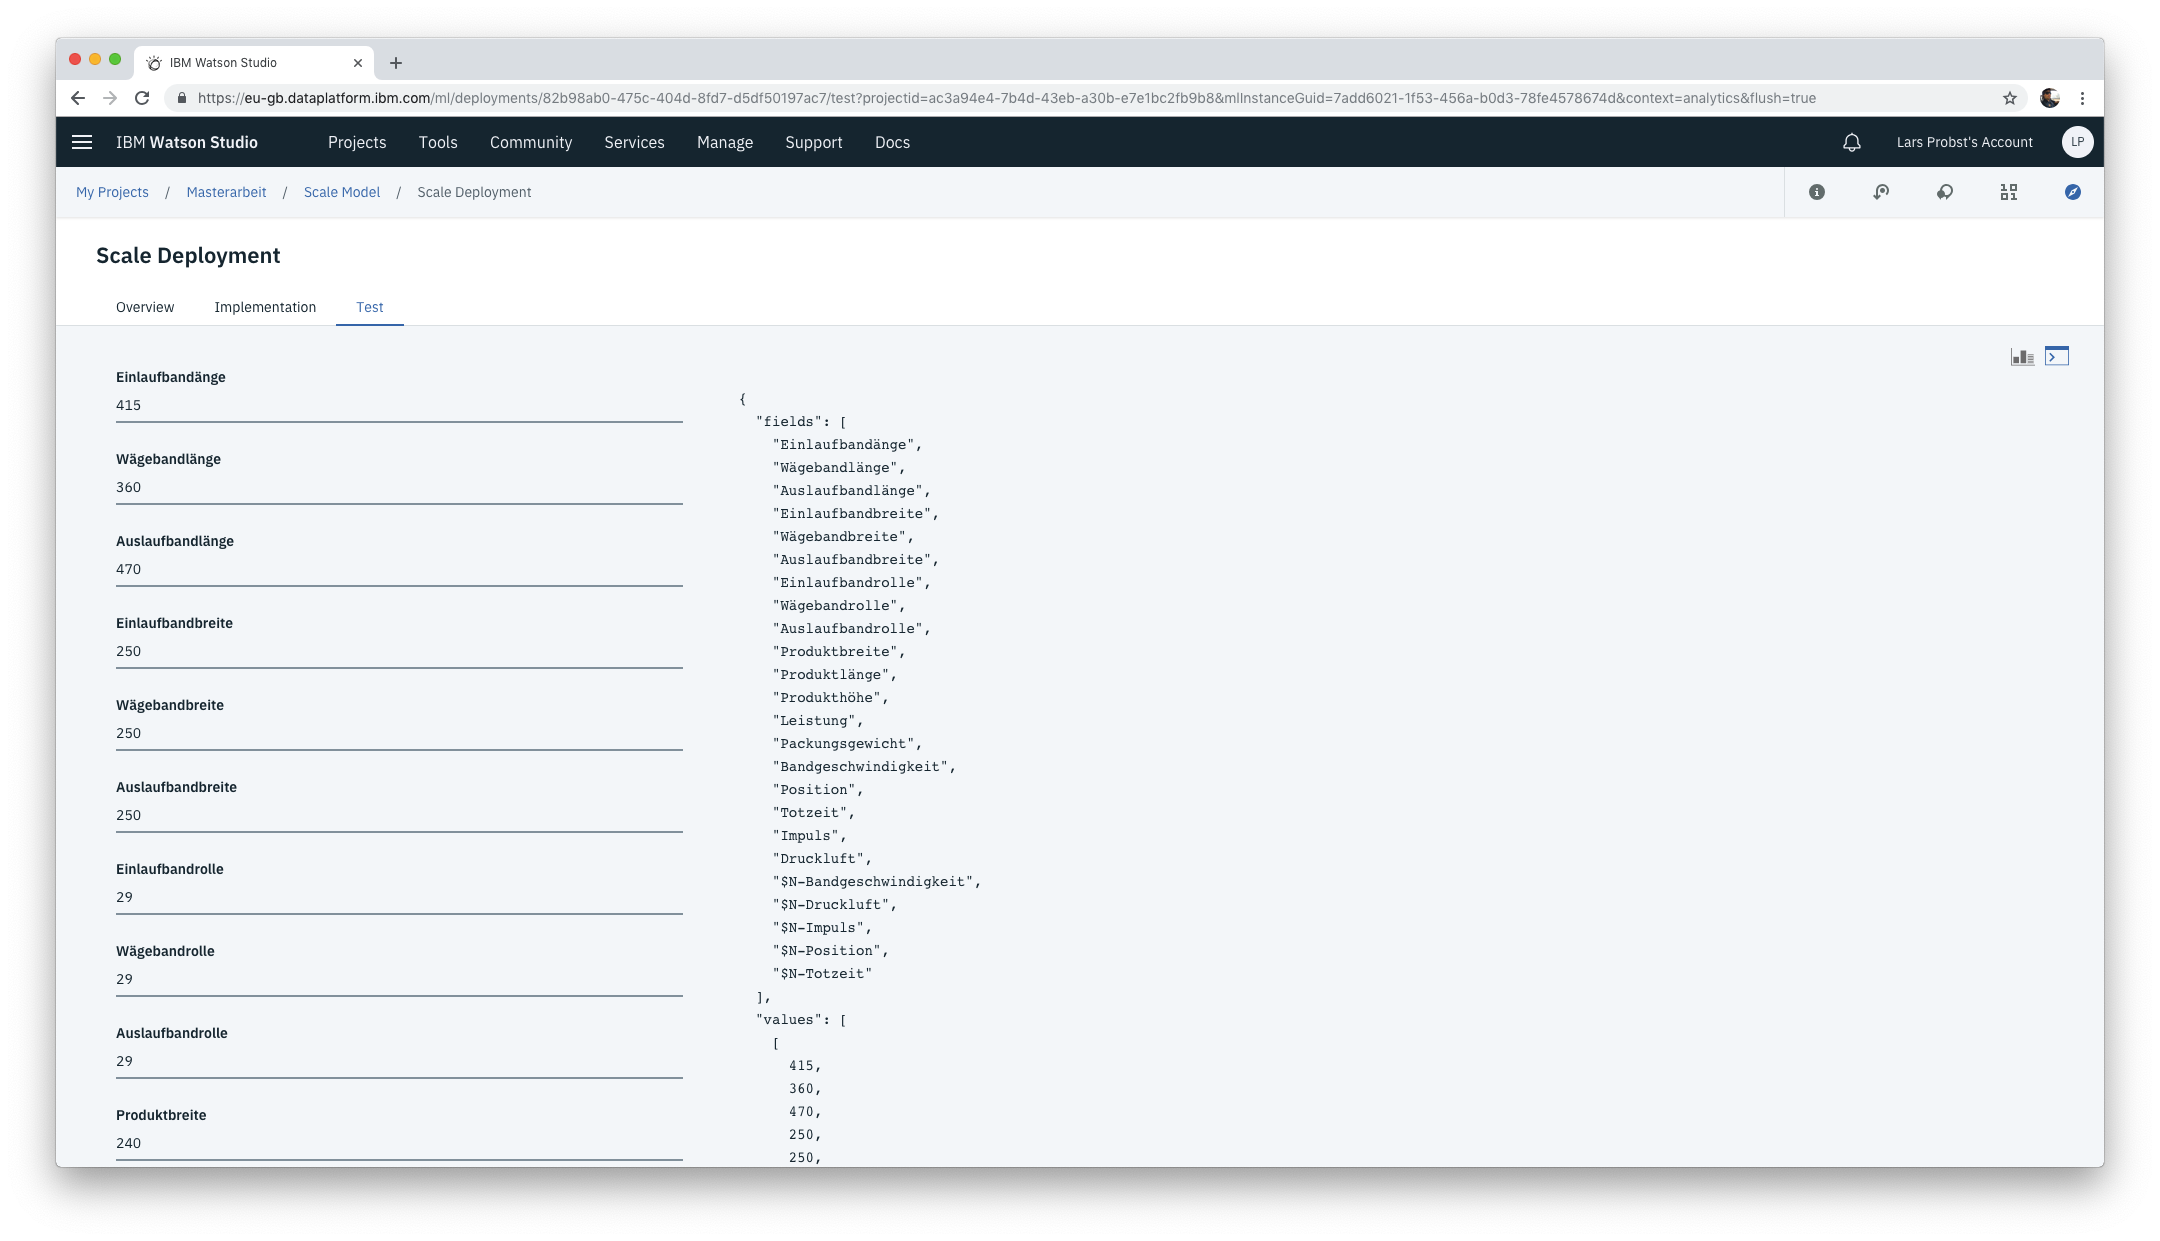
\includegraphics[width=\textwidth]{images/kapitel_3/deployment_test.png}
    \caption{Online Test des trainierten Models}
    \label{fig:umsetzung_deployment_test}
\end{figure}

\subsubsection{Aufruf mit Postman}
\label{subsec:Aufruf mit Postman}
Im Weiteren soll das erstellte Model, welches im vorherigen Kapitel als Deployment in einen Web-Service zur Verfügung
gestellt wurde, mit Postman\footnote{https://www.getpostman.com} getestet werden.

So ist sichergestellt, dass man das Model auch von extern, nicht nur über das Watson Studio Dashboard, aufrufen kann.
Dies ist für die spätere Entwicklung des Frontends und die Einrichtung des API Connect Services wichtig. Außerdem ist
so eine Überprüfung der Übergabeparameter, sowie der Rückgabewerte an die Schnittstelle möglich.

Jeder Request an den Web-Service des trainierte Models benötigt einen \textit{Authentication Token} (kurz Auth-Token).
Dieser Token stellt sicher, dass es sich um einen gültigen Aufruf handelt.

Über die REST-Schnittstelle des Watson Studios wird ein neuer Token generriert. Dabei handelt es sich um eine andere
Schnittstelle als beim selbst erstellten Web-Service. Der Token ist immer nur für maximal vier Stunden gültig.

Um einen Auth-Token zu erstellen, muss man den Watson Studio Benutzername und das zugehörige Passwort an die Schnittstelle
übergeben. Ein Beispielaufruf ist in Listing~\ref{ls:umsetzung_apitoken} auf Seite~\pageref{ls:umsetzung_apitoken}
zu sehen. Der Token ist dabei in einem JSON-Objekt im Rückgabewert enthalten.

\begin{lstlisting}[language=bash, caption=Abruf des Auth-Tokens, label=ls:umsetzung_apitoken]
$ curl --basic --user USERNAME:PASSWORD https://eu-gb.ml.cloud.ibm.com/v3/identity/token
\end{lstlisting}

Die Parameter \texttt{USERNAME} und \texttt{PASSWORD} muss man durch die entsprechenden Werte ersetzen. Im folgenden
mehr dazu.

In Postman kann man diesen Aufruf über die Eingabe der URL und dem HTTP-Type \texttt{GET} machen. Im Reiter
\textit{Authentication} ist der Type \textit{Basic-Auth} auszuwählen.

Im rechten Bereich sollten dann die beiden Eingabefelder für Benutzername und Passwort erscheinen. Der Nutzer muss die
geforderten Daten eingeben und kann dann den Request mit der Schaltfläche \texttt{Send} starten.

Den Benutzernamen und das zugehörige Passwort findet man in der Übersichtsseite des Machine Learning Services. Diese
Seite erreicht man über einen Klick auf den Machine Learning Service auf dem IBM Cloud Dashboard. Auf der linken Seite
kann man sich über den Menüpunkt \texttt{Serviceberechtigungsnachweise} und dann über die Schaltfläche
\texttt{Berechtigungsnachweise anzeigen} die Daten anzeigen lassen.

Nach wenigen Sekunden erscheint im Bereich \textit{Body} der Token in einem JSON-Objekt. Ähnlich dem Aufruf mit
\textit{curl}.

Um nun das eigentliche Deployment aufzurufen, muss man einen neuen Postman-Tab öffnen. Die URL für den Endpunkt ist im
Deployment des Models zu finden und heißt \texttt{Scoring End-point}.

Nachdem die URL des Postman-Requests definiert ist, kann man als HTTP-Type \texttt{POST} auswählen. Im Bereich
\texttt{Authentication} wird der Typ auf \texttt{Baerer} abgeändert und dies ermöglicht die Eingabe des Tokens. Dieser
Token entspricht dem Rückgabewert des vorangegangenen Postman-Requests.

Die Auswahl des HTTP-Types \textit{POST} ermöglicht die Definition des Bereichs \texttt{Body} für den Request. Dabei
handelt es sich um Parameter, welche an die Schnittstelle geschickt werden.

Als Datentyp muss man \textit{raw} und als Type \textit{JSON (application/json)} auswählen. Im
Anhang~\ref{sec:postmanTestparameter} auf Seite~\pageref{sec:postmanTestparameter} sind Testparameter zu finden, welche als
Eingabe genutzt werden können.

Der Nutzer kann abschließend den Request über den Button \texttt{Send} an den Web-Service abschicken. Nach wenigen
Sekunden zeigt Postman den erhaltenen Response des neuronalen Netzes an. Hier sollten auch die Vorhersagen enthalten sein.

In der Abbildung~\ref{fig:umsetzung_deployment_postman} auf Seite~\pageref{fig:umsetzung_deployment_postman} ist ein
Beispielrequest aus Postman auf das Deployment zu sehen. Im linken Bereich sieht man das gesendete JSON-Objekt, mit den
Eingabevariablen (Inputs). Dabei hat das JSON-Objekt die beiden geforderten Items \textit{fields} und \textit{values}.

\begin{figure}[h]
    \centering
    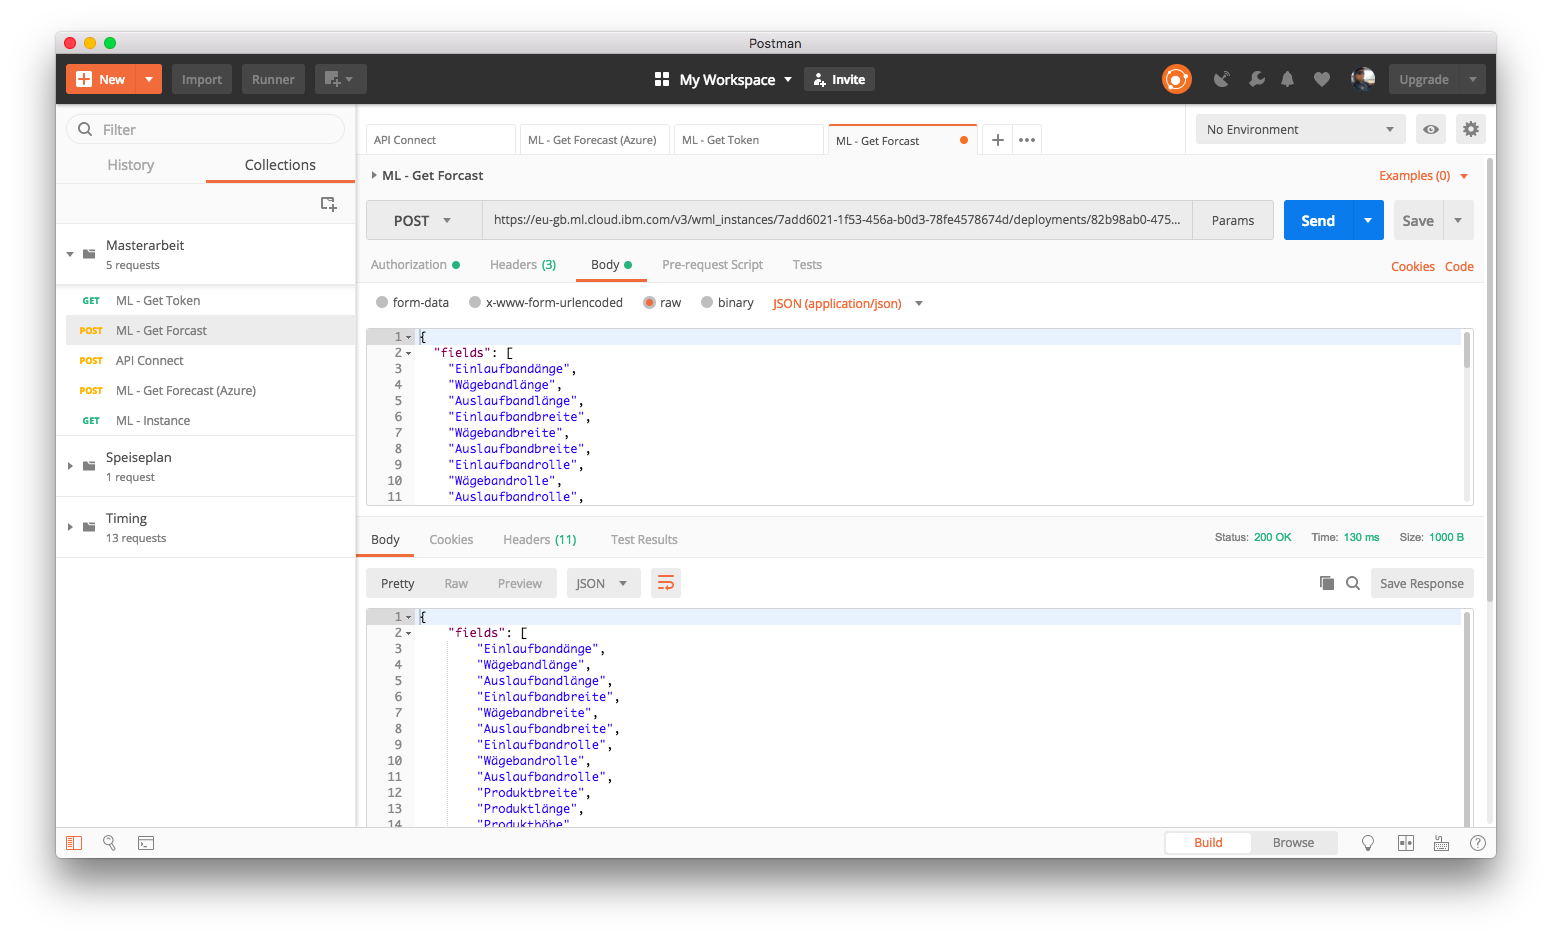
\includegraphics[width=\textwidth]{images/kapitel_3/deployment_postman.png}
    \caption{Beispielrequest von Postman}
    \label{fig:umsetzung_deployment_postman}
\end{figure}

Die Rechte Seite zeigt die Antwort des Web-Service. Dabei werden zu Anfang des JSON-Objektes die Parameter wiederholt,
die an das Interface gesendet wurden. Am Ende sind die vorhergesagten Parameter durch das trainierte Model zu sehen.

Im Eingabe-Parameter \textit{values} muss man ebenfalls die Output-Parameter definieren. Da die Werte keine Rolle
spielen, kann man diese mit den Werten \textit{null} initialisieren. Damit werden sie vom System nicht weiter verwendet.

Auf der Übersichtsseite des REST-Interfaces des
Deployments\footnote{https://watson\-ml\-api.mybluemix.net/?cm\_mc\_uid=61889453441915363064337}, sind noch weitere
Endpunkte und die dafür benötigten Parameter sowie die Rückgabewerte ersichtlich.

\subsection{TensorFlow.js}
Das neuronale Netz ist nun erfolgreich in einem Deployment online zur Verfügung gestellt. Außerdem ist die Funktion
über einen Aufruf mittels Postman überprüft worden. Im Weiteren wird das trainierte Model in eine TensorFlow.js
Applikation eingebaut.

Dies hat nun mehrere Vorteile. Zum einen kann man das trainierte Model unabhängig von einer Cloud-Lösung nutzen. Die
TensorFlow.js Applikation kann zum Beispiel in einen Cloud Foundry-Container geladen werden und ist somit völlig unabhängig
von der Plattform auf der die Applikation läuft. Auch kann sie modular und schnell in beliebigen Regionen instanziiert
werden.

Ein weiterer Vorteil ist die Unabhängigkeit welche damit erreichbar wird. Die Applikation kann selbst verwaltet,
instanziiert oder auch aktualisiert werden.

Natürlich ist es ebenfalls möglich die TensorFlow.js Applikation direkt in die eigene Hauptapplikation zu integrieren
ohne sie als Microservice nutzen zu müssen.

\subsubsection{Model exportieren}
Damit das Model in die TensorFlow.js Applikation eingebunden werden kann, muss es aus dem Watson Studio exportiert werden.
Dies erfolgt über den Modeler Flow.

Da der Entwickler das Model in Kapitel~\ref{subsub:modeler_flow} auf Seite\pageref{subsub:modeler_flow} komplet
eingerichtet und trainiert hat, steht es im Modeler Flow als gelbes Modul bereit.

Über einen Rechtsklick auf das trainierte Model und dem Menüpunkt \texttt{Download Model} kann man das Model auf den
Entwicklungsrechner herunterladen. Bei der Datei handelt es sich um eine pb-Datei. Diese Datei beinhaltet alle wichtigen
Informationen über das gebaute neuronale Netz.

Auf der Seite des
FreeCodeCamps\footnote{https://medium.freecodecamp.org/how-to-deploy-tensorflow-models-to-production-using-tf-serving-4b4b78d41700}
ist eine Beschreibung und der interne Aufbau der gespeicherten Datei ersichtlich. Auch wird dort erklärt, wie die Datei
in andere Anwendungen importiert werden kann.

Im Weiteren kann mit der Entwicklung des Wrappers für das heruntergeladene neuronale Netz begonnen werden. Dafür wird
der Inhalt der Datei in einer TensorFlow.js Applikation importiert und ausgewertet.

\subsubsection{Wrapper entwickeln}
Da das trainierte Model nun offline zur Verfügung steht, kann es im Weiteren mit TensorFlow.js in einem Node.js-Wrapper
genutzt werden.

Die Idee des Wrappers ist es, ein Web-Service zur Verfügung zu stellen, der auf dem Port 80 eine REST-Schnittstelle
beherbergt. Dort findet sich mindestens ein REST-Endpunkt, welcher die Input-Parametern für das trainiert,
neuronale Netz annehmen kann.

Die übergebenen Werte werden anschließend von einer Routine extrahiert und über die TensorFlow.js Bibliothek an das
heruntergeladene neuronale Netz übergeben.

Anschließend übermittelt der Web-Service die durch das neuronale Netz vorhergesagten Parameter zurück an die Applikation,
welche die Anfrage gestellt hat.

Für die Umsetzung des Wrappers sind also zwei Bestandteile elementar. Einerseits muss die Anwendung eine TensorFlow.js
Umgebung schaffen, indem man das heruntergeladene und trainierte Netz einbinden kann. Andererseits muss es eine
REST-Schnittstelle bieten, damit man es von über den API Connect Service ansprechen kann.

Bei der Entwicklung beginnt man am Besten beim REST-Endpunkt, da dieser die Struktur der Anwendung vorgibt. Für die
Implementierung der Endpunkte sind die Libraries \textit{express}\footnote{https://expressjs.com/de} und
\textit{body-parser}\footnote{https://github.com/expressjs/body-parser} sehr hilfreich.

Die \textit{express}-Bibliothek unterstützt bei der Entwicklung eines Web-Servers, welchen man anschließend über den
Port 80 ansprechen kann. Der \textit{body-parser} kümmert sich um das Auslesen der übergebenen Parameter an die
Schnittstelle oder das Bündeln der Rückgabewerte - also um den Umgang mit JSON-Objekten.

Da Node.js und damit der Paketmanager npm schon installiert ist, kann der Entwickler mit \textit{npm init} ein neues 
Projekt starten. Wenn man diesen Befehl in einem noch leeren Ordner ausführt, erscheint eine neue Datei mit dem Namen
\textit{package.json}. In dieser Datei werden unter anderem alle benötigten Abhängigkeiten des Projektes aufgelistet 
um sie später einfach und komfortabel zu installieren.

Hinter den einzelnen Bibliotheken kann man direkt die Version definieren, welche man nutzen möchte. Im Listing ist ein
\textbf{\^}-Symbol vorangestellt. Dies bedeutet, dass die Version, welche heruntergeladen werden soll, zu der angegebenen
Version kompatibel sein muss. Das bedeutet, dass durchaus eine andere Version heruntergeladen werden kann, falls eine
neuere existiert. Allerdings bietet sie mindestens genau die selben Funktionen wie die geforderte.

Auch werden in der Datei der Name, eine Beschreibung und die Version des Projektes angegeben. Außerdem kann man Skripte
definieren, welche man durch kurze Befehle in ein Terminal ausführen kann. Dazu später mehr.

In Listing~\ref{ls:umsetzung_package} auf Seite~\pageref{ls:umsetzung_package} ist die vollständige package.json-Datei
ersichtlich, welche die beiden Bibliotheken als Abhängigkeit entählt und ein paar wenige Parameter wie Name, Beschreibung, 
Version und verwendete Lizenz angibt. 

Auch ist ein script mit dem Namen \textit{start} angegeben. Dies kann später mit dem Befehl \textit{npm start} starten.
Die definition für den Startbefehl kümmert sich anschließend darum, dass intern der Befehl \textit{node server.js}
ausgeführt wird. Diese Datei wird im Weiteren erstellt.

\begin{lstlisting}[language=json, caption=Die komplette package.json, label=ls:umsetzung_package]
{
    "name": "tensorflow_wrapper",
    "version": "1.0.0",
    "description": "A rest-wrapper for a tensorflow net.",
    "main": "server.js",
    "scripts": {
        "start": "node server.js"
    },
    "author": "Lars Helmuth Probst <lars@famprobst.de>",
    "license": "ISC",
    "dependencies": {
        "body-parser": "^1.18.3",
        "express": "^4.16.4",
        "tensorflow/tfjs": "",
        "ensorflow/tfjs-node": "",
        "tensorflow/tfjs": "",
        "tensorflow/tfjs-node-gpu": ""
    }
}
\end{lstlisting}

Im selben Ordner wie die angelegte package.json kann man nun mittels des Befehls \textit{npm install} alle Abhängigkeiten 
in das Projekt installieren. 

Auch wenn eine selbst benötigte Bibliothek, wie zum Beispiel die express-Library, weitere Abhängigkeiten benötigt, werden 
diese automatisch mitinstalliert. So ist sichergestellt, dass alle geforderten Bibliotheken einwandfrei funktionieren.

Die Ausführung des Befehls hat zur Folge, dass ein neuer Ordner mit dem Namen \textit{node\_modules} erstellt wird. In diesem 
finden sich nun alle geforderten Bibliotheken und deren Abhängigkeiten an einem zentralen Ort und sind zur Verwendung bereit.

Als nächstes kann man mit der Entwicklung des REST-Endpunktes beginnen. Dafür wird eine initiale Datei benötigt, in der der
Express-Server sowie alle REST-Endpunkte definiert sind. 

Diese Datei trägt den Namen \textit{server.js} und ist in Listing~\ref{ls:umsetzung_serverjs} auf 
Seite~\pageref{ls:umsetzung_serverjs} zu sehen. In den ersten vier Zeilen der Datei werden die benötigten Bibliotheken in das 
Programm geladen um sie für andere Routinen verfügbar zu machen. Der Express-Server und der Body-Parser sind somit 
einsatzbereit.

In der sechsten Zeile wird in der Variable \textit{app} die Instanz des Express-Servers gespeichert. Somit kann man diesen über
die Variable konfigurieren.

\begin{lstlisting}[language=JavaScript, caption=Die komplette server.js, label=ls:umsetzung_serverjs]
const express = require('express');
const bodyParser = require('body-parser');
const tf = require('@tensorflow/tfjs')
require('@tensorflow/tfjs-node')

const app = express();

app.use(bodyParser.urlencoded({ extended: true }));

app.post('/predict-tensorflow', (req, res) => {
    // TODO TensorFlow.js
    res.send(req.body)
});

app.listen(80, () => {
    console.log('server listening on port 80.');
});
\end{lstlisting}

Die achte Zeile sorgt dafür, dass man \textit{URL-Encoded}-Daten an den REST-Endpunkt schicken kann und man diese dann
verwenden kann. Andernfalls müssten alle Anfragen gesondert geparst werden.

Mit den Zeile zehn bis 13 wird ein Endpunkt für den Express-Server definiert, welcher in einem weiteren Schritt mit der
TensorFlow.js Logik gefüllt wird. Der Endpunkt hat den Namen \textit{predict-tensorflow} und als HTTP-Typ ist \textit{POST}
angegeben. Damit können Daten an den Endpunkt geschickt werden.

Mit der Zeile zwölf werden alle Daten und Informationen, welche an den Endpunkt geschickt werden, auch wieder zurückgegeben. Dies
dient als ein Test für das richtige Versenden und die richtige Funktion des Endpunktes.

Die letzten drei Zeilen lassen den Express-Server auf Port 80 starten und geben Auskunft darüber, dass der Start des Servers
erfolgreich war.

Im Weitern kann nun die Zeile elf so erweitert werden, dass die mitgeschickten Daten auch an das heruntergeladene neuronale
Netz übergeben werden können. Dies wird durch die Hilfe von TensorFlow.js ermöglicht.

In Listing~\ref{ls:umsetzung_tensorflow} auf Seite~\pageref{ls:umsetzung_tensorflow} sind alle Änderungen für den Einbau des
TensorFlow.js-Wrappers aufgeführt.

\begin{lstlisting}[language=JavaScript, caption=Der TensorFlow.js Programmteil, label=ls:umsetzung_tensorflow]
const mn = new mobilenet.MobileNet(1, 1);
mn.path = "./neural_net.json"
await mn.load()

const predictions = await mn_model.classify(req.body);
res.send(predictions);
\end{lstlisting}

Die Zeilen eins bis drei kümmern sich um das Laden des trainierten Netz von der Festplatte. In der sechsten Zeile werden
die übergebenen Daten des REST-Endpunktes an die TensorFlow.js-Instanz weitergegeben um eine Vorhersage zu erhalten. Über 
die letzte Zeile werden die vorhergesagten Parameter wieder zurückgegeben.

Diese Zeilen muss man nun lediglich in die Datei \textit{server.js} in die Zeile elf kopieren, damit die REST-Schnittstelle
vollkommen ist.

Die entwickelte Applikation soll im Weiteren über eine Domain aus dem Internet aufrufbar sein. Eine Installation in einen
Cloud Foundry-Container, welcher in der IBM Cloud läuft, ist dafür notwendig. Im folgenden Kapitel werden die dafür
nötigen Schritte erläutert.

\subsubsection{Toolchain einrichten}
Die fertig entwickelte Node.js Applikation wird im nächsten Schritt in einen Cloud Foundry-Container installiert. Dies
ermöglicht den Aufruf der Applikation über eine Domain, welche automatisch von der IBM Cloud vergeben wird.

Damit man den geschriebenen Quellcode nicht nach jeder Änderung manuell mittels \texttt{cf push} in einen Cloud
Foundry-Container laden muss, wird hierfür eine Toolchain aus der IBM Cloud genutzt.

Die Nutzung der Toolchain erfordert ein eingerichtetes Git-Repository. Nach jedem \texttt{commit}, welchen man in dieses
Repository schreibt, aktiviert sich die Toolchain selbstständig und lädt den entsprechenden Commit herunter.

Anschließend werden, je nach gewählter und eingerichteter Konfiguration, verschiedene Schritte (Phasen) in der Toolchain
durchlaufen, um die Applikation in einen Cloud Foundry-Container zu installieren.

Dabei ist es möglich die einzelnen Schritte, welche bei einem Deployment durchlaufen werden, selbst zu definieren, oder
eine vorkonfigurierte Toolchain zu nutzen. Es ist allerdings möglich die vorkonfigurierte Toolchain im Nachgang zu
individualisieren. Sie dient lediglich einem schnelleren Start.

Für die Konfiguration der Toolchain muss man die instanziierte Node.js Runtime, in welcher die entwickelte Applikation
laufen soll, in dem IBM Cloud Dashboard auswählen.

Auf der dann folgenden Seite im Tab \texttt{Übersicht} (linke Seite) erscheinen fünf Kacheln mit unterschiedlichen
Informationen. Für die Toolchain ist die Karte mit der Aufschrift \texttt{Continous Delivery} entscheidend. Dort gibt es
einen Button mit der Aufschrift \texttt{Aktivieren}.

Ein Klick auf diesen öffnet die Übersicht und eine visuelle Vorschau der Standardkonfiguration der Toolchain. Nun muss
man einen Name eintragen und die Region auswählen, in der die Toolchain installiert wird. Da die Standardkonfiguration
vorerst völlig ausreichend ist, kann diese direkt übernommen werden. Dafür genügt ein Klick auf \texttt{Erstellen}.

Nach einem kurzen Ladevorgang ist die Toolchain eingerichtet und vorkonfiguriert. Es erscheinen nun vier Karten für
unterschiedliche Bereiche, in denen die IBM Cloud dem Entwicklungszyklus helfen kann.

Im Bereich \texttt{Nachdenken} wird ein Issue-Tracker konfiguriert, in dem zum Beispiel Bugs (Softwarefehler), welche
in der Software entdeckt werden, eingetragen, verwaltet und diskutiert werden können.

In \texttt{Codieren} stehen gleich zwei Kacheln zur Verfügung. Einerseits das konfigurierte Git-Repository, bei dem es
sich um ein auf IBM-Servern gehostetes GitLab handelt. Andererseits findet sich dort eine Web-IDE auf Basis von Eclipse
Orion, mit der der Quellcode der Anwendung online editiert werden kann.

In der letzten Kategorie, \texttt{Bereitstellen}, findet sich die Pipeline, welche im nächsten Schritt näher erläutert
und eingerichtet wird. Mit einem Klick auf die Kachel mit der Aufschrift \texttt{Delivery Pipeline} wechselt man in die
Konfiguration.

Nach dem Laden der Seite erscheinen zwei sogenannte \textit{Phasen} (engl. Stages). Jeder Schritt in der Delivery Pipeline
wird durch eine Phase symbolisiert. In einer Phase können zum Beispiel der Quellcode aus dem Git-Repository geladen, oder
die geschriebenen Tests durchgeführt werden.

Die Standardkonfiguration sieht in der \textit{Build Stage} das Herunterladen des Quellcodes aus dem Git-Repository vor
und in der \textit{Deploy Stage} das Einrichten eines Cloud Foundy-Containers.

Für die Node.js Applikation reicht diese Konfiguration völlig aus, da keine zusätzlichen Installationen oder Einrichtungen
notwendig sind.

In Abbildung~\ref{fig:umsetzung_toolchain_pipeline} auf Seite~\pageref{fig:umsetzung_toolchain_pipeline} ist die
komplette Konfiguration der Toolchain veranschaulicht. Die grünen Balken zeigen einen erfolgreichen Durchlauf einer
einzelnen Phase an.

\begin{figure}[h]
    \centering
    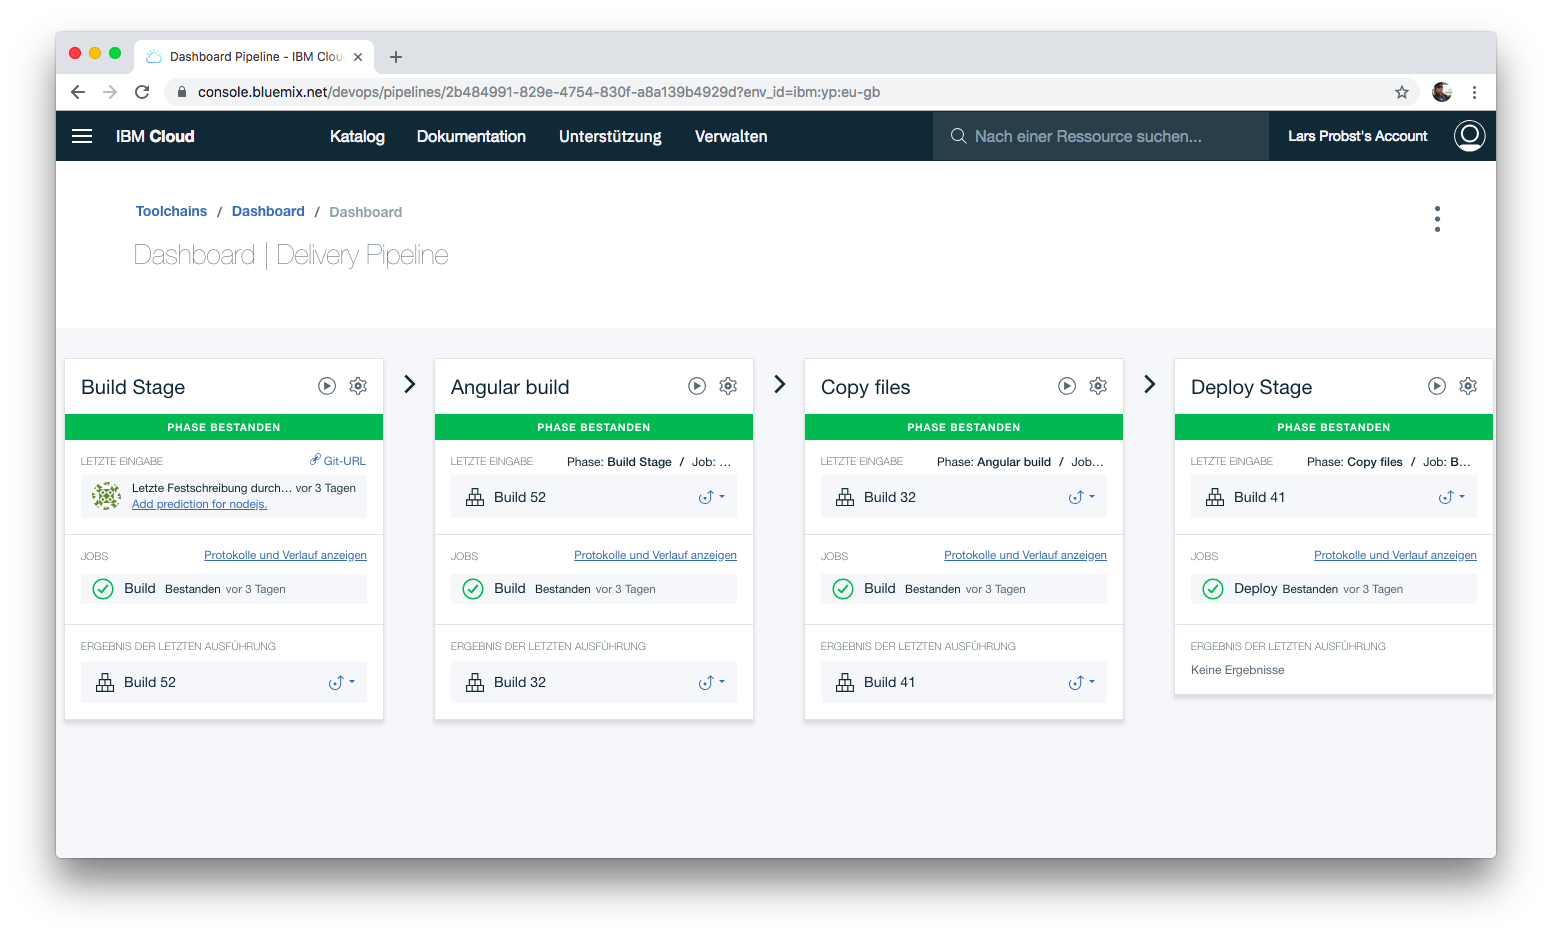
\includegraphics[width=\textwidth]{images/kapitel_3/toolchain_pipeline.png}
    \caption{Übersicht der Toolchain-Konfiguration}
    \label{fig:umsetzung_toolchain_pipeline}
\end{figure}

Als nächstes muss man den geschriebenen Quellcode der Applikation lediglich noch in das, in der Toolchain hinzugefügte,
Git-Repository einchecken. Die URL für das Repository kann man sich in der Toolchain-Übersicht mit einem Klick auf die
Kachel \texttt{Git} anzeigen.

Nach erfolgreichem \texttt{push} der Anwendung in das Git-Repository startet der Deploymentvorgang in der Toolchain
selbstständig. Nach wenigen Minuten ist die Anwendung über ihre URL, welche in der Node.js Runtime definiert ist,
aufrufbar.

Da die Applikation nun im Internet in einem Cloud Foundry-Container zur Verfügung steht, kann diese im nächsten Schritt
mit dem API Connect Service verbunden werden.

Dieser Schritt ist nötig, damit die Schnittstelle der Applikation vom Frontend, welches in Kapitel~\ref{subsec:webseite}
auf Seite~\pageref{subsec:webseite} beschrieben wird, und auch über Postman vereinfacht aufgerufen werden kann.

\subsection{API Connect}
\label{subsec:apiconnect}
Wie in Kapitel~\ref{subsec:Aufruf mit Postman} auf Seite~\pageref{subsec:Aufruf mit Postman} beschrieben, benötigt das
REST-Interface des erstellten Deployments einen Auth-Token. Dieser kann nur über den Aufruf einer anderen
REST-Schnittstelle zur Verfügung gestellt werden.

Damit man diese Schritte vereinfachen kann und das im weiteren Verlauf erstellte Frontend ebenfalls das Deployment aufrufen
kann, werden beide Abfragen in API Connect gebündelt.

Ein weiterer Grund für das Bündeln der beiden Anfragen an den Watson Service ist das Mitschicken des Benutzernamens und
des zugehörigen Passwortes zum generieren des Tokens. Damit diese Daten nicht in der zu entwickelnden Anwendung hinterlegt
werden müssen, kann man diese Zentral in API Connect speichern. Das hat den Vorteil, dass man sie bei Bedarf nur an einer
zentralen Stelle abändern muss.

Desweiteren ist es relativ einfach Daten auszulesen, die von einer Anwendung an die Schnittstelle geschickt werden. Dies
ermöglicht es Angreifern die Daten für andere Zwecke zu missbrauchen.

Ein weiterer Vorteil für die Nutzung von API Connect ist die Bündelung von mehreren Schnittstellen um Vorhersagen zu
beziehen. Aktuell ist es möglich, die Vorhersage aus dem Deployment des Watson Studio Models zu beziehen oder die
entwickelte Node.js Applikation mit TensorFlow.js zu nutzen.

Mittels API Connect kann man die Aufrufe optimal verteilen oder eigene Routen für eine jeweilige Schnittstelle bauen.
Außerdem kann man Änderungen schnell und kompfortabel in einem Online-Editor anpassen.

Die anpassung der Routen in API Connect bedürfen keinerlei Programmierkenntnisse uns sind sehr schnell umgesetzt und in
Echtzeit veröffentlich.

\subsubsection{API Connect einrichten}
Der in Kapitel~\ref{subsec:vorbereitung_apiconnect} auf Seite~\pageref{subsec:vorbereitung_apiconnect} instanziierte
Service wird im folgenden konfiguriert und eingerichtet. Dazu muss man ihn aus dem IBM Cloud Dashboard heraus aufrufen.
Nach dem Klick auf den Service-Namen erscheint eine Seite mit hilfreichen Informationen zum Service.

Über die Schaltfläche \texttt{Open API Connect} gelangt man auf das API Connect Dashboard. In diesem muss man zuerst ein
automatisch angelegten Katalog benennen. In diesem Katalog werden alle Informationen zur API gespeichert.

Veröffentlichte APIs werden automatisch in diesem Katalog aufgelistet. Nach der fertigen Einrichtung des Kataloges gelangt
man über einen Klick auf \texttt{Entwürfe} auf die Entwurfsübersicht.

In dieser muss man den Menüpunkt \texttt{APIs} auswählen. In der erscheinenden Liste werden alle APIs, welche im Weiteren
erstellt werden, aufgelistet. Aktuell existieren hier aber noch keine. Dies kann der Nutzer über den Button
\texttt{Hinzufügen} und dann \texttt{Neue API} ändern.

Nachdem man den Titel, einen Namen und eine beliebige Version hinterlegt hat, kann man die API mit \texttt{API erstellen}
in die Liste aufnehmen. Sie erscheint nun mit dem definierten Namen. Über einen Klick auf diesen lässt sich die
Konfiguration der API öffnen.

Für die Konfiguration einer API existieren drei wichtige Untermenüs. In \texttt{Gestalten} lassen sich Name, Beschreibung,
Version, die Sicherheitsdefinitionen sowie die zur Verfügung gestellten Pfade und dafür vorgesehene Parameter definieren.

Der Menüpunkt \texttt{Quelle} zeigt die komplette Konfiguration der API in Swagger-Notation an. Hier getätigte Änderungen
werden automatisch in den anderen beiden Menüpunkten übernommen.

Im letzten Menüpunkt, \texttt{Assemblieren}, kann man die Funktionen der API definieren. Dazu zählen zum Beispiel die
einzelnen Schritte, welche bei einem Endpunkt durchlaufen werden müssen. Hier wird der Inhalt der API definiert.

Um mit der Konfiguration zu starten, muss der Nutzer zuallererst die einzelnen Pfade, welche zur Verfügung stehen sollen,
definieren. Dazu wird in den Menüpunkt \texttt{Gestalten} gewechselt und im linken Menü dann in \texttt{Pfade}.

Über das kleine Plus-Zeichen im rechten Bereich kann der Nutzer einen neuen Pfad hinzufügen. Pfade sind die Endpunkte
einer REST-Schnittstelle. Jede URL ist ein Endpunkt. Über jeden einzelnen Endpunkt können verschiedene HTTP-Requests
angesteuert werden. Die häufigsten sind \textit{GET}, \textit{POST}, \textit{PUT} und \textit{DELETE}.

Direkt nach einem Klick auf das Plus-Zeichen erscheint ein neuer Pfad mit dem Namen \textit{/pfad-1}. Diesen kann man
durch einen Klick aufklappen. Es erscheinen nun die Konfigurationsparameter für den Endpunkt. Als \textit{Pfad} wird nun
ein Name vergeben, über den das Watson Studio Deployment aufgerufen werden kann. Ein Beispiel hierfür ist
\textit{predict-watson}.

Da in der jetzigen Version für die Parameter keine Validierung vorgenommen wird, kann die Einstellung dieser ignoriert
werden. Allerdings muss man nun eine neue Operation hinzufügen. Dabei handelt es sich um die HTTP-Typen. Da von der
späteren Anwendung Daten an die Schnittstelle geschickt werden sollen, muss es eine Operation vom Typ \textit{POST} sein.

Über den Button \texttt{Operation hinzufügen} kann man diese hinzufügen. In dem Dropdown-Menü muss der Nutzer dann den
entsprechenden \texttt{POST}-Eintrag auswählen. Dieser erscheint sogleich in der Liste und wird grün hinterlegt.

Mit einem Klick auf den \textit{POST}-Eintrag wechselt man in die weitere Konfiguration. Die weitere Konfiguration ist
für die Schnittstelle uninteressant und kann wieder geschlossen werden.

Diese Schritte muss man nun auch für einen weiteren Pfad mit dem Namen \textit{predict-tensorflow} durchführen. Diese
Route ist für die Kommunikation mit der Node.js Applikation notwendig. Sie erhält ebenfalls eine Operation vom Typ
\textit{POST}.

Somit sind erfolgreich zwei Endpunkte mit den Namen \textit{predict-watson} und \textit{predict-tensorflow} angelegt
worden. Diese haben jeweils eine Operation vom Typ \textit{POST}.

Als weitere wichtige Einstellung muss man unter \texttt{Lebenszyklus} den Schalter bei \texttt{CORS} aktivieren und da
im ersten Schritt mit keiner Sicherheit gearbeitet wird, kann der entsprechende Menüpunkt übersprungen werden.

Über das Disketten-Symbol am oberen rechten Rand kann man die aktuelle Einstellung zur Sicherheit speichern. Eine
entsprechende Meldung quittiert die Speicherung.

Die Grundeinstellungen der Schnittstelle sind somit getätigt. Im Weiteren muss der Entwickler die API über
\texttt{Assemblieren} mit dem richtigen Verhalten versehen. Dazu wechselt man über den entsprechenden Menüpunkt in einen
fast leeren Arbeitsbereich.

Hier finden sich im linken Bereich alle möglichen Bausteine um die API mit Funktionen und intelligenz zu füllen. Im
mittleren Teil, dem Arbeitsbereich, ist lediglich ein Punkt hinterlegt. Dieser dient als Einstieg bei einem Aufruf der
Schnittstelle. Ein Aufruf der API landet immer in diesem Knoten und kann dann verteilt werden.

Als einer der ersten Schritte soll die Schnittstelle selbstständig einen Auth-Token vom Watson Studio abgreifen. Dazu
wird das Modul \texttt{Aufrufen} benötigt. Mittels Drag \& Drop kann man dieses Modul in den Arbeitsbereich, direkt
hinter den schon hinterlegten Punkt setzen. Automatisch werden die beiden Module verbunden.

Durch ein doppelten Klick auf das Modul öffnet sich die entsprechende Konfiguration am rechten Bildschirmrand. Als Titel
kann man zum Beispiel \enquote{Get Token} definieren. Als URL dient die Schnittstelle des Watson Studios, welche mit
\enquote{https://eu-gb.ml.cloud.ibm.com/v3/identity/token} angegeben ist.

Der Benutzername und das zugehörige Passwort sind im instanziierten Watson Studio Service zu sehen. Man gelangt über das
IBM Cloud Dashbaord auf die Seite.

Als \textit{HTTP-Methode} muss \texttt{GET} ausgewählt sein. In der Schnittstelle des Watson Studios, existiert auf
diesem Endpunkt lediglich diese Operation.

Als letzte Einstellung muss man als \textit{Antwortobjektvariable} die Bezeichnung \enquote{newtoken} eintragen. Die
Konfiguration des Modules ist damit abgeschlossen und es kann mit den nächsten Modulen fortgefahren werden.

Da die Schnittstelle des Watson Studios den Auth-Token als Rückgabeparameter besitzt, muss man diesen in API Connect
speichern und allgemein zur Verfügung stellen. Dies kann nur über das Modul \texttt{Zuordnen} erfolgen.

Dieses Modul kann man der Kategorie \textit{Umwandlungen} entnehmen und es direkt nach dem Request-Modul platzieren. Es
reiht sich somit dahinter ein. Ein doppelter Klick öffnet die Konfiguration des Modules. Da hier nur ein Parameter
gespeichert werden muss, ist die Konfiguration recht simpel.

In der Spalte Eingabe kann man über den Stift einen neuen Eintrag hinzufügen. Als Kontextvariable ist
\enquote{newtoken.body.token} zu definieren. Dabei handelt es sich um den Rückgabeparameter des vorangestellten
Request-Modules und das JSON-Objekt \enquote{token}, welches von der Schnittstelle zurückgegeben wird.

Als Name der Variable wird \enquote{Token Input} definiert, der Inhaltstyp ist \enquote{text/plain} und die Definition
ist \enquote{string}. Über \texttt{Fertig} kann man die Konfiguration speichern.

Nun muss in der Spalte Ausgabe eine interne Variable definiert werden, welche den Auth-Token speichert. Dafür wird über
den Stift ein neuer Eintrag angelegt. Die Kontextvariable ist \enquote{newtoken} und der Name \enquote{Token Output}.
Als Inhaltstyp wird \enquote{text/plain} ausgewählt, da die Variable auf der Seite der Eingabe als Text definiert ist.
Somit wird auch die Definition auf \enquote{string} gesetzt.

Nachdem auf beiden Seiten nun ein Eintrag erscheint, muss man diese beiden über die rundlichen Punkte verbinden. Eine
grüne Linie symbolisiert anschließend die Verbindung. Die Konfiguration der Zuordnung ist damit fertiggestellt.

Da bei der Schnittstelle mir CORS gearbeitet wird, muss man in einem nächsten Schritt den Header setzen, welche Anfragen
erlaubt sind. Dafür verwendet man einen \textit{Gateway Script}. Dies platziert man einfach hinter dem Zuordnungs-Modul.

Die Konfiguration des Moduls entspricht Quellcode in JavaScript. Die Zeilen in Listing~\ref{ls:umsetzung_cors} auf
Seite~\pageref{ls:umsetzung_cors} definieren die entsprechenden Einstellungen.

\begin{lstlisting}[language=JavaScript, caption=Gateway Script für CORS, label=ls:umsetzung_cors]
// Set CORS headers
apim.setvariable('message.headers.Access-Control-Allow-Origin', '*')
apim.setvariable('message.headers.Access-Control-Allow-Headers', 'Origin, X-Requested-With, Content-Type, Accept')
\end{lstlisting}

Die zweite Zeile besagt, dass die nachfolgende Konfiguration für \textit{alle} Requests zählt, die diese Schnittstelle
aufrufen. Die dritte Zeile besagt, dass die Anfragen akzeptiert werden sollen. Somit kann jede Anwendung mit dieser
Schnittstelle kommunizieren.

Bei einer späteren Konfiguration könnte man Anwendungen, welche auf die Schnittstelle zugreifen können, hier
einschränken. Dazu muss man die IP der Anwendung kennen, welche mit der Schnittstelle kommunizieren möchte. Diese kann
man dann in die zweite Zeile eintragen (das \enquote{*} ersetzen).

Da es zwei Endpunkte für die Schnittstelle geben wird, braucht man nun einen \textit{Operationsswitch}, um je nach
gefordertem Endpunkt auch die richtigen Informationen zurückgeben zu können.

Dieser Switch wird direkt nach dem Gateway Script angeordnet. In der Konfiguration des Switches kann der Nutzer über den
Button \texttt{+ Pfad} einen neuen Zweig hinzufügen. Insgesamt werden zwei Stück benötigt. Der erste Fall ist für
\textit{predict-watson} da. Der Zweite für \textit{predict-tensorflow}.

\subsubsection*{Pfad für das Watson Deployment}
Für den Pfad des \textit{predict-watson} wird ein weiteres Gateway Script benötigt, welches den Header für die Anfrage
an des Watson Studio Deployment setzt. Für die Einstellungen sind die JavaScript Zeilen in
Listing~\ref{ls:umsetzung_settoken} auf Seite~\pageref{ls:umsetzung_settoken} zuständig.

\begin{lstlisting}[language=JavaScript, caption=Gateway Script für den Authorization-Token, label=ls:umsetzung_settoken]
// Set the token
var token = apim.getvariable('newtoken');
apim.setvariable('message.headers.authorization', 'Bearer' + token);
\end{lstlisting}

In der zweiten Zeile wird der Token, welcher in dem Modul \textit{Zuordnung} gespeichert wurde, ausgelesen. Die dritte
Zeile sorgt dafür, dass ein Header mit dem Key \textit{authorization} und dem Value \textit{Bearer + token} gesetzt wird.

Diese Einstellungen sind wichtig, damit der spätere Request an das Watson Studio Deployment die richtigen Benutzerdaten
erhält um die Anfrage für gültig zu erklären.

Ein weiteres Gateway Script sorgt dafür, dass die ursprünglich übergebenen Parameter an den API Connect Service (mit den
Input-Werten für die Vorhersage) auch an den nächsten Request weitergegeben werden können.

Dafür setzt man die alten Werte als neue Message-Werte. Das Listing~\ref{ls:umsetzung_header} auf
Seite~\pageref{ls:umsetzung_header} veranschaulicht das vorgehen.

\begin{lstlisting}[language=JavaScript, caption=Gateway Script zum Setzen des Message-Bodys, label=ls:umsetzung_header]
// Get variables
var request = apim.getvariable('request.body');
apim.setvariable('message.body', request);
\end{lstlisting}

Im letzten Schritt muss man ein weiteres Aufruf-Modul hinzufügen. Dies erledigt den eigentlichen Aufruf an das Watson
Studio Deployment. Dazu wird das Modul als das Nächste in die Reihe eingefügt. In der Konfiguration muss man lediglich
die URL des Deployments hinzufügen. Diese ist auf der Seite des Deployments ersichtlich.

Damit ist dieser Pfad fertig konfiguriert und kann mit einem Aufruf verifiziert werden. Im nächsten Schritt wird der
zweite Pfad eingerichtet.

\subsubsection*{Pfad für den TensorFlow Container}
Die Einrichtung des TensorFlow-Pfades ist sehr ähnlich zum vorherigen Pfad. Allerdings bedarf es keines Gateway Scriptes
zum setzen eines Authorization Tokens, da dieser hier nicht benötigt wird. Die anderen Module kann man kopieren und in
dem Pfad einsetzen. Lediglich das Aufrufen-Modul benötigt weitere Konfiguration.

In diesem muss nicht die URL des Watson Studio Deployments definiert sein, sondern man muss die des Cloud
Foundry-Containers einsetzen. Anschließend sollte man die Konfiguration über das Disketten-Symbol speichern.

Die Konfiguration des API Conenct Services ist somit abgeschlossen und man kann diese im eingerichteten Katalog
veröffentlichen.

\subsubsection{API Veröffentlichen}
In der Abbildung~\ref{fig:umsetzung_api_connect} auf Seite~\pageref{fig:umsetzung_api_connect} ist der fertig eingerichtete
API Connect Flow dargestellt. Dieser umfasst alle notwendigen Module und Einstellungen.

\begin{figure}[h]
    \centering
    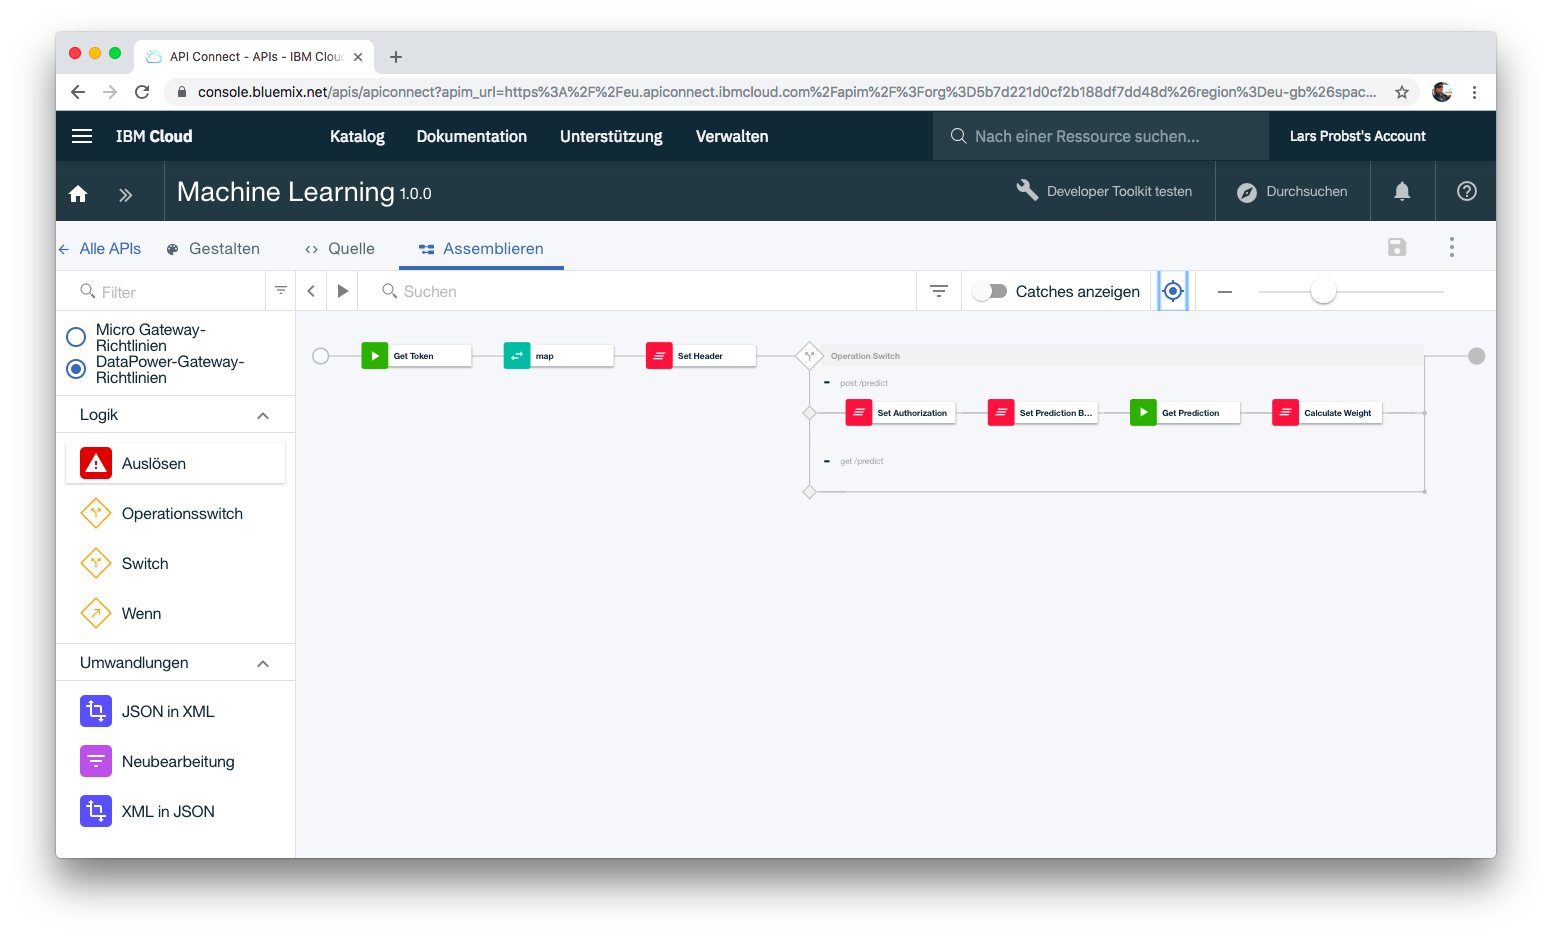
\includegraphics[width=\textwidth]{images/kapitel_3/api_connect.png}
    \caption{Kompletter API Connect Flow}
    \label{fig:umsetzung_api_connect}
\end{figure}

Über den Play-Button am linken oberen Rand, kann man die aktuelle Konfiguration des API Connect Services bauen lassen.
Als Katalog sollte man den anfangs angelegten Katalog definieren. Im Bereich Produkt muss der Nutzer ein Neues anlegen.

Bei dem Produkt handelt es sich um einen Namen für den Service. Die API läuft später unter diesem Produkt-Namen und kann
in dem anfangs erstellten Katalog über das Produkt gefunden werden.

So ist es möglich mehrere APIs für einen Produkt zu definieren. Ein Endnutzer kann sich ein Produkt dann über den Katalog
beziehen und die angelegte API nutzen.

Nun kann man mit \texttt{Produkt veröffentlichen} dieses veröffentlichen und nutzbar machen. Dieser Vorgang kann bis zu
wenigen Minuten dauern.

\subsubsection{API durchsuchen}
Auf dem API Connect Dashboard kann der Benutzer über die rechts oben angelegte Schaltfläche \texttt{Durchsuchen} auf ein
Untermenü zugreifen. In diesem werden alle Kataloge und Entwürfe aufgelistet, die durch ihn erstellt wurden.

Mit einem Klick auf den ersten Eintrag in der Kategorie \textit{Katalog} gelangt man auf eine Übersicht aller
API-Endpunkte, welche sich in diesem Katalog befinden.

Aktuell sollten im linken Feld lediglich zwei Endpunkte zu sehen sein. Der Endpunkt \textit{predict-watson} für das
Watson-Deployment und der Endpunkt \textit{predict-tensorflow} für den Node.js Wrapper. Auch sollten beide über
den HTTP-Type \textit{POST} definiert sein.

Außerdem könnte in diesem Bereich nach einem Endpunkt gesucht oder die Endpunkte sortiert werden. Jeder Eintrag in der Liste
kann angeklickt werden. Daraufhin wird die mittlere Ansicht, in der Informationen zum Endpunkt stehen, zu der jeweiligen
Stelle gescrollt.

Auch kann man der mittleren Spalte für jeden Endpunkt Informationen zu den verwendeten und produzierten Datentypen
entnehmen. Diese Informationen können bei der Konfiguration des API-Endpunktes angegeben werden. Dies ist in
Kapitel~\ref{subsec:apiconnect} auf Seite~\pageref{subsec:apiconnect} erklärt.

Jede zusätzliche Information, die bei der Konfiguration eingetragen wird, erweitert die Ansicht des mittleren Bereiches
um die jeweilige Informationen.

Im rechten Bereich der Ansicht werden Beispielaufrufe angezeigt, wie man die jeweiligen Endpunkte zum Beispiel mit dem
Befehlsprogramm \textit{curl} aufrufen kann. Dies ist hilfreich um die Endpunkte zu testen oder in Erfahrung zu bringen,
wie die Rückgabewerte aussehen.

Außerdem kann man sich die Aufrufe mit anderen Programmiersprachen anschauen. Dies erleichtert die Entwicklung und
Einbindung der Schnittstelle in eigene Programme erheblich.

Als letzte Funktion kann man im rechten Bereich die API-Endpunkte auch direkt online testen. Dies ist hilfreich um die
Funktion des Endpunktes zu überprüfen ohne ein externes Tool nutzen zu müssen.

Bei der Ansicht handelt es sich um eine Darstellung der automatisch generierten Konfigurationsdatei (\textit{yaml}-Datei)
mit einer Swagger-UI\footnote{https://swagger.io/tools/swagger-ui}, welche von IBM optisch angepasst wurde.

\subsubsection{Developer Toolkit}
Ebenfalls über das API Connect Dashboard kann der Entwickler auf den Menüpunkt \texttt{Developer Toolkit} zugreifen.
Dieser zeigt eine Anleitung, wie man die erstellte API auf einem eigenen Server einrichten kann. Dafür sind lediglich
drei einfache Schritte notwendig.

Zuallererst muss man das Programm \textit{API Connect} mittels npm herunterladen und installieren. Anschließens wird über
die Funktion \textit{loopback} eine neue API auf dem lokalen API Connect Service eingerichtet. Der Wizzard führt einen
durch die benötigte Konfiguration.

Nun kann man die Web-Oberfläche des lokalen API Connect starten und seine erstellte, noch leere API, sehen. Anschließend
muss man nur noch die Konfigurations-Datei der online erstellten API kopieren und in den lokalen Service einfügen.

Über den Menüpunkt \texttt{Run Your API}, gelangt man auf eine weitere Anleitung, welche das starten und zur Verfügung
stellen der lokal erstellten API erläutert.

Im letzten Schritt, welchen man über die Schaltfläche \texttt{Publish Your API to IBM Cloud} erreicht, wird Schritt für
Schritt erklärt, wie man die lokal erstellte API nun wieder in der IBM Cloud im Service Watson Studio verfügbar machen
kann.

Dies ist dann sinnvoll, wenn man lokal Änderungen vorgenommen hat und diese wieder online einspielen möchte.

Nach einem Neustart des lokalen Services kann die API genutzt werden und man ist nicht mehr auf eine Cloud-Lösung
angewiesen.

Dies kann diverse Vorteile für die Erstellung einer eigenen Architektur haben. Gerade wenn Applikationen lediglich im
internen Netz zur Verfügung stehen, man allerdings den API Connect Service nutzen möchte.

Oder zum offline Erstellen einer API, da bei der Entwicklung nicht immer eine Verbindung zu den IBM Servern gewährleistet
werden kann.

Eine detailliertere Anleitung steht auf der geöffneten Webseite zur Verfügung. Dort kann man sich die einzelnen Befehle
und Kommandos direkt herauskopieren um diese ausführen.
\section{Abschluss}
Das neuronale Netz ist an dieser Stelle fertig trainiert und erfolgreich als Modell exportiert. Auch kann man es als
Deployment über einen Webdienst aufrufen und Vorhersagen triggern.

Mittels internem Onlinetest und über das externe Programm \textit{Postman} wurde der Aufruf des Webdienstes überprüft
und die Parameter verifiziert.

Desweiteren ist das trainierte Modell erfolgreich in einen Node.js Wrapper eingebaut, der eine TensorFlow.js
Anwendung beherbergt. Diese Anwendung lädt beim Ausführen das aktuelle Modell in den Speicher und parametriesiert es
mit den Eingabevariablen.

Nach kurzer Zeit werden die vorhergesagten Parameter als Rückgabewert über den Request zurückgegeben und eine Anfrage
wurde so erfolgreich durchgeführt.

Sowohl der Webdienst als auch der Node.js Wrapper sind in einem API-Gateway vereint, sodass Aufrufe an die beiden
Endpunkte vereinfacht werden können. Auch Authentifizierung und Sicherheitsmechanismen laufen über den API-Gateway um
eine Anpassung zu vereinfachen.

Um dem Endnutzer eine vereinfachte Möglichkeit zu bieten, Anfragen an die beiden Vorhersagemodelle zu schicken, wird
im nächsten Schritt ein Frontend dafür eingerichtet. Mit diesem ist es Möglich die Inputs für die Bosch KWE einzugeben
und die vorhergesagten Parameter schön darzustellen.

Außerdem ist so ein Test der komplette Architektur mit Webdienst, Node.js Wrapper mit integrierter TensorFlow.js
Applikation und API Connect möglich.

Denn über das Frontend soll ein Request an den API-Gateway gesendet werden, welcher dann weiter an ein Vorhersagemodell
geschickt wird. Die Antwort des Modells gelangt dann zurück zum API-Gateway und dann wieder zurück an das Frontend.

In einem Aufruf sind alle bisher gebauten Komponenten involviert, sodass durch einen Test das Zusammenspiel der
Kommunikation der einzelnen Komponenten möglich ist.

Die dafür notwendige Umsetzung wird in Kapitel~\ref{ch:client} ab Seite~\pageref{ch:client} behandelt und Schritt für
Schritt realisiert.
\chapter{Client}
\label{ch:client}
Das nachfolgende Kapitel beschreibt die Entwicklung einer Applikation, dem Client, welches die in
Kapitel~\ref{ch:neuronalesNetz} ab Seite~\pageref{ch:neuronalesNetz} implementierte Architektur nutzt, um Anfragen an
die neuronalen Netze für den Endnutzer einfacher zu gestalten.

Dabei ist die Anwendung für die Eingabe der benötigten Parameter zuständig und das Abfangen von falsch eingetragenen
Werten in das dargestellte Formular. Anschließend überträgt der Client die eingetragenen Werte an die neuronalen Netze
und stellt die Vorhersagen aufbereitet dar.

Die Architektur beherbergt zwar zwei Anwendungen mit jeweils einem Endpunkt, allerdings sind diese gemeinsam über
den API Connect Service aufrufbar. Dies erleichtert die Entwicklung des Clients dahingehend, dass lediglich eine
Kommunikation zwischen der neuen Applikation und dem Bluemix-Service notwendig ist.

Da, wie in~\cite{online_client_apps} zu lesen, Smartphone-Apps eine immer wichtigere Rolle im Leben eines Endnutzers
spielen, soll neben einer Webanwendung (englisch Frontend) auch für die beiden größten Hersteller von
Smartphone-Betriebssystemen eine App entstehen. Somit soll ein noch viel größerer Kundenbereich abgedekt werden.

Das Frontend soll in einem Container laufen um ihn möglichst schnell und komfortabel sowohl in der Cloud als auch 
im eigenen Rechenzentrum betreiben zu können. Die Abbilung~\ref{fig:schematische_architektur_4} auf
Seite~\pageref{fig:schematische_architektur_4} zeigt die schematische Architektur des Frontends mit den ausgehenden
Verbindungen mit den Anfragen.

Die notwenigen Schritte für den Aufbau eines Containers sollen in einem Continuous Deployment verankert werden, um sie
möglichst modular zu halten.

\begin{figure}[h]
    \centering
    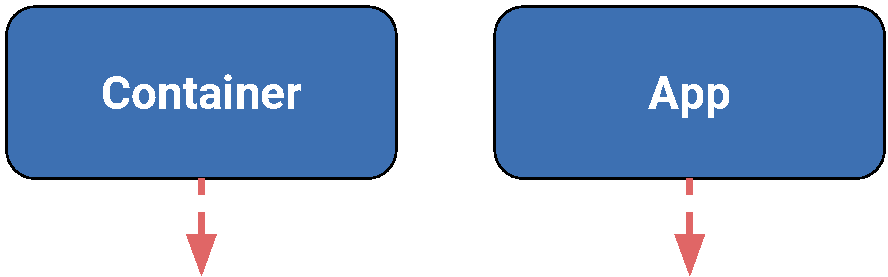
\includegraphics[scale=0.5]{images/kapitel_4/architektur_schematisch.pdf}
    \caption{Schematische Darstellung der Architektur}
    \label{fig:schematische_architektur_4}
\end{figure}
\section{Analyse}
Dieses Kapitel soll verschiedene Umsetzungsmöglichkeiten für die Webseite als auch für die Smartphone-Apps analysieren
und eine Einleitung für die präferierte Möglichkeit geben.

Ziel ist es für sowohl die Webseite als auch für die Smartphone-Apps eine optimale Möglichkeit zu finden, diese
umzusetzen, zu verwalten und in Betrieb zu nehmen.

Mit den Ergebnissen wird in den darauffolgenden Kapiteln fortgesetzt und sie werden Schritt für Schritt umgesetzt.

%% TODO noch schreiben
\subsection{Webseite}
Wir könnten eine Webseite aufbauen. Am besten responsive.

\colorbox{yellow}{Hier fehlt was}

%% TODO noch schreiben
\subsection{App}
Wir könnten aber auch eine Native App bauen, mit der wir alles darstellen.

\colorbox{yellow}{Hier fehlt was}

%% TODO noch schreiben
\subsection{Hybrid}
Wie könnten wir das noch machen? WebViewer-App? Also eine Mischung aus beidem.

\colorbox{yellow}{Hier fehlt was}
\section{Vorbereitung}
Damit im Weiteren das Frontend und die Smartphone-Apps entwickelt und gebaut werden können, werden drei Programme auf
dem Entwicklungsrechner installiert und ein Service in der IBM Cloud instanziiert sowie eingerichtet und verwaltet.

Die Vorgehensweise wird in den folgenden Kapiteln erläutert und Schritt für Schritt erklärt.

\subsection{Angular CLI}
Für die Erstellung, die Verwaltung und die Aktualisierung einer Angular-Applikation empfiehlt es sich, das hauseigene
Command Line Interface (CLI) zu nutzen. Über den folgenden Befehl wird dieses auf einem Linux oder macOS Rechner
installiert.

\begin{lstlisting}[caption=Installation des Angular CLI, label=ls:vorbereitung_angularcli]
    $ npm install -g @angular/cli
\end{lstlisting}

Anschließend steht die Applikation über das Kommando \texttt{ng} zur Verfügung. Dies ist eine Abkürzung für
\textit{A\textbf{ng}ular}.

\subsection{Android Studio}
Für die Entwicklung einer Android-App stehen zahlreiche Tools zur Verfügung. Eines der bekanntesten ist das Android
Studio. Bei diesem Programm handelt es sich um eine IDE auf Basis von IntelliJ Community
Edition\footnote{https://www.jetbrains.com/idea} und ist kostenlos.

Die Installation von Android Studio erfolgt durch das Herunterladen des jeweiligen Installationspaketes auf der
Installationsseite\footnote{https://developer.android.com/studio/install}.

Nach erfolgreicher Installation kann man die IDE zum ersten Mal starten und ein neues Projekt anlegen.

\subsection{Xcode}
iOS-Apps kann man lediglich durch das Apple eigene Xcode entwickeln. Die Installation kann nur auf einem macOS
erfolgen und dort durch den App Store\footnote{https://itunes.apple.com/de/app/xcode/id497799835}.

Nach erfolgreicher Installation erscheint die IDE im Dock und ist bereit zur Nutzung.

\subsection{Node.js Runtime}
Damit man das erstellte Frontend online aufgerufen kann wird in der IBM Cloud eine zusätzliche Node.js Runtime
benötigt.

Genau wie in Kapitel~\ref{ssc:nodejs_runtime} auf Seite~\pageref{ssc:nodejs_runtime} beschrieben ist die Einrichtung
und Konfiguration einer solchen Runtime über den folgenden Befehl möglich:

\begin{lstlisting}[caption=Instanziierung der Node.js Runtime, label=ls:vorbereitung_nodejsdashboard]
    $ ibmcloud cf create-service nodejs service_name
\end{lstlisting}

Anschließend steht die Runtime in der Kategorie \textit{Cloud Foundry-Anwendungen} im IBM Cloud Dashboard zur Verfügung,
und man kann sie nutzen.

\section{Umsetzung}
Das Architekturbild~\ref{fig:umsetzung_frontendarchitektur_4} auf Seite~\pageref{fig:umsetzung_frontendarchitektur_4}
zeigt die Architektur des Frontends und die Kommunikation mit dem API Connect Service. Dabei sollen sowohl das Frontend
als auch die Smartphone-Apps mit dem API Gateway kommunizieren, um die Anfragen zu vereinheitlichen.

Ein Cloud Foundry-Container wird mit einem Node.js-Boilerplate versehen. Mit Hilfe des Boilerplates lassen sich
Node.js-Applikationen innerhalb des Containerts verwalten und nutzen. Es stellt eine Runtime zur Verfügung, in welcher
das Frontend laufen kann.

Die Smartphone-Apps werden auf Basis von Android und auch iOS entwickelt. Beide Systeme erhalten innerhalb der App ein
WebView-Layout, welche für das Laden und das Darstellen der Webseite zuständig ist. Damit ist es einfach, eine schon
erstellte, responsive Webseite optimal für ein Smartphone zu nutzen. Zusätzlich können Feinheiten wie angepasste Layouts
der einzelnen Systeme übernommen werden.

Die Kommunikation zwischen Frontend und API Connect sowie zwischen den entwickelten Smartphone-Apps und dem API Connect
Service laufen über REST-Aufrufe (englisch REST-Calls).

Da in den Smartphone-Apps lediglich das schon geschriebene Frontend geladen wird, müssen die Aufrufe nur ein Mal
spezifiziert und umgesetzt werden.

\begin{figure}[h]
    \centering
    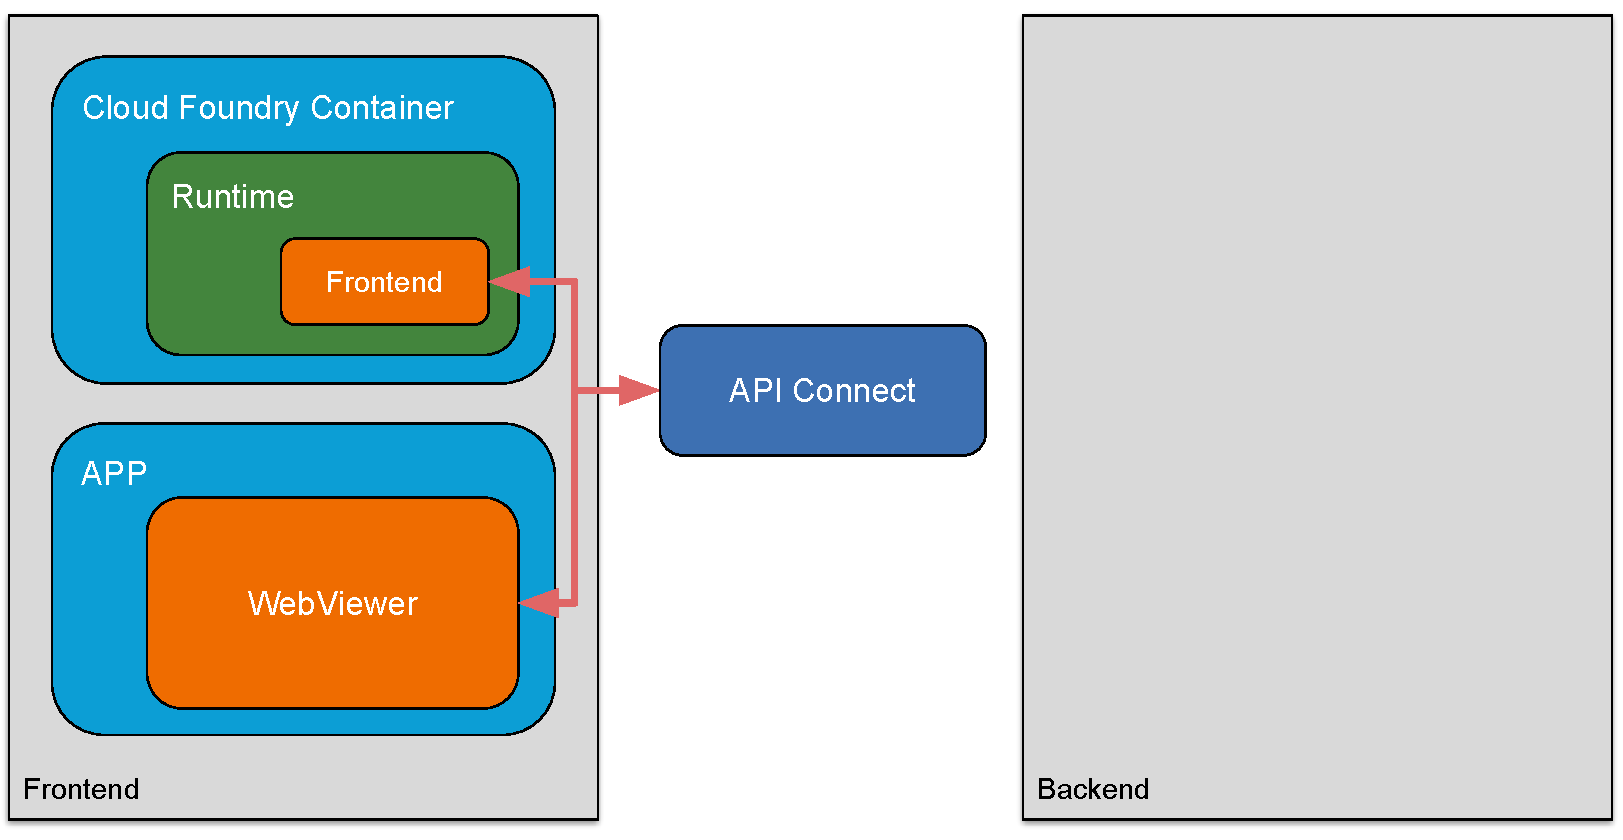
\includegraphics[width=\textwidth]{images/kapitel_4/architektur_frontend.pdf}
    \caption{Übersicht der Zielarchitektur}
    \label{fig:umsetzung_frontendarchitektur_4}
\end{figure}

\subsection{Web-Frontend}
\label{subsec:webseite}
Als nächstes kann man das Web-Frontend (auch Webseite oder englisch website oder auch client genannt) entwickeln. Um
nicht mit zahlreiche Iterationen und Anpassungen bei der Entwicklung zu kämpfen, empfiehlt es sich mit der Definition
von Use-Cases -- also mit der Definition der Aktionen eines Endnutzers auf der Webseite -- zu beginnen.

Anschließend sollte man für die einzelnen Use-Cases Mockups erstellen, die aufzeigen, wie ein Endnutzer die einzelnen
Aktionen durchführen kann. In einem weiteren Schritt setzt der Entwickler die gebauten Mockups dann in Quellcode um,
damit ein Prototyp enstehen kann. Diesen könnte man dann mit einer ausgewählten Gruppe testen.

Damit die Benutzung der Webseite von verschiedenen Endgeräten aus möglich ist, muss man sich im Weiteren gedanken über
das Thema \textit{Responsive} machen. Wie sich die gebaute Webseite also auf den verschiedenen Displaygrößen anpasst.

Nachdem man die Webseite dann fertig entwickelt hat, muss man sie noch in einen Container installieren. Dies ist über
mehrere Varianten möglich. Auch kann man zusätzliche Erweiterungen einbauen, welche das Arbeiten mit der Webseite
erleichtern oder speziellen Bedürfnissen der Endanwender gerecht wird.

\subsubsection{Use-Cases}
Als Use-Case kommt zum jetzigen Zeitpunkt lediglich eine Aktion in Frage. Das Erstellen von Vorhersagen für die
manuell eingetragenen Parameter der Maschine.

Da das Backend mit seinem neuronalen Netz aktuell nicht mehr berechnen kann, ist der angegebene Use-Case auch der einzig
sinnvolle.

Nachdem der Endnutzer die Parameter dann in das Formular eingetragen hat, soll er die Möglichkeit bekommen, die
resultierenden Vorhersagen zu erhalten, um diese an der Maschine zu testen. Eine Fortschrittsanzeige soll darüber
informieren, dass das System arbeitet.

Da der Use-Case relativ einfach definiert werden konnte, kann man als nächstes mit der Erstellung der Mockups beginnen,
um eine erste Idee der Anwendung und ihrem Aussehen zu bekommen.

\subsubsection{Mockups erstellen}
Da der Use-Case nun definiert ist, kann man mit der Entwicklung der Mockups beginnen. Dabei ist die Wahl des Designs auf
eine zweispaltige Startseite gefallen. Eine der beiden Spalten beinhlatet die Eingabewerte und die andere Spalte
beinhaltet die vorhergesagten Argumente, welche von dem neuronalen Netz bestimmt werden.

In Abbildung~~\ref{fig:umsetzung_mockup_scale_1} auf Seite~\pageref{fig:umsetzung_mockup_scale_1} zeigt eine erste
Version des Frontends zur Umsetzung der beiden Spalten. Dabei werden in der linken Spalte die Werte in Formularfelder
eingetragen und in der rechten Spalte die vorhergesagten Parameter angezeigt.

Im mittleren Bereich der Seite soll ein Button erscheinen, welcher durch betätigen die eingetragenen Parameter an das
Backend schickt und anschließend den Output anzeigt.

\begin{figure}[h]
    \centering
    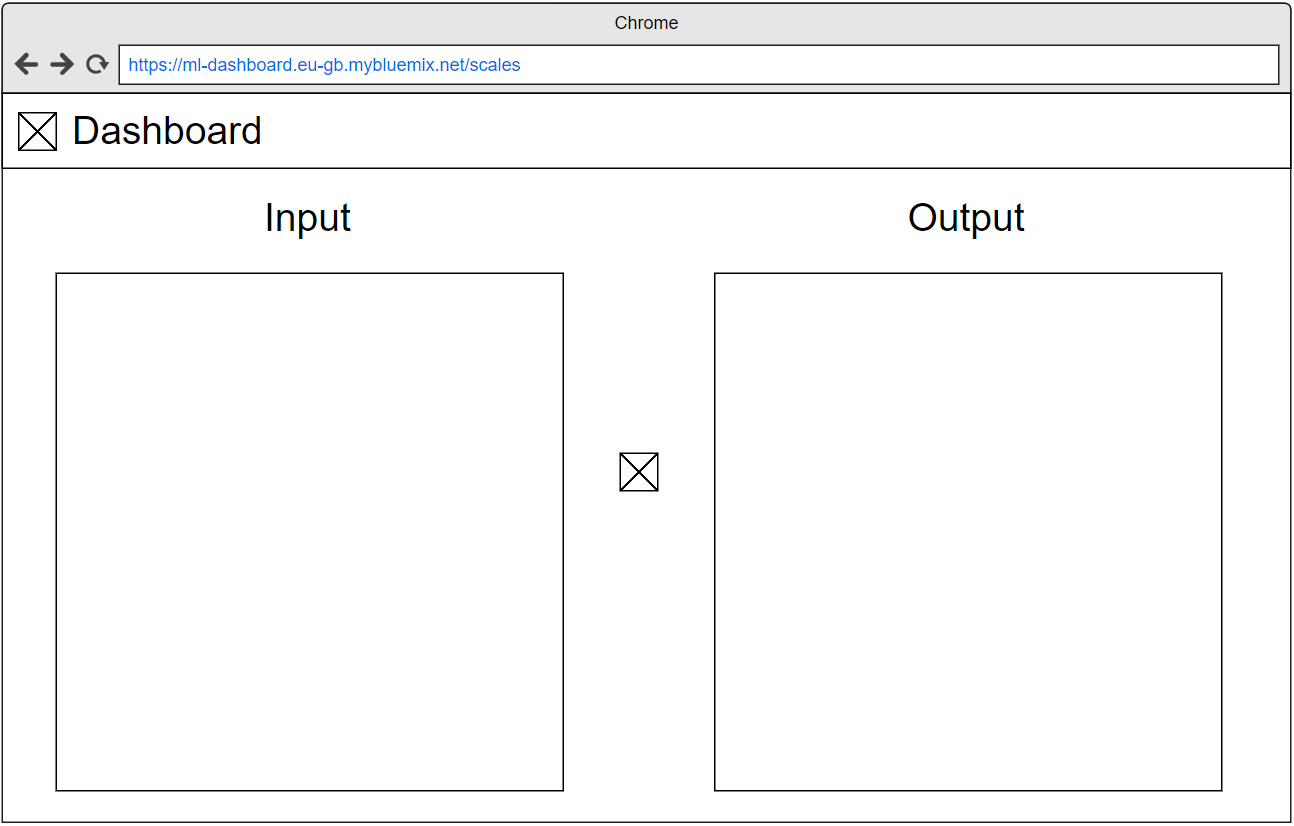
\includegraphics[width=\textwidth]{images/kapitel_4/mockup_scale_1.png}
    \caption{Erstes Mockup für das Dashboard}
    \label{fig:umsetzung_mockup_scale_1}
\end{figure}

Damit man sowohl der Input als auch der Output verbessert anzeigen kann ist es sinnvoll, die beiden Spalten noch weiter
zu unterteilen. Gerade bei den Eingabewerten gibt es zahlreiche Parameter, die in Gruppen zusammengefügt werden können.

So ist es zum Beispiel möglich die Parameter \textit{Produktbreite}, \textit{Produkthöhe} und \textit{Produkttiefe} zu
einer Gruppe namens \textit{Produktmaße} zusammenzufügen.

Die Abbildung~\ref{fig:umsetzung_mockup_scale_2} auf Seite~\pageref{fig:umsetzung_mockup_scale_2} zeigt das angepasste
Mockup mit seinen Gruppen sowohl auf der Input"~ als auch der Output-Seite.

\begin{figure}[h]
    \centering
    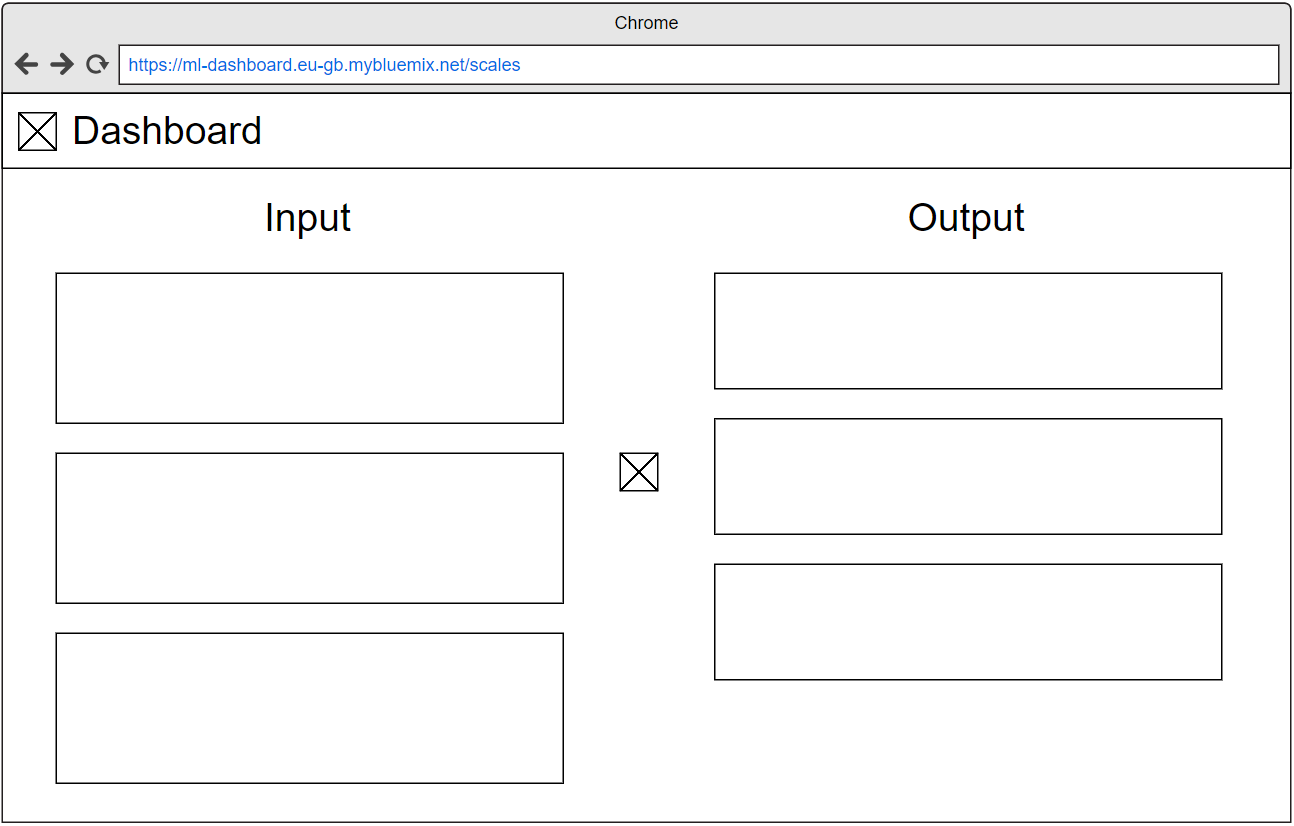
\includegraphics[width=\textwidth]{images/kapitel_4/mockup_scale_2.png}
    \caption{Überarbeitetes Mockup für das Dashboard}
    \label{fig:umsetzung_mockup_scale_2}
\end{figure}

Im oberen Bereich der Anwendung kann man ein Logo der Anwendung erscheinen lassen und nebenan den Namen für die aktuell
geöffnete Seite.

Damit man das Frontend auch für weitere Maschinen oder Maschinenkomponenten anpassen kann, kann der Entwickler ein Menü
hinzufügen, über das man auf die anderen Seiten mit Eingabe"~ und Ausgabewerte zugreifen kann.

Dieses Menü entwickelt man am Besten so, dass es sich aus dem linken Bereich herausschiebt und über ein
\textit{Hamburger-Menü-Icon}\footnote{https://de.wikipedia.org/wiki/Hamburger-Menü-Icon} zu öffnen ist.

So ist in Abbildung~\ref{fig:umsetzung_mockup_scale_menu} auf Seite~\pageref{fig:umsetzung_mockup_scale_menu} das Mockup
für ein seitliches Menü zu sehen, welches über drei beispielhafte Menüeinträge verfügt.

Das Menü soll sich beim aufklappen über den Inhalt legen und den restlichen Bildschirm etwas ausgrauen, sodass für den
Nutzer ersichtlich ist, dass aktuell am Menü eine Auswahl getroffen werden muss.

Ein Klick in den ausgegrauten Bereich, oder auch auf einen der Menüpunkte, schließt das Menü allerdings wieder, sodass
der Nutzer immer das tun kann, was er gerade möchte.

Die Auswahl eines neuen Menüpunktes hat außerdem zur Folge, dass sich die vorher angesprochene Überschrift im oberen
Bereich der Webseite mit dem Namen des Menüpunktes füllt, damit der Nutzer immer genau weiß, unter welchem Menüpunkt
er sich aktuell befindet.

\begin{figure}[h]
    \centering
    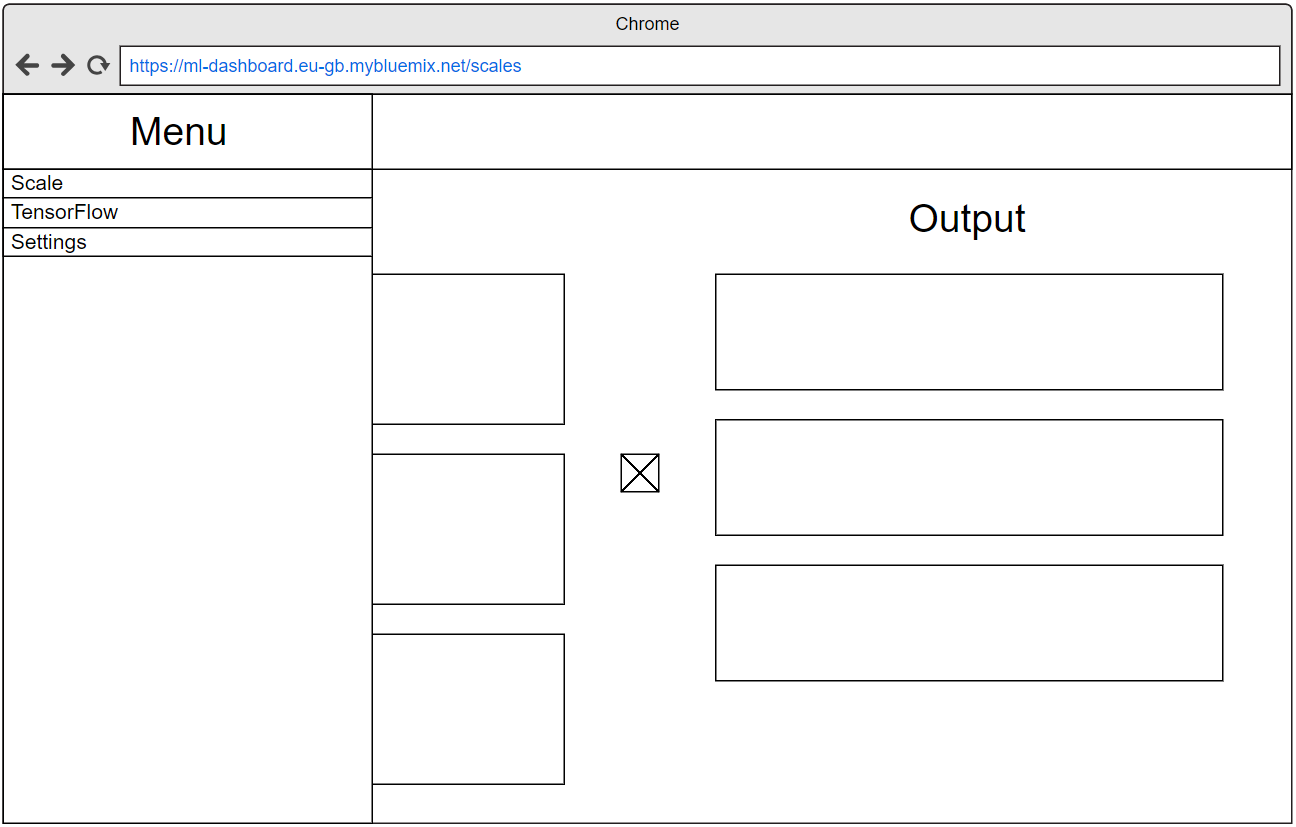
\includegraphics[width=\textwidth]{images/kapitel_4/mockup_scale_menu.png}
    \caption{Mockup für die Navigation}
    \label{fig:umsetzung_mockup_scale_menu}
\end{figure}

\subsubsection{Gedanken zu Responsive}
Damit das Frontend auch von einem Smartphone aus bedient und eine WebView-App dafür geschrieben werden kann, muss die
Webseite auf verschiedene Displaygrößen so reagieren können, damit es alle Informationen nutzerfreundlich anzeigt. Dabei
dürfen keine wichtigen Informationen verschwinden oder die Interaktion mit dem System eingeschränkt sein.

Um dieser Anforderung gerecht zu werden, muss das Frontend mit responsiven Eigenschaften versehen werden. Da die
Webseite in Ihrer ursprünglichen Idee zwei Spalten hat, ist es für die responsive Version interessant, die Spalten nicht
nebeneinander anzuzeigen, sondern untereinander. Dies aber auch nur, sofern es nicht genügend Platz hat, um beide
Spalten nebeneinander anzuzeigen.

Bei größeren Displays wäre es im horizontalen Modus (englisch landscape mode) möglich, beide Spalten auch nebeneinander
anzuzeigen. Wohingegen im vertikalen Modus (englisch portrait mode) immer Sinnvoll ist, die beiden Spalten untereinander
anzuzeigen.

Das Mockup in Abbildung~\ref{fig:umsetzung_mockup_scale_responsive} auf Seite~\pageref{fig:umsetzung_mockup_scale_responsive}
zeigt die Darstellung des Frontends auf einem Smartphone im vertikalen Modus. Dabei ist die Spalte mit der
\textit{Eingabe} aktuell sichtbar und unterhalb wird der Button für die Berechnung der Ausgabeparameter angezeigt.

Unter dem Button ist die Spalte für die Ausgabeparameter angesiedelt, welche erst erscheint, wenn Vorhersagen zur
Verfügung stehen. So ist der Scrollbalken auf der Webseite nicht unnötig lang um den Endnutzer nicht zu verunsichern.

Auch wird nach der Bestätigung des Buttons automatisch zum Bereich der Ausgabe gescrollt, damit dies nicht manuell
geschehen muss.

\begin{figure}[h]
    \centering
    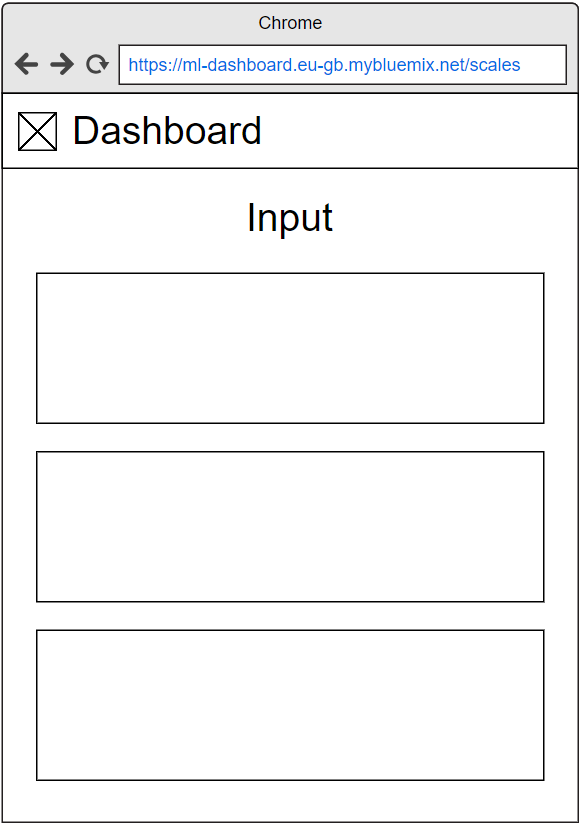
\includegraphics[scale=0.45]{images/kapitel_4/mockup_scale_responsive.png}
    \caption{Mockup des responsiven Designs}
    \label{fig:umsetzung_mockup_scale_responsive}
\end{figure}

\subsubsection{Webseite umsetzen}
Da die Mockups für die Anwendung fertig umgesetzt sind, kann im Weitern damit begonnen werden, das Frontend wirklich
umzusetzen. Da man das Frontend mit Angular umsetzt und die Angular-CLI installiert ist, kann man auf dem
Entwicklerrechner mit dem folgenden Befehl eine neue Angular-Seite einrichten.

\begin{lstlisting}[language=bash, caption=Einrichten einer neuen Angular-Seite, label=ls:umsetzung_angular]
    ng new dashboard
\end{lstlisting}

Dabei wird ein neuer Ordner mit dem Namen \textit{dashboard} angelegt, welcher alle benötigten Ordner und Dateien um
eine funktionierende Angular-Seite zu bauen beinhaltet. Wenn man anschließend in den neu erstellen Ordner wechselt, kann
man mit dem folgenden Befehl die Standard-Applikation von Angular bauen lassen und sie im Browser ansehen.

\begin{lstlisting}[language=bash, caption=Bereitstellen der Angular-Webseite, label=ls:umsetzung_angularserve]
    ng serve --open
\end{lstlisting}

Der Browser öffnet sich automatisch und zeigt die Standardanwendung. Darin ist ein großes Bild des Angular-Logos mit
einer großen Überschrift und ein paar weiteren Kommentaren zu sehen.

Jegliche Änderung am Quellcode der aktuellen Anwendung hat zur Folge, dass die entsprechende Angular-Komponente neu
gebaut und der Browser neu geladen wird um die Änderung direkt sichtbar zu machen.

Nun kann damit begonnen werden, die Webseite entsprechend der Mockups umzusetzen. Dabei ist darauf zu achten, die
Standard-Komponenten der Angular-Material-Bibliothek zu nutzen, damit das Erscheinungsbild der Anwendung einer Android-
App ähnelt.

Die Komponenten sind auf der entsprechenden Dokumentationsseite\footnote{https://material.angular.io/components/categories}
einsehbar und man kann sie von da aus direkt kopiert um sie im eigenen Quellcode zu nutzen. Auch Icons und vorgefertigte
Farben kann man der Webseite entnehmen um eine im Stil passende Webseite zu bauen.

In Abbildung~\ref{fig:umsetzung_website_input} auf Seite~\pageref{fig:umsetzung_website_input} ist die fertige
umgesetzte Webseite zu sehen, welche die Parameter für das neuronale Netz eingeben kann. Die linke Spalte mit der
\textit{Eingabe} ist also umgesetzt.

\begin{figure}[h]
    \centering
    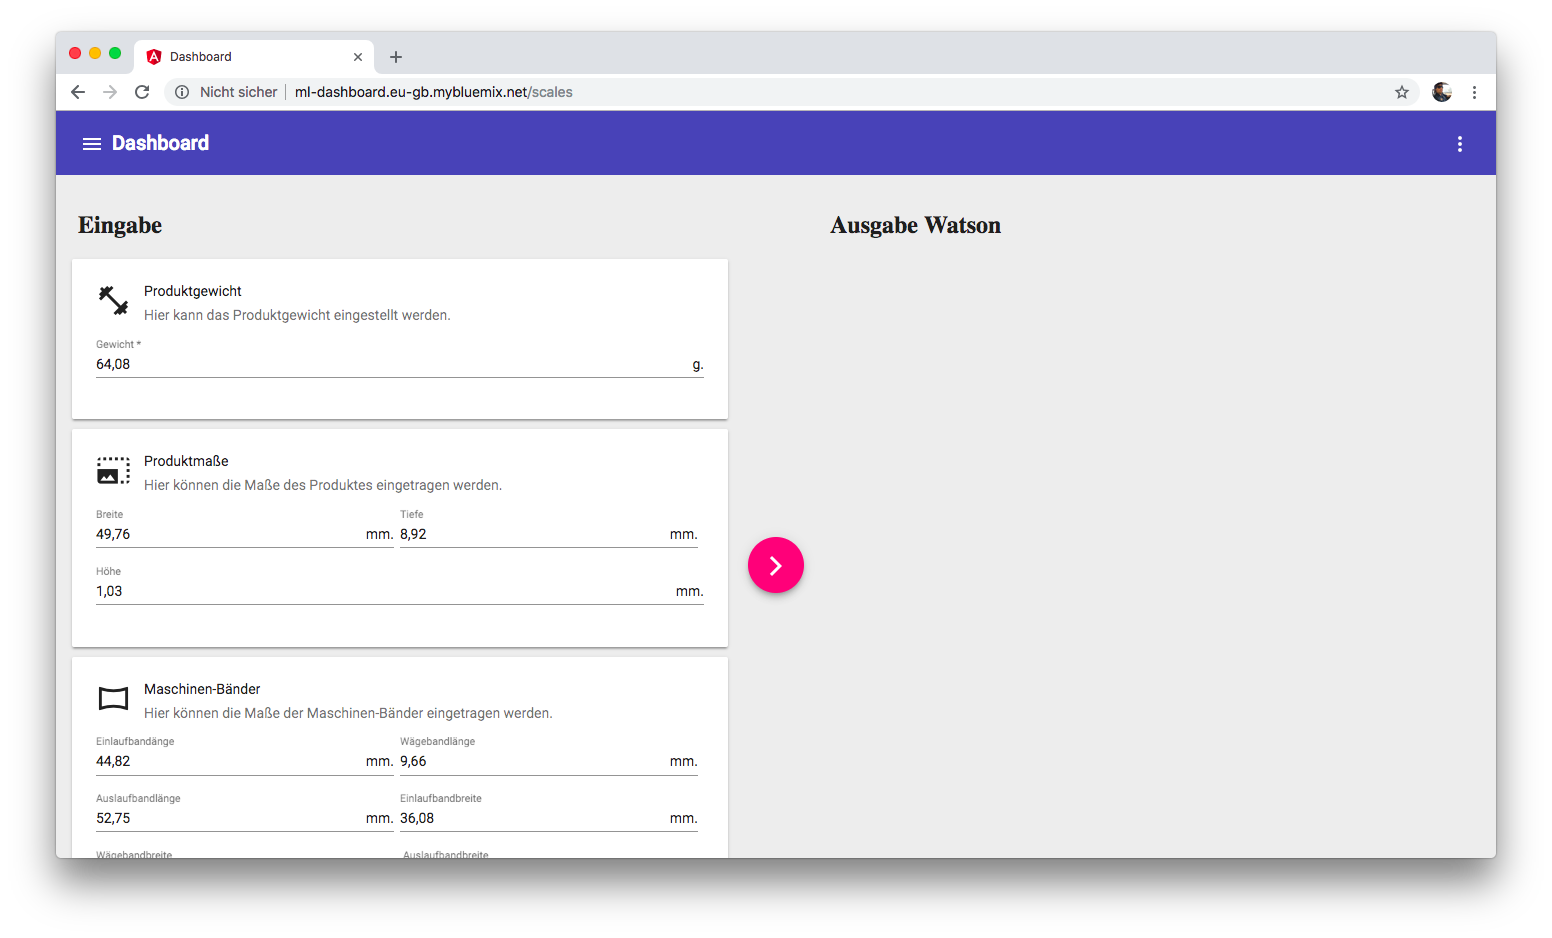
\includegraphics[width=\textwidth]{images/kapitel_4/website_input.png}
    \caption{Umsetzung der Webseite mit Eingabe-Spalte}
    \label{fig:umsetzung_website_input}
\end{figure}

Nun kann man die zweite Spalte mit der \textit{Ausgabe} anfertigen um sie in dem noch leeren Platz zu positionieren. Die
Umsetzung ist dabei gleich der Umsetzung mit der linken Spalte.

In der Abbildung~\ref{fig:umsetzung_website_output} auf Seite~\pageref{fig:umsetzung_website_output} ist die komplette
Webseite zu sehen mit beiden Spalten und dem Button zur generierung der Vorhersage.

\begin{figure}[h]
    \centering
    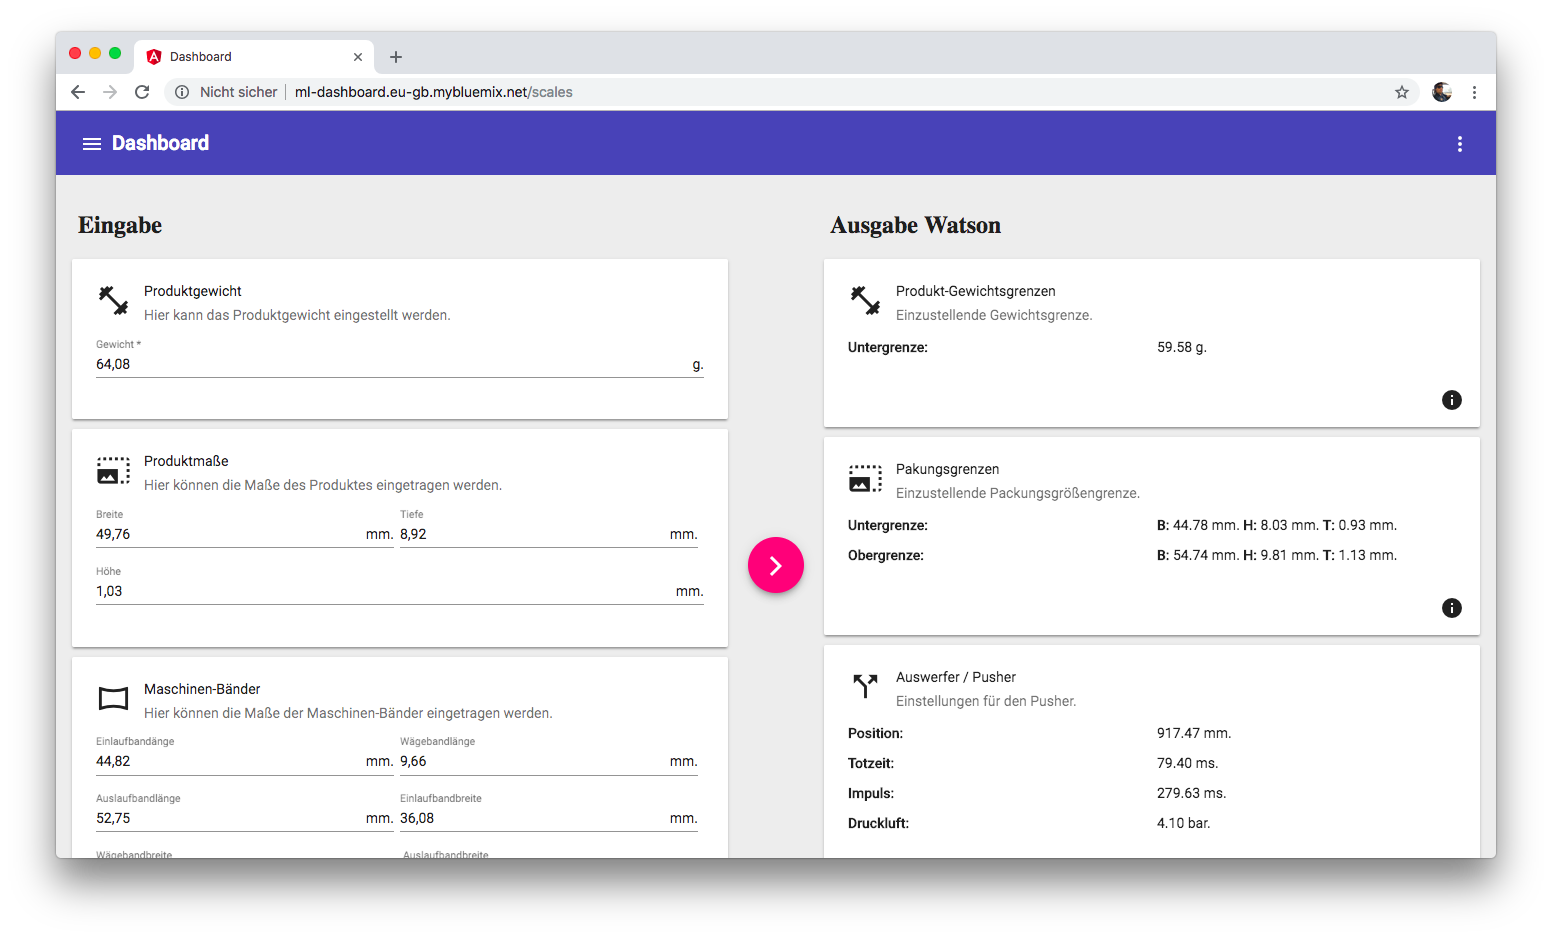
\includegraphics[width=\textwidth]{images/kapitel_4/website_output.png}
    \caption{Umsetzung der Webseite mit Ausgabe-Spalte}
    \label{fig:umsetzung_website_output}
\end{figure}

Bei der Umsetzung ist entscheidend, dass die rechte Spalte des Dashboards nur dann angezeigt wird, wenn auch die Abfrage
an das Backend durch ist und Vorhersagen an das Frontend zurück gekommen sind. Allerdings sollte man die Überschrift
der Spalte anzeigen -- Ausgabe -- damit der Endnutzer weiß, dass da noch weitere Informationen
folgen werden.

Auch ist so ersichtlich, dass der Platz auf der rechten Seite nicht verschwendet wird. Wenn die Eingabe der Parameter
sich über die gesamte Seite ziehen würde und nach betätigung des Buttons dann verkleinert, würde das zu viel bewegung in
der Webseite nach sich ziehen. Das wirkt sich negativ auf das verständnis der Webseite aus.

Die einzelnen Blöcke der Ausgabe erscheinen nach und nach durch kleine Animationen, welche die einzelnen Boxen langsam
einblendet. Dadurch kann man Zeit gewinnen, um das JSON-Objekt, welches vom Backend zurück kommt, zu parsen. Die einzelnen
Werte muss man sich aus dem großen Array herausziehen.

Das Parsen kann zeitgleich mit der Animation starten. So wird de Endnutzer symbolisiert, dass die Daten schon da sind
und sie auch gleich sichtbar sind. So muss er nicht noch das Parsing abwarten.

Dies erleichtert die Arbeit mit der Webseite enorm, da der Endnutzer nicht direkt mit vielen Boxen konfrontiert wird.
Außerdem existieren für die rechte Spalte nach dem öffnen der Seite auch noch keine Daten die angezeigt werden könnten.
So macht eine Darstellung des Bereiches auch keinen Sinn.

Damit der Endnutzer sich schneller auf der Webseite zurecht finden kann, ist die Platzierung von kleinen Icons und
Beschreibungstexten an den verschiedenen Boxen sinnvoll. So weiß der Nutzer direkt, was er in welcher Box machen oder
auch Einstellen kann.

Sinnvoll ist es auch die Parameter der linken Spalte mit passenden Zufallszahlen zu versehen. So kann der Nutzer direkt
nach dem öffnen der Seite eine Vorhersage starten um die Funktionsfähigkeit der Webseite und des Backends zu testen.
Auch kann er so nachvollziehen, welche Werte er in der linken Spalte eintragen muss, falls er sich zuanfang noch
unsicher ist.

Als nächsten Schritt muss man die Anpassung der Webseite an einen kleineren Bildschirm machen. Die Darstellung kann den
Mockups entnommen werden. Da die beiden Spalten (Eingabe und Ausgabe) in jeweils einer eigenen Angular-Komponente
entwickelt sind, kann man diese in eine \textit{CSS-FlexBox} packen.

Damit ist es möglich zu definieren, wie sich die einzelnen \textit{FelxBoxen} verhalten, wenn der Platz nicht
ausreichend ist. Dabei gibt man an, dass die Boxen sich im normalen Fall nebeneinander befinden. Falls dann der Platz
nicht ausreicht, sollen sie sich untereinander anordnen.

Dabei ist wichtig, dass der Button in der Mitte auch eine FlexBox erhält, damit dieser bei kleinem Platz auch
umgebrochen werden kann. Die Umbrechnung übernimmt die Bibliothek automatisch und es bedarf keiner weiteren
Konfiguration.

Ein Test mit einem mobilen Browser oder den Dev-Tools des Explorers \textit{Chrome} oder auch \textit{FireFox} zeigt die
Abbildung~\ref{fig:umsetzung_website_smartphone} auf Seite~\pageref{fig:umsetzung_website_smartphone}. Es ist lediglich
die \textit{Eingabe}-Spalte zu sehen.

\begin{figure}[h]
    \centering
    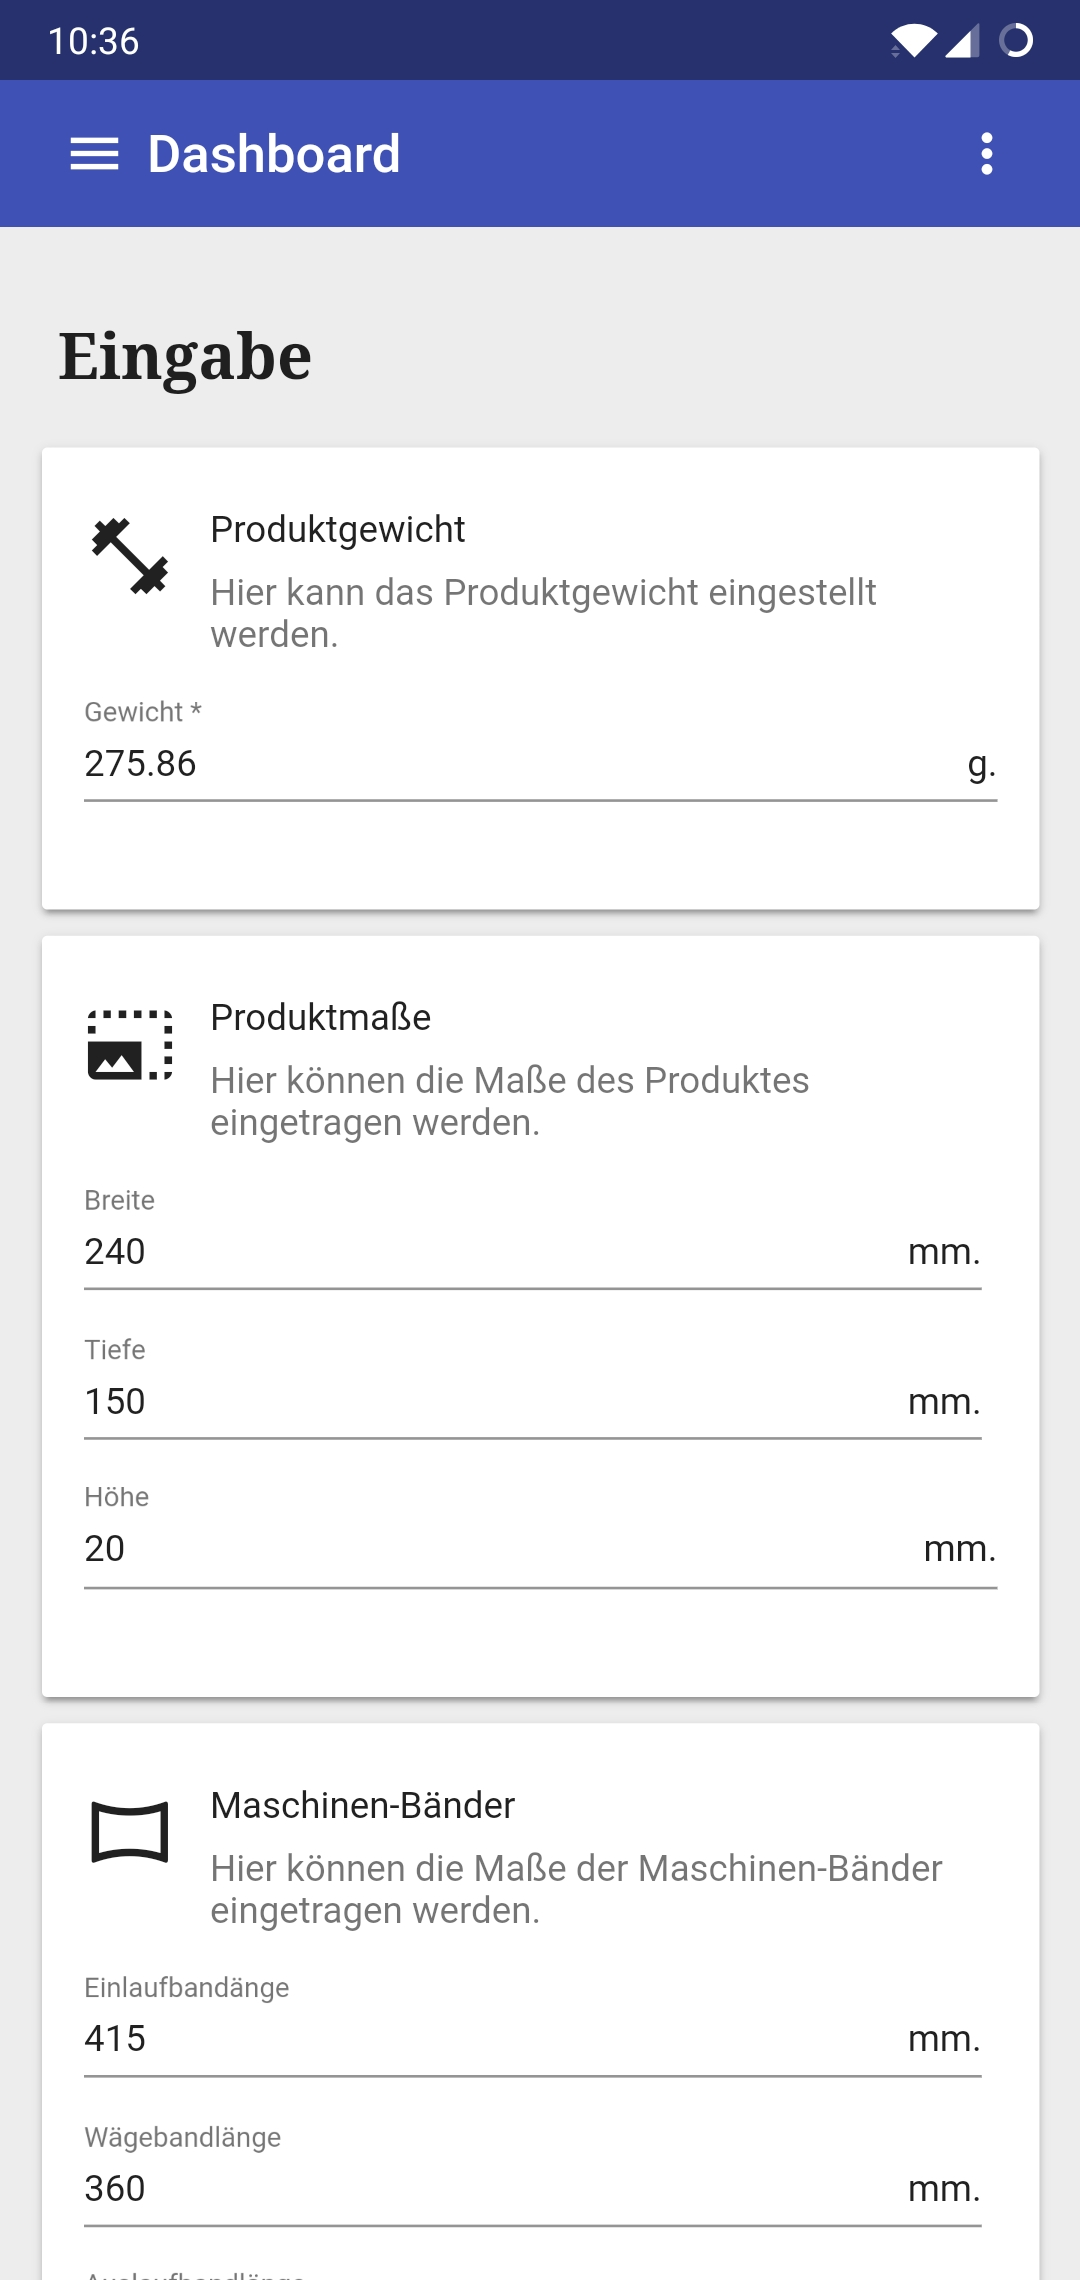
\includegraphics[scale=0.13]{images/kapitel_4/website_smartphone.jpg}
    \caption{Umsetzung der Webseite mit responiven Fähigkeiten}
    \label{fig:umsetzung_website_smartphone}
\end{figure}

Bei der Eingabe der einzlenen Formularfelder scrollt man unweigerlich nach unten. Am Ende der Eingabe erscheint dann der
Button zum erstellen der Vorhersage für die Parameter.

Nach einem Klick auf diesen Button und einer kurzen Ladeanimation erscheint die Ansicht der Ausgabe. Der Nutzer muss
nicht mehr nach unten scrollen.

Auch in der mobilen Version steht die Überschrift für die Ausgabe schon am unteren Rand, damit der Endnutzer weiß, dass
die Informationen unterhalb der Eingabe kommen werden und er nicht unnötig überrascht wird.

\subsubsection{Erweiterungen}
Die Webseite ist fertig entwickelt. Nun kann man sich über Erweiterungen Gedanken machen, die den Endnutzer bei der
Eingabe der Daten unterstützen können.

Für zahlreiche Erweiterungen, welche im folgenden Behandelt werden, spielt der \textit{Service Worker} eine
entscheidende Rolle. Dieser installiert, definiert über ein Manifest, mittels JavaScript-Technologie einen Proxy
zwischen dem Webbrowser und dem Server.

Damit kann man die Grundlage für Push-Benachrichtigungen, progressive Web-Apps (PWA), offline Modus und komplexer
Cache-Strategie setzen.

Um in der erstellten Angular-Anwendung einen Service-Worker zu installieren, benötigt man eine zusätzliche Bibliothek,
welche die interne Arbeit übernimmt. Diese kann man mittels des folgenden Befehls in die Anwendung einbauen.

\begin{lstlisting}[language=bash, caption=Hinzufügen der PWA-Bibliothek, label=ls:umsetzung_angularaddpwa]
    ng add @angular/pwa
\end{lstlisting}

Nun muss man den ServiceWorker in der \textit{angular.json}-Datei aktivieren. Dazu fügt man die Zeile
\textit{"serviceWorker": true} in das erste \textit{apps}-Objekt ein.

Mit der Aktivierung der Funktionalität wird beim Bau der Anwendung eine \textit{Angular Service Worker}-Datei mit dem
Namen \textit{ngsw-worker.js} angelegt. Außerdem wird eine Konfigurationsdatei für den Service Worker mit dem Namen
\textit{ngsw.json} angelegt.

Die erste Datei übernimmt die Installation, das Aktualisieren und das Deinstallieren des Service Workers in den Browser.
Die zweite Datei kann den Service Worker konfigurieren. So kann man dort zum Beispiel definieren, wie der Service Worker
heißt und welches Icon für ihn angezeigt werden soll.

Die Einrichtung des Service Workers ist damit abgeschlossen. Allerdings funktioniert dieser nur, wenn die
Angular-Anwendung produktiv gebaut wird (\textit{ng build --prod}) und dann über das Protokoll \textit{https} aufgerufen
wird.

Wenn man im Nachgang die Webseite aufruft (mehr dazu im Kapitel~\ref{toolchain_einrichten} auf
Seite~\pageref{toolchain_einrichten}), kann man den Service Worker in den \textit{Entwicklertools} über den Menüpunkt
\texttt{Applikation} und dann \texttt{Service Worker} sehen. Dort kann man ihn auch zur Aktualisierung zwingen und
Löschen.

\subsubsection{Offline Modus}
Da man im vorangegangenen Kapitel den Service Worker installiert und eingerichtet hat, kann man als nächstes eine der
grundlegensten Funktionen des Service Workers nutzen -- das Caching mit offline Modus.

Damit man diesen umsetzen kann, muss man lediglich die Datei \textit{ngsw.json} anpassen und um alle cachbaren Elemente
erweitern.

In Anhang~\ref{sec:serviceWorkerConfig} auf Seite~\pageref{sec:serviceWorkerConfig} ist die komplette
Konfigurationsdatei angegeben. Diese kann man komplett nutzen. Nachdem man die Angular-Anwendung wieder gebaut hat, kann
man sie aufrufen und alle Elemente werden automatisch im Browser gecached.

Wenn man im Anschluss die Internetverbindung unterbricht (offline Modus oder Netzwerk trennen) und die Webseite
aktualisiert, wird sie trotzdem wie gewünscht angezeigt. Allerdings kann man in diesem Fall keine Vorhersagen tätigen,
da die REST-Schnittstelle nicht aufgerufen werden kann.

Der offline Modus funktioniert auf allen Plattformen in allen Browsern. So kann man diesen sowohl auf dem Desktop-Computer
nutzen als auch auf dem Smartphone oder Tablet.

\subsubsection{Keine offline Abfragen}
Damit man im offline Modus nicht auf einen Fehler stößt, wenn man eine Abfrage an das Backend machen möchte, soll im
Weiteren das Frontend auf die verschiedenen Modi (online oder offline) reagieren können.

Beispielhaft soll man sich folgendes Szenario vor Augen führen. Ein Endnutzer öffnet bei aktiver Internetverbindung die
Webseite um eine Vorhersage zu tätigen. Damit er die geforderten Eingabeparameter allerdings eingeben kann, muss er zur
betreffenden Maschine und diese auslesen.

In dem Raum in dem sich die Maschine befindet gibt es allerdings keine WLAN Verbindung, worauf die Webseite in den
offline Modus geht. Nachdem der Endnutzer die Daten eingetragen hat und eine Vorhersage starten will, würde er einfach
eine Fehlermeldung bekommen, dass das Backend nicht angefragt werden kann. Eventuell würden seine Eingaben auch
verschwinden, da er versucht die Seite neu zu laden.

Um dieses Problem zu beheben, soll das Frontent im offline Modus gar keine Anfragen an das Backend machen sondern den
Nutzer informieren, dass es aktuell im offline Modus ist. Damit weiß der Nutzer, dass er aktiv nach einer
Internetverbindung suchen muss.

Um dies zu bewerkstelligen muss man einen Service in die Angular-Anwendung einbauen, welcher immer über den aktuellen
Modus (online oder offline) bescheid weiß und bei einer Änderung allen Komponenten bescheid gibt.

Mit dem folgenden Befehl kann man einen neuen Service in die Anwendung einbauen.

\begin{lstlisting}[language=bash, caption=Hinzufügen eines Services, label=ls:umsetzung_angularaddservice]
    ng generate service network
\end{lstlisting}

Dieser Befehl legt eine Datei mit dem Namen \textit{network.service.ts} an, in der der Service definiert wird. Die
Implementierung der geforderten Funktion ist relativ einfach, da Angular von Haus aus viele Funktionalitäten mitbringt.

So kann man mit dem in Listing~\ref{ls:umsetzung_angularservicenetwork} auf
Seite~\pageref{ls:umsetzung_angularservicenetwork} definierten Quellcode ein \textit{Observable} anlegen, welches den
aktuellen Netzwerkmodus beinhaltet. Sollte dieser sich ändern, werden alle \textit{Observer} darüber informiert.

\begin{lstlisting}[language=JavaScript, caption=Funktion des Network-Services, label=ls:umsetzung_angularservicenetwork]
    public isConnected = true;

    constructor(private connectionService: ConnectionService) {
        this.connectionService.monitor().subscribe(isConnected => {
            this.isConnected = isConnected;
        })
    }
\end{lstlisting}

Die vierte Zeile \textit{subscribed} sich auf einen Angular internen \textit{Observable}, welcher die Information
beinhaltet, ob eine Internetverbindung aktuell besteht oder nicht. Die Information, welche aus dem internen Service
kommt, wird in der lokalen Variable \textit{isConnected} gespeichert. Diese Speicherung führt man in Zeile fünf durch.

Die Varibale, die den aktuellen Modus der Internetverbindung hält, definiert man am Besten global in dem Service und
damit weit oben in der Datei. Hier symbolisiert durch die Zeile eins.

Anschließend kann man bei jeder Anfrage an das Backend das in Listing~\ref{ls:umsetzung_angularchecknetwork} auf
Seite~\pageref{ls:umsetzung_angularchecknetwork} definierte If-Statement nutzen, um zu überprüfen ob aktuell eine
Internetverbindung vorliegt oder nicht. Falls nicht, sollte man den Nutzer über einen gut sichtbaren Hinweis darüber
informieren, dass aktuell keine Abfrage möglich ist.

\begin{lstlisting}[language=JavaScript, caption=Überprüfung ob eine Internetverbindung vorliegt, label=ls:umsetzung_angularchecknetwork]
    if (this.networkService.isConnected) {
        ...
    } else {
        ...
    }
\end{lstlisting}

In der Zeile zwei definiert man den Programmteil, welcher bei aktiver Internetverbindung aufgefürt wird. Also zum
Beispiel die Abfrage an das Backend. In der vierten Zeile kann man dann die Meldung ausgeben die angezeigt wird, wenn
der Nutzer über keine Internetverbindung verfügt.

Auch wäre es möglich einen dauerhaften Hinweis einzublenden, wenn keine Internetverbindung vorliegt. Dies müsste man dann
in der \textit{app.component.ts} Datei global machen. Dabei ist entscheidend, dass das nicht mit einem If-Statement
möglich ist.

Mit einer Snackbar kann man den entsprechenden Hinweis optimal anzeigen und positionieren lassen.

\subsubsection{Toolchain einrichten}
Im letzten Schritt bei der Entwicklung des Frontends muss man die Toolchain einrichten, damit man den geschriebenen
Quellcode auch in einem Cloud Foundry Container in der Cloud installieren kann.

Dabei ist die Konfiguration der Pipeline nicht ganz so einfach wie die beim Erstellen des TensorFlow-Containers, da man
die Angular-Anwendung bauen muss, bevor man sie in den Container schieben kann. Auch ist der gebaute Quellcode in einem
anderen Ordner als der Teil, welchen man in das Git-Repository lädt. So sind nacheinander wenige Schritte notwendig,
damit man die gebaute Anwendung auch richtig in den Container schieben kann.

In einem ersten Schritt muss man die Toolchain jedoch erst anlegen. Dies kann man über das Cloud Foundry Dashboard der
IBM Cloud machen. Dazu geht man auf das IBM Cloud Dashboard und Klickt auf die angelegte Runtime der Angular-Anwendung.

Nun öffnet sich das Cloud Foundry Dashboard über das man am unteren Bereich auf den Button \texttt{Aktivieren} in der
Box \texttt{Continous Delivery} Klicken kann. Genau wie in Kapitel~\ref{sub:tollchain_einrichten} auf
Seite~\pageref{sub:tollchain_einrichten} gelangt man damit auf die Konfigurationsseite der Toolchain.

Nun muss man einen Namen für die Toolchain definieren und die Region auswählen. Da auch hier die Standartkonfiguration
ausreicht, kann man die Toolchain mit einem Klick auf den Button \texttt{Erstellen} einrichten.

Nach einem kurzen Ladevorgang ist die Toolchain eingerichtet und mit einem leeren Git-Repository vorkonfiguriert.
Aktuell ist lediglich die \textit{Delivery Pipeline} interessant, da man hier die Installation der Angular-Anwendung
spezifizieren muss.

In der aktuellen Konfiguration sind drei \textit{Stages} eingerichtet. Diese muss man nun um zwei weitere Ergänzen,
sodass es eine \textit{Build-}, eine \textit{Angular build-}, eine \textit{Copy files-}, eine \textit{Test} und eine
\textit{Deploy}-Stage gibt. Dies ist in Abbilung~\ref{fig:umsetzung_toolchain_pipeline_frontend} auf
Seite~\pageref{fig:umsetzung_toolchain_pipeline_frontend} ersichtlich.

\begin{figure}[h]
    \centering
    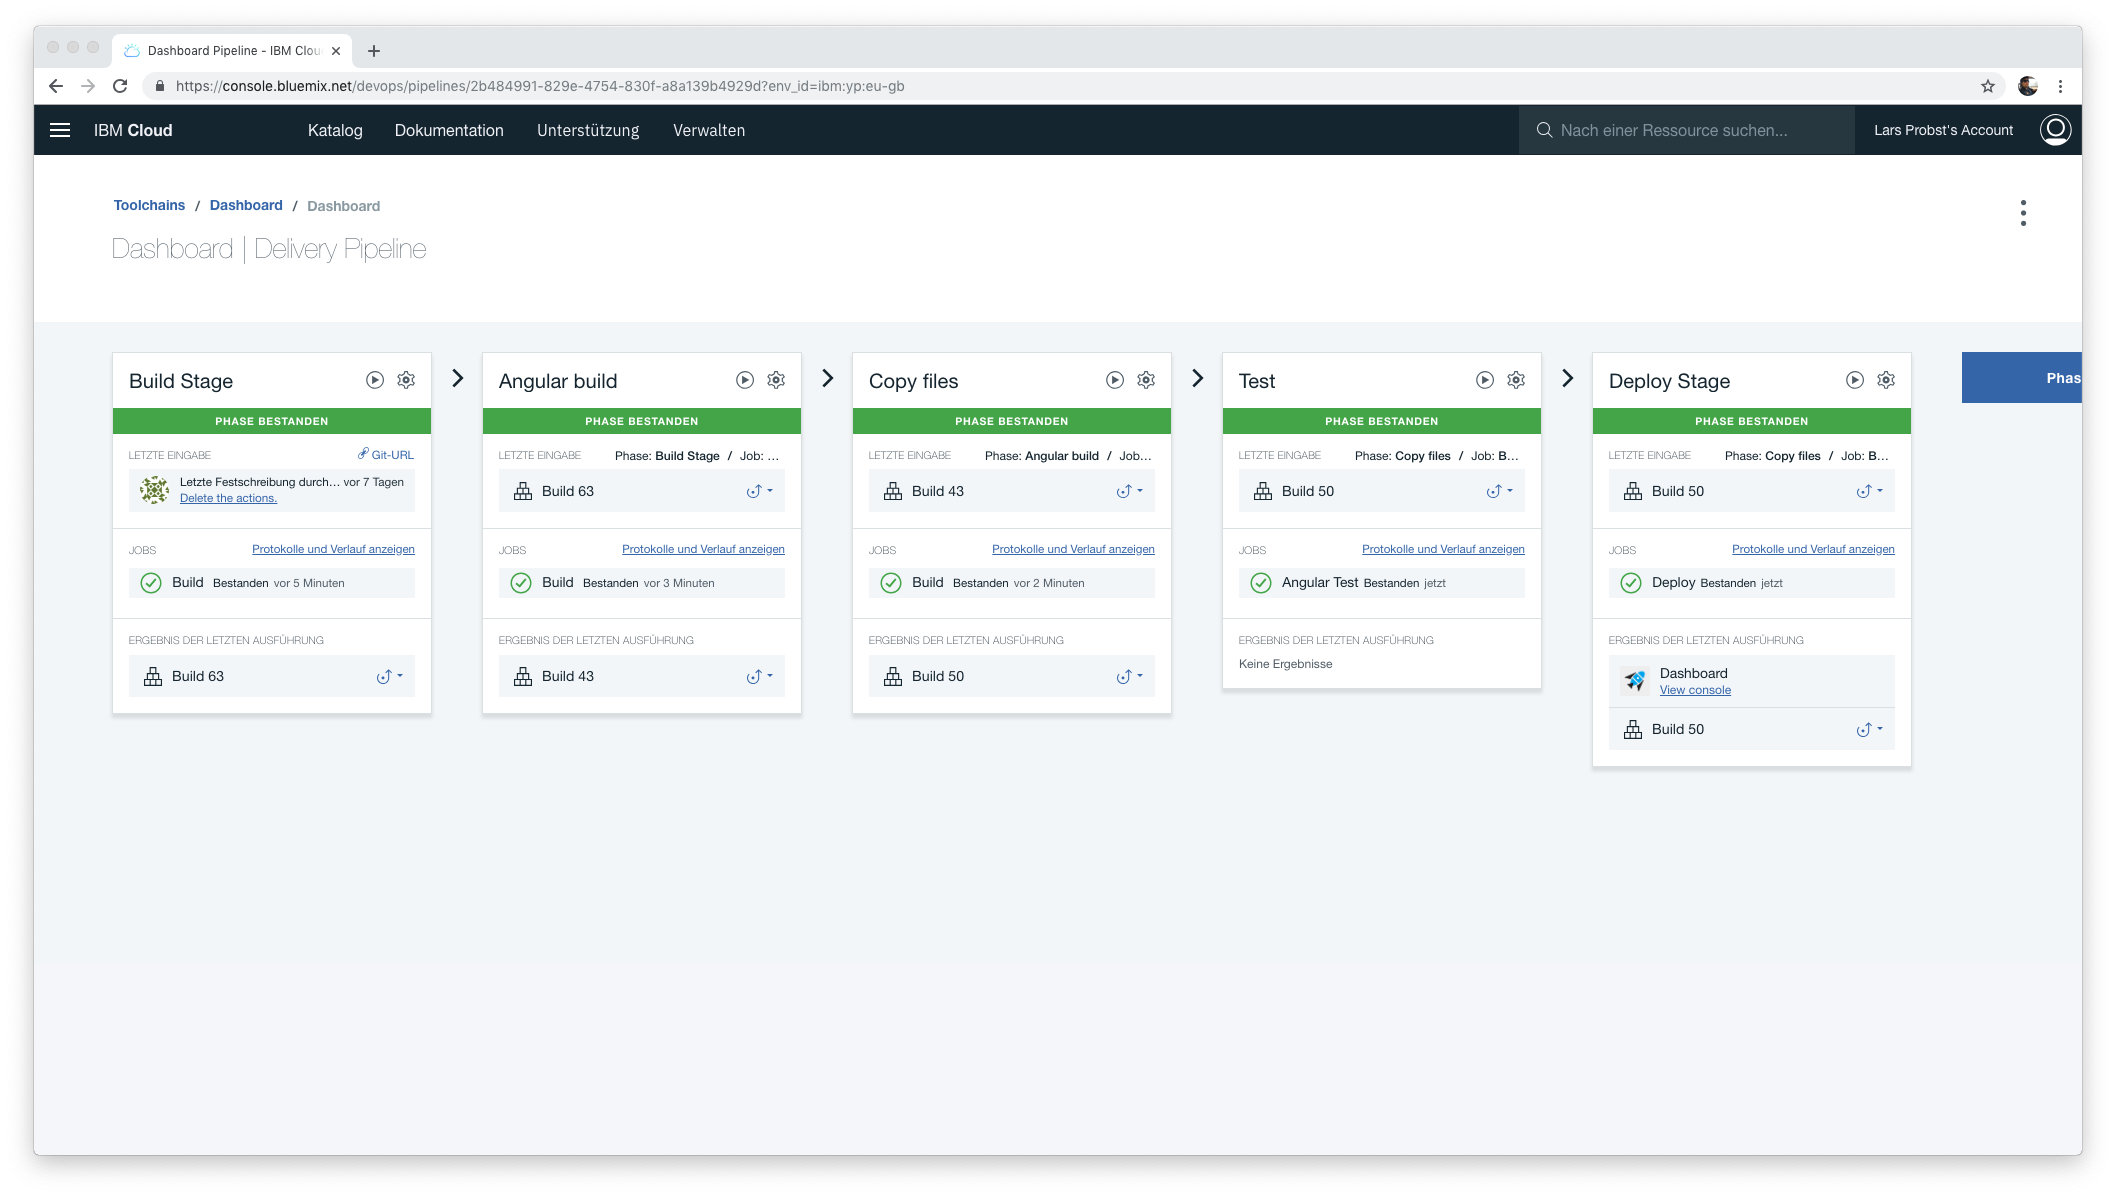
\includegraphics[width=\textwidth]{images/kapitel_4/toolchain_pipeline.png}
    \caption{Übersicht der Toolchain-Konfiguration}
    \label{fig:umsetzung_toolchain_pipeline_frontend}
\end{figure}

Die \textbf{Build Stage} entspricht der Standard Build Stage der Toolchain konfiguration und man kann diese unverändert
beibehalten. Sie ist für das Laden des Quellcodes aus dem Git-Repository zuständig und wird immer dann ausgeführt,
sobald ein \textit{commit} in das Repository \textit{gepushed} wird.

In der \textbf{Angular Build} Stage wird die ANgular-Anwendung mittels des Befehls \textit{ng build --prod} gebaut. Dies
ist wichtig, damit ein \textit{dist}-Ordner entsteht, welcher alle kaskadierten CSS- und HTML-Dateien enthält. Auch
werden CSS- oder HTML-Platzhalter ausgetauscht und die Angular-Anwendung betriebsbereit geschaltet. Dies ist zum
Beispiel auch für den offline Modus und den Service Worker entscheidend.

Die nächste Stage, \textbf{Copy files}, kümmert sich um das Kopieren der Inhalte aus dem \textit{dist}-Ordner. Später
soll in dem Cloud Foundry Container nicht der Quellcode laufen, welcher in das Git-Repository geladen wurde. Sondern
der, welcher mittels der vorangegangenen Stage durch die Angular-CLI gebaut wurde. Darum muss man, bis auf den Inhalt
des dist-Ordners, alle Dateien und Ordner löschen.

Um die Funktionalität einer Anwendung stetig gewährleisten zu können sollte man Tests für alle Funktionen bereitstellen.
Die \textbf{Test}-Stage kümmert sich um die Ausführung der Tests. Nur wenn alle erfolgreich durchlaufen, wird der Inhalt
an das Deployment übergeben um den Cloud Foundry Container zu befüllen.

Die letzte Stage, \textbf{Deploy Stage}, ist die Stadard-Stage der Toolchain für das Installieren der Anwendung. Diese
kann aus der Ursprungskonfiguration übernommen werden.

Somit ist die Toolchain fertig konfiguriert und man kann den Quellcode in das Git-Repository laden um die Toolchain zu
starten. Nach wenigen Minuten ist die Anwendung in einem Cloud Foundry Container über ihre Domain im Browser aufrufbar
und man kann damit beginnen Anfragen an das Backend zu stellen.

Da man in Kapitel~\ref{subsec:apiconnect} auf Seite~\pageref{subsec:apiconnect} den API Connect Service mit den beiden
Backends verbunden hat, kann man nun aus dem Frontend heraus Anfragen an diese stellen und die Vorhergesagten Parameter
werden angezeigt.

Im Weiteren kann man damit beginnen das Frontend in die Smartphone-Apps einbauen, da es über eine Domain und ein
valides SSL-Zertifikat verfügt.

Nur damit ist es Möglich die Webseite in ein WebViewer zu laden und dem Endnutzer anzuzeigen. Auch für die
Funktion des Service Workers und des offline Moduses ist ein SSL-Zertifikat und eine Domain essentiell.

\subsection{Smartphone App}
Da das Frontend (Dashboard) nun fertig entwickelt ist, kann man es im nächsten Schritt für die Umsetzung der
Smartphone-App nutzen.

Die Umsetzung der Smartphone-App erfolgt auf Basis von Android und iOS. Dies hat den Vorteil, dass ein größerer
potentieller Kundenkreis gewonnen werden kann, da diese beiden Systeme die mobilen Betriebssysteme
dominieren~\cite{online_umsetzung_mobileos}.

In den zwei weiteren Kapiteln werden die Umsetzungen für die beiden Betriebssysteme erläutert. Insbesondere wird auf die
technischen Unterschiede der Systeme eingegangen.

\subsubsection{Android}
Für die Erstellung einer Android-App benötigt man die Android Studio IDE. Diese kann man kostenlos auf der
Developper-Seite\footnote{https://developer.android.com/studio} von Google herunterladen. Die Anwendung steht für
Windows, Linux und macOS zur Verfügung. Android Studio basiert auf der Community-Edition von IntelliJ1.

Für die Verwendung von Android Studio benötigt man eine Installierte Java-JRE und das Java-JDK. Die JRE benötigt man für
das Ausführen der IDE und die JDK für das Bauen des Qqellcodes und der APK-Datei. Die Aktuellste Version von Java wird
für die Nutzung empfholen. Dies ist zur Zeit die Version 9.

Nachdem man die IDE und gegebenenfalls Java installiert hat, kann man Android Studio zum ersten Mal starten. Beim ersten
Aufruf muss man das Android-SDK herunterladen sowie einen Emulator konfigurieren. Dabei sollte man jeweils die neuesten
Versionen auswählen. Mit dem Emulator kann man die App nachher auf dem Rechner starten und live testen.

Im nächsten Schritt muss man ein neues Projekt anlegen. Dazu wird zum Beispiel der Name \textit{Dashboard} ausgewählt.
Also Projekttyp kann man ein leeres Android-Projekt auswählen. Dadurch werden keine Klassen oder Layouts angelegt.

Die Android-App muss im Ordner \texttt{/res/layout} ein Layout besitzen, welches als Root-Element ein
\textit{CoordinatorLayout} besitzt und als Kind-Element ein WebView Layout. Diesem Layout wird eine ID zugeteilt, damit
man es aus der Kotlin-Klasse heraus eindeutig identifizieren kann.

Nun kann man im \texttt{/src}-Ordner zwei Kotlin-Klassen anlegen. Eine für die MainActivity, welche die Hauptroutine der
Anwendung enthält. Die andere ist für den SplashScreen, welcher beim Start der App angezeigt wird. Der Splashscreen
zeigt das Bosch-Logo und wechselt nach ein paar Sekunden in die Hauptroutine um den WebViewer darzustellen.

Die MainActivity entählt eine unveränderliche Variable vom Typ \textit{Text} um die URL des Frontends zu definieren. In
der \textit{onCreate}-Methode kann man dann das WebViewer-Layout konfigurieren, damit die Nutzung von JavaScript möglich
ist.

Das WebView-Layout, welches von der \textit{Android-WebKit} Klasse erbt, kümmert sich anschließend um das Laden der
Webseite, die Darstellung und die Interaktion des Nutzers damit.

Wenn man Funktionen der \textit{WebViewClient} überschreibt kann man das Verhalten des WebViews anpassen. So kann man
beispielsweise Einfluss auf den Titel oder andere HTML-Elemente nehmen.

In den beiden Ordnern \texttt{/res/values} und \texttt{/res/values-v21} kann man Farben und Styles definieren. Im Ordner
mit der Endung \textit{v21} kann man Styles und Farben definieren, welche erst ab der Android in der Version 21 genutzt
werden.

Die Datei- und Ordnerstruktur der Android-Anwendung kann man in der Abbildung~\ref{fig:umsetzung_android_folder} auf
Seite~\pageref{fig:umsetzung_android_folder} einsehen.

\begin{figure}[h]
    \centering
    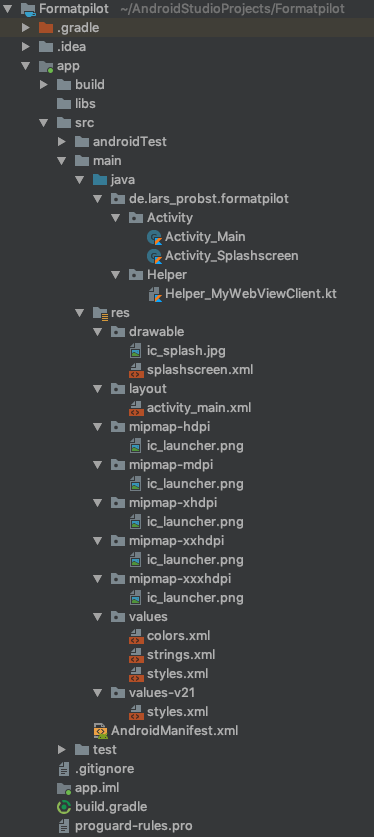
\includegraphics[scale=0.3]{images/kapitel_4/android_folder.png}
    \caption{Ordner und Dateien in Android Studio}
    \label{fig:umsetzung_android_folder}
\end{figure}

Der Ordner \texttt{/res/drawable} enthält das Splashscreen-Logo, also das Bosch-Logo, und die Konfiguration für den
Hintergrund des Splashscreens.

Die \textit{Manifest.xml}-Datei ist Elementar für jede Android-Anwendung. Über diese kann man die Informationen und
Konfigurationen der gesamten App anpassen.

Zum Beispiel ist es dort möglich zu definieren, welche Activity beim Start der Anwendung geladen werden soll. Weitere
Informationen zu dieser Manifest Datei sind in der
Android-Developer-Seite\footnote{https://developer.android.com/guide/topics/manifest/manifest-intro} verfügbar.

In der Abbildung~\ref{fig:umsetzung_android_app} auf Seite~\pageref{fig:umsetzung_android_app} ist die fertig
entwickelte Android-App in einem Smartphone-Emulator sichtbar.

\begin{figure}[h]
    \centering
    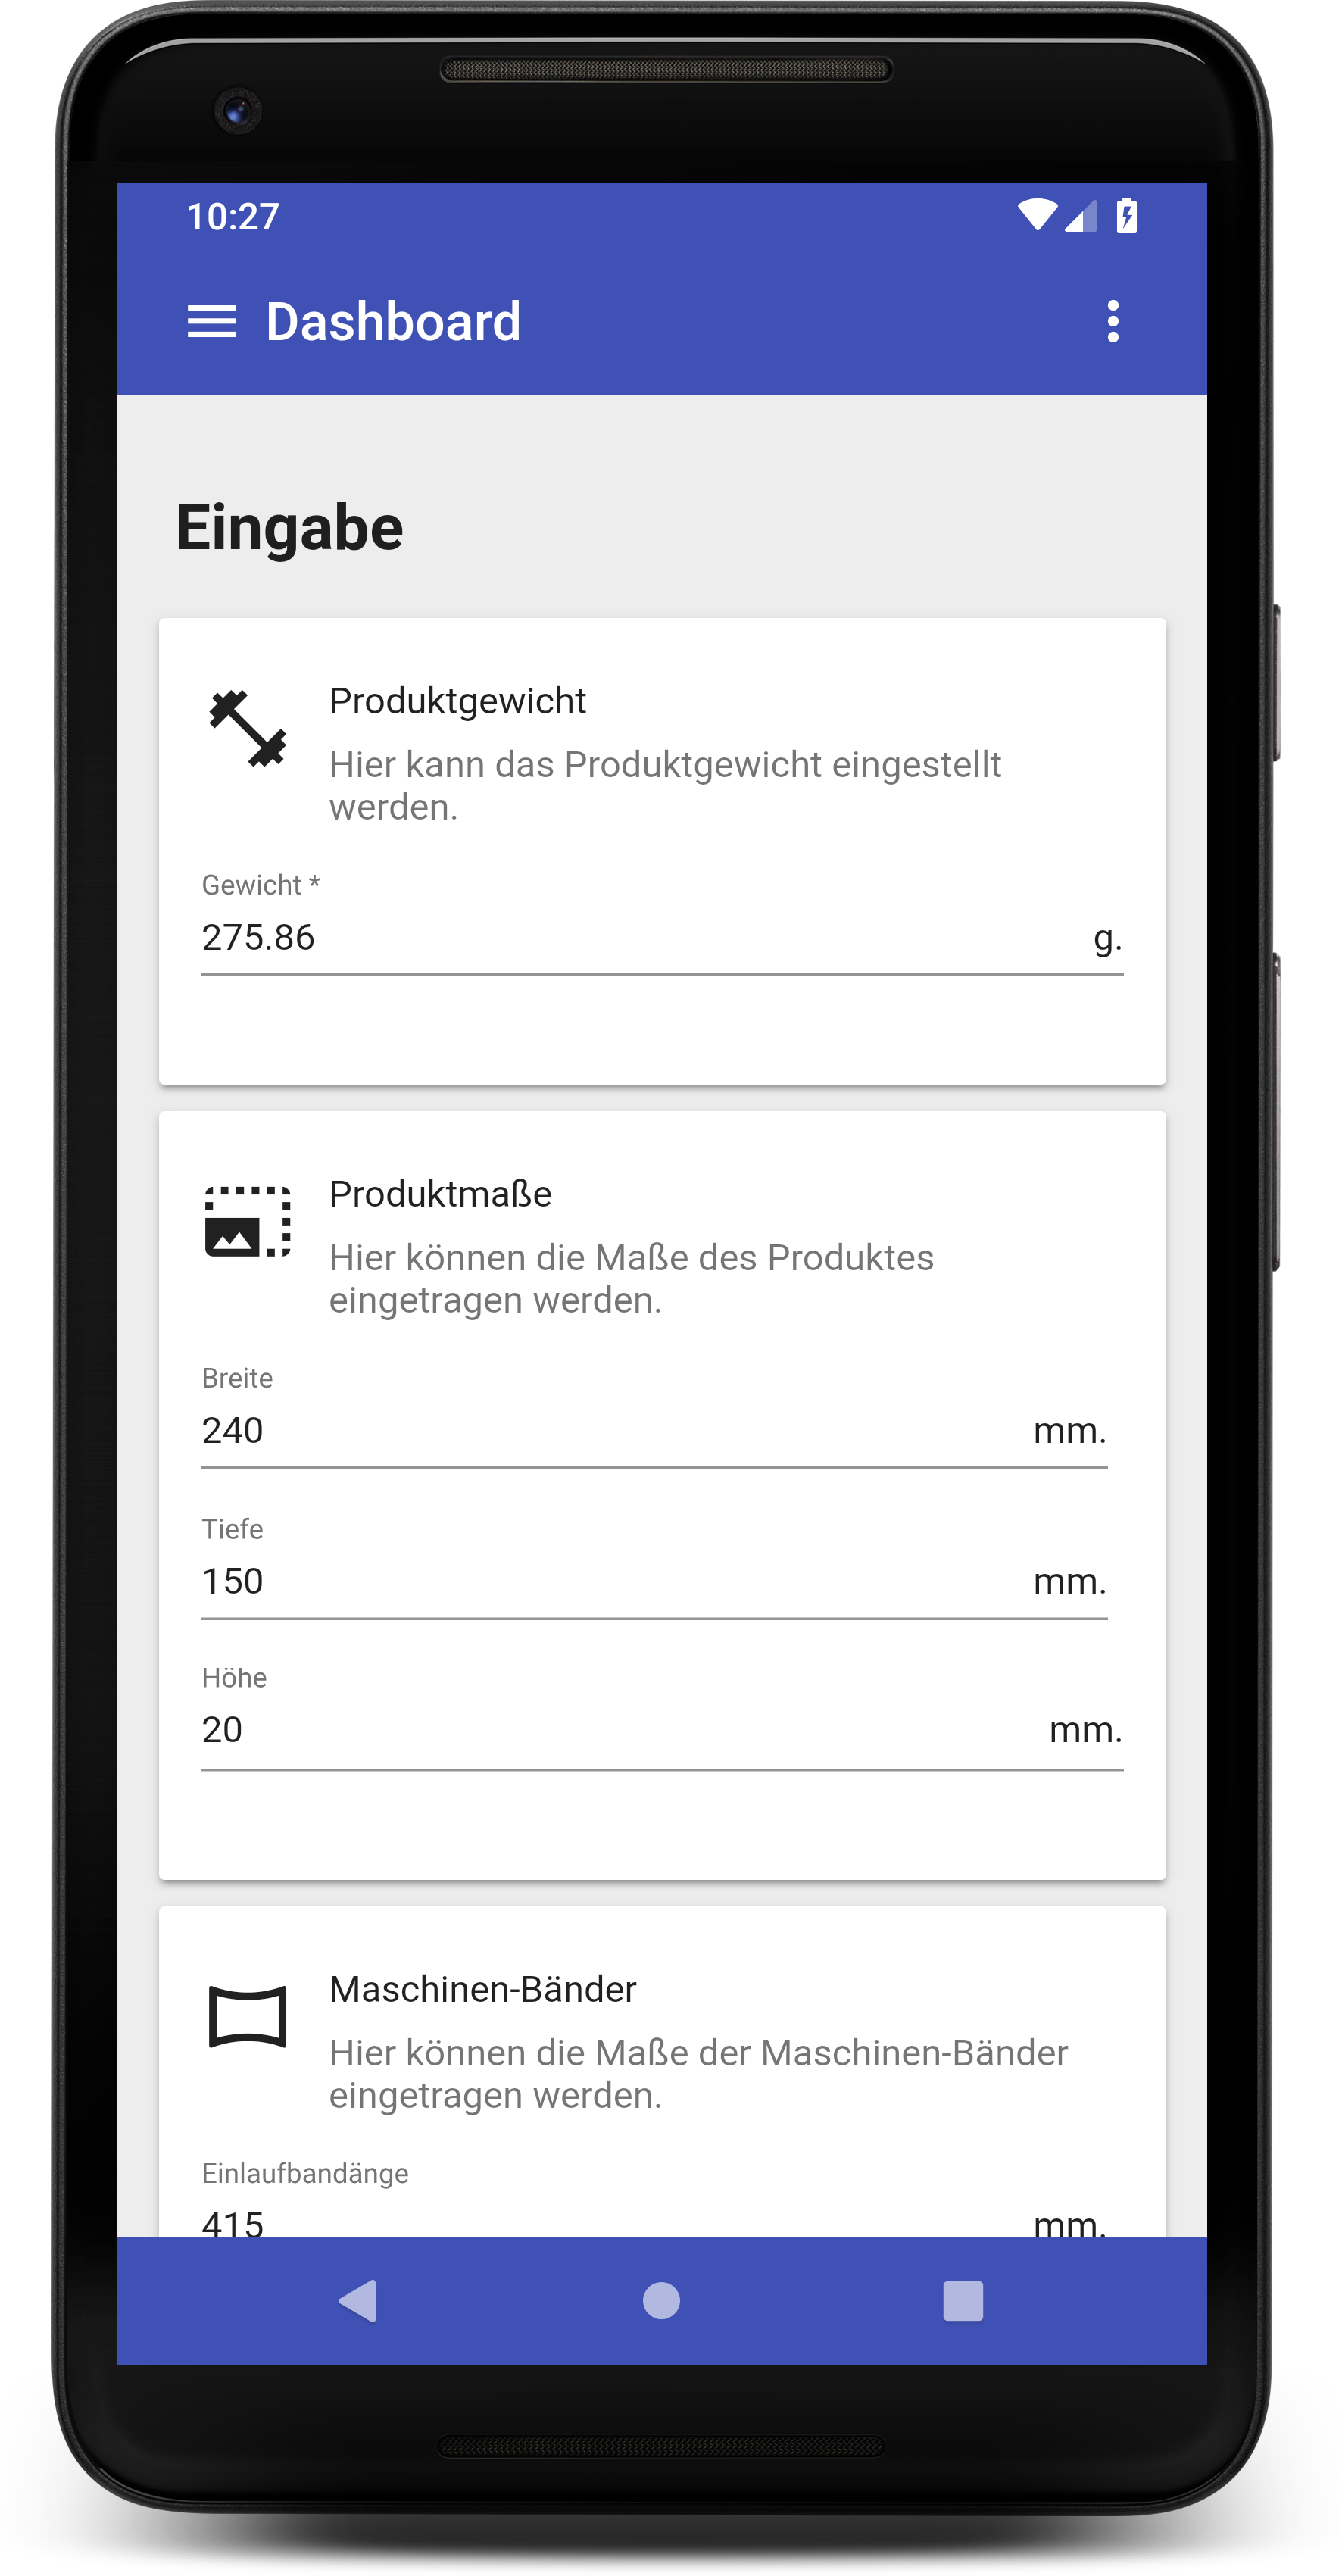
\includegraphics[scale=0.095]{images/kapitel_4/android_app.png}
    \caption{Android-App im Smartphone-Emulator}
    \label{fig:umsetzung_android_app}
\end{figure}

In dieser Abbildung ist leicht zu sehen, dass die Antroid-Styles direkten Einfluss auf die Darstellung der Menüpunkte
(am unteren Rand) und die Farbe der Toolbar haben. Beide werden in der selben Farbe wie der Header im Web-Frontend
dargestellt.

Die Android-App ist an dieser Stelle fertig entwickelt und man kann sie in eine APK-Datei exportieren. Dazu muss man
eine \textit{Signing-Datei} erstellen mit welcher es dann möglich ist, die Anwendung auch in den Play-Store zu laden.

Alternativ kann man die exportierte Android Package-Datei (kurz APK) auch auf einem echten Smartphone oder Tablet
installieren um sie unter echten Bedingungen zu testen.

\subsubsection{iOS}
Um eine App für iOS Geräte zu entwickeln, benötigt man die kostenlose IDE xCode von Apple. Diese steht lediglich für
macOS-Geräte zur Verfügung und man kann sie im App-Store\footnote{https://itunes.apple.com/de/app/xcode/id497799835?mt=12}
herunterladen.

Somit kann man iOS Apps lediglich unter macOS und xCode schreiben, kompilieren und testen. Dies stellt eine sehr große
Einschränkung dar.

Nach der erfolgreichen Installation kann man in xCode anschließend ein neues Projekt anlegen. Die Art des Projektes ist
\textit{SingleViewApp} und den Namen kann auf \textit{Dashboard} setzen.

In der Abbildung~\ref{fig:umsetzung_ios_ide} auf Seite~\pageref{fig:umsetzung_ios_ide} ist das erstellte Projekt in
xCode zu sehen. Der lokale Emulator und die verschiedenen SDKs sind automatisch mitinstalliert.

\begin{figure}[h]
    \centering
    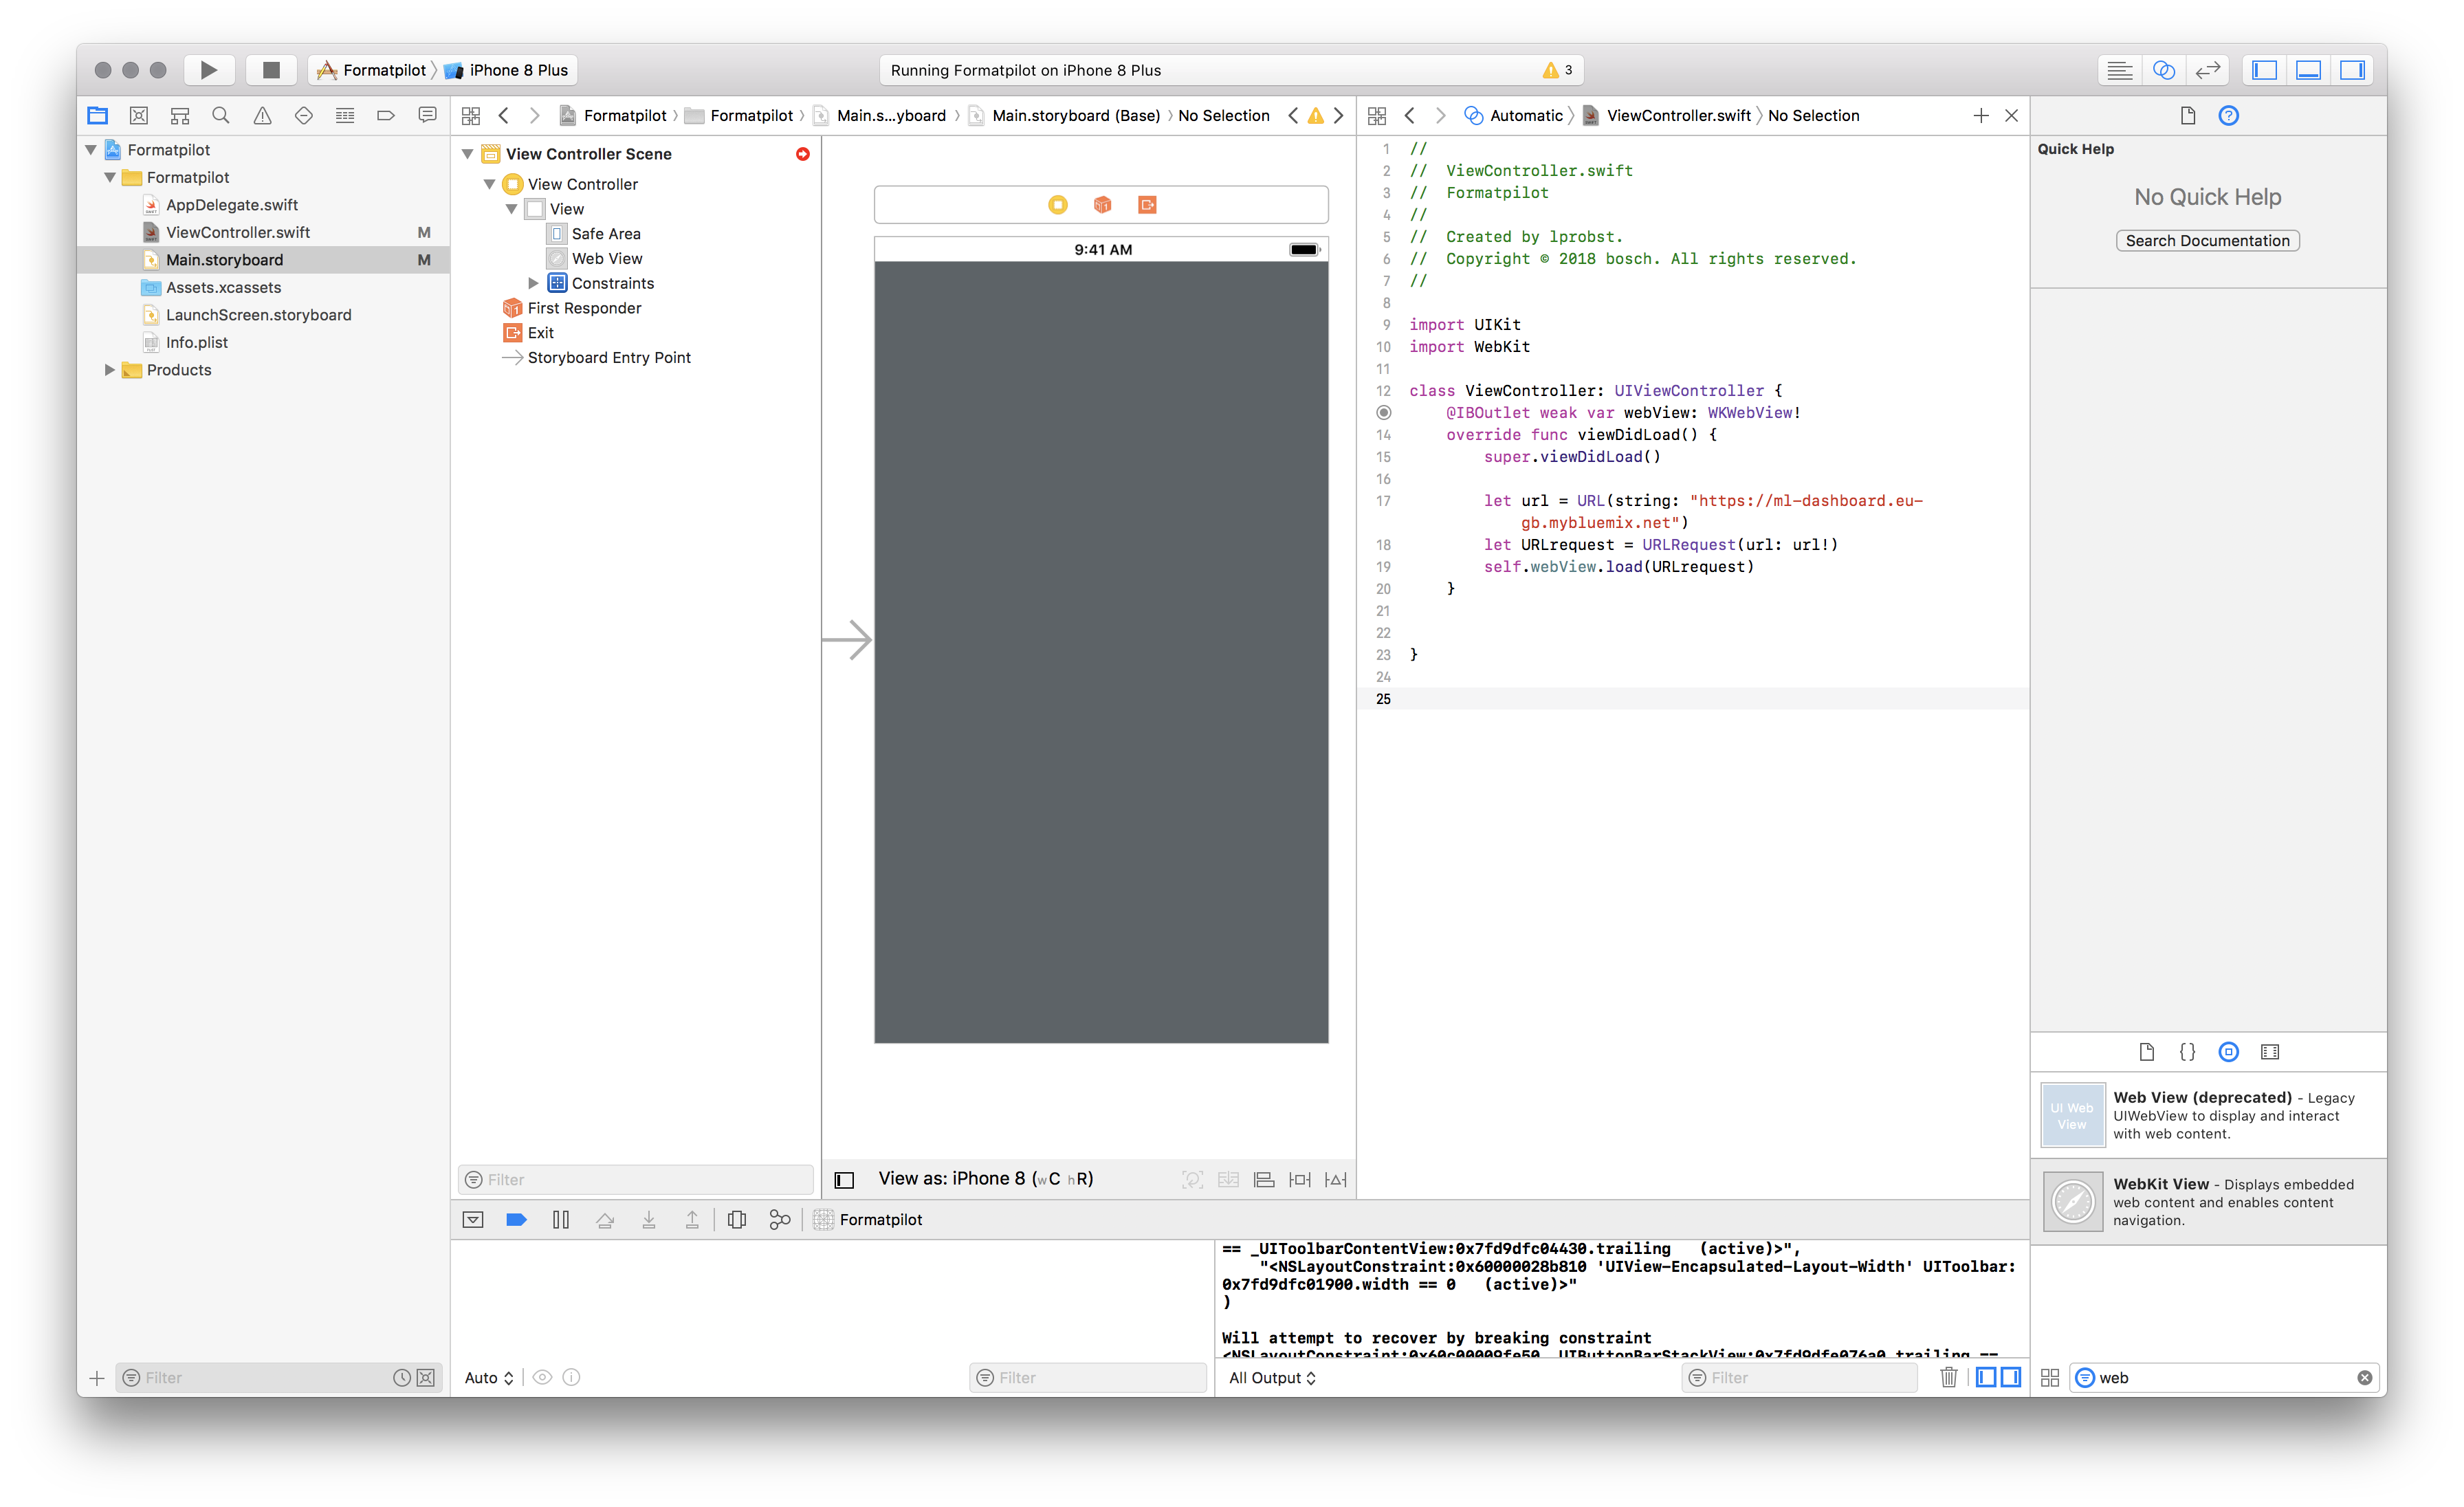
\includegraphics[width=\textwidth]{images/kapitel_4/ios_ide.png}
    \caption{Übersicht von xCode}
    \label{fig:umsetzung_ios_ide}
\end{figure}

Bei den beiden \texttt{.swift}-Dateien handelt es sich um die ausführbaren Klassen innerhalb der Anwendung. Ihn ihnen
kann man die Logik entwickeln, die für die Anwendung notwendig sind.

Dabei übergibt man in der \textit{ViewController}-Datei die genutzte View und konfiguriert diese. Wie in der Abbildung
zu sehen ist das gentzte View ein WebView-Layout, dem man die URL übergibt.

In der Datei \textit{AppDelegate} definiert man den Lifecycle der Anwendung. So kann man dort zum Beispiel festlegen,
dass der genutzte Controller das \textit{LaunchScreen}-Storyboard zugeteilt bekommt.

Generell sind die \texttt{.storyboard}-Dateien für die Darstellung der einzelnen Seiten und Menüpunkte zuständig. Davon
benötigt man lediglich eine, welche das Web-Frontend darstellt.

Zum Schluss benötigt man die \texttt{.plist}-Datei, die die Konfiguration der Anwendung übernimmt. Sie ist ähnlich der
Android-Manifest-Datei.

In der Abbildung~\ref{fig:umsetzung_ios_folder} auf Seite~\pageref{fig:umsetzung_ios_folder} ist die Übersicht der
Ordnerstruktur in xCode bgebildet. Dort sind alle benötigten Dateien zu sehen.

\begin{figure}[h]
    \centering
    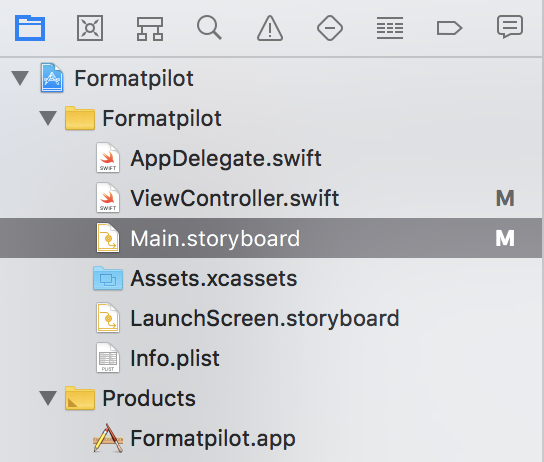
\includegraphics[scale=0.6]{images/kapitel_4/ios_folder.png}
    \caption{Ordner und Dateien in xCode}
    \label{fig:umsetzung_ios_folder}
\end{figure}

Die Plist-Datei (Property List Files) beinhaltet die Konfiguration der Anwendung. So kann man hier zum Beispiel
einstellen, ab welcher iOS-Version die App zur Verfügung steht oder ob es beispielsweise einschränkungen in der
Ausrichtung des Bildschirmes gibt. Außerdem definiert man hier den Namen der Anwendung und das verwendete Icon.

Anschließend muss man im Storyboard, also der View, ein WebView-Layout anlegen. Dies kann man mit der Programmiersprache
Swift dann ansprechen und konfigurieren. Ähnlich der Android-App kann man Informationen wie Domain oder Anzeigegröße
übergeben und das Layout kümmert sich selbstständig um das Laden, das Darstellen und die Interaktion mit dem Nutzer der
Webseite.

Mit einem Klick auf \texttt{Run} (der kleine schwarze Play-Button) in xCode, kann man den zu nutzenden Emulator
auswählen, welcher die Anwendung starten soll. In der Abbildung~\ref{fig:umsetzung_ios_app} auf
Seite~\pageref{fig:umsetzung_ios_app} ist die Anwendung im Smartphone Emulator mit der neuesten iOS Version zu sehen.

\begin{figure}[h]
    \centering
    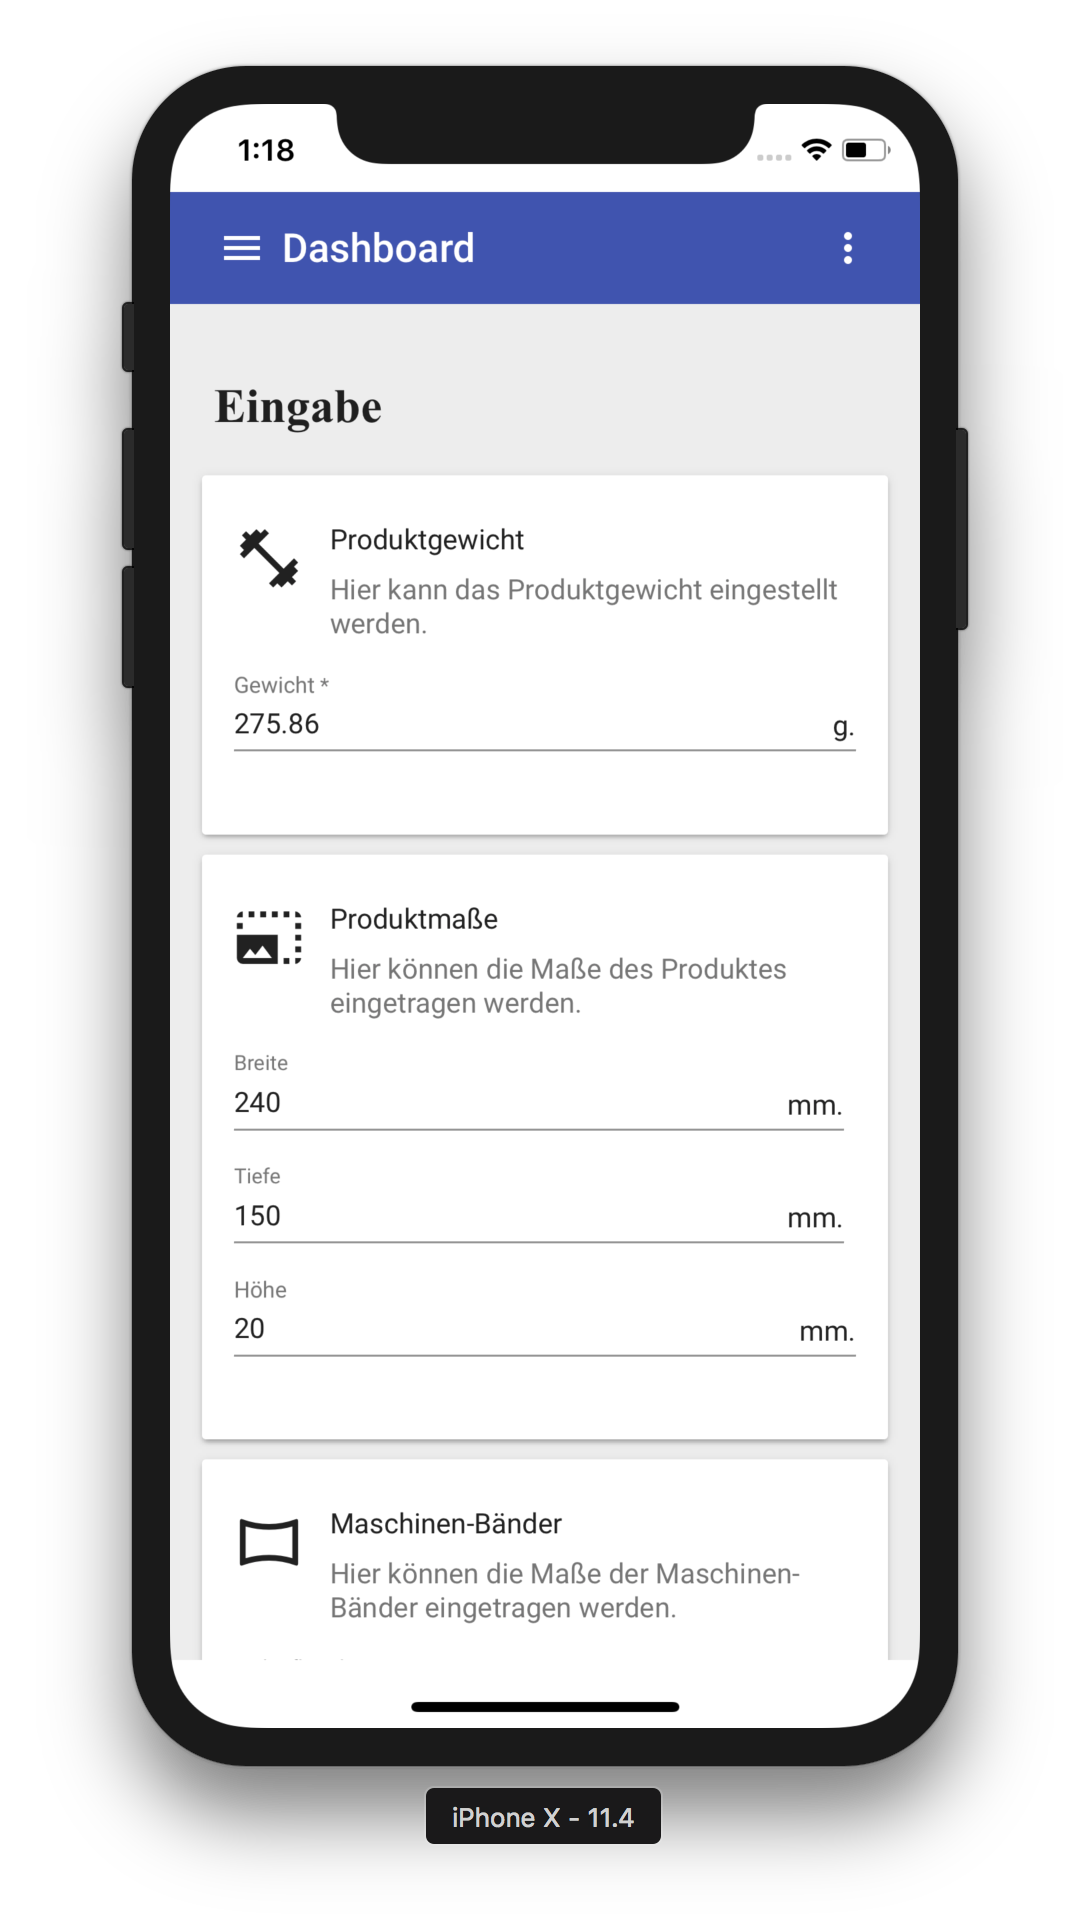
\includegraphics[scale=0.35]{images/kapitel_4/ios_app.png}
    \caption{iOS-App im Smartphone-Emulator}
    \label{fig:umsetzung_ios_app}
\end{figure}
\section{Abschluss}
So wir sind nun fertig. Man kann es auch schon nutzen. Was hat das nun gebracht? Wie sieht die fertige Architektur aus?

Überleitung zu den Alternativen. Man will das ja nachbauen können nicht nur mit der einen Maschine.

\colorbox{yellow}{Hier fehlt was}
\chapter{Adaptierbarkeit}
\label{ch:adaptierbarkeit}
Die in Kapitel~\ref{ch:neuronalesNetz} ab Seite~\pageref{ch:neuronalesNetz} aufgebaute und erstellte Architektur soll
zusammen mit dem in Kapitel~\ref{ch:client} ab Seite~\pageref{ch:client} implementierten Frontend durch weitere Ideen
erweitert und verbessert werden.

Eine Untersuchung soll ergeben, ob sowohl die Architektur als auch das Frontend so modular entwickelt wurden, dass sie 
problemlos durch weitere Funktionen und Ideen erweitert werden können. Eventuell Probleme im System oder in der
Architektur sollen gelößt werden.

Dies ist zwingend erforderlich um zum Beispiel eine weitere Maschine oder neue Module ebenfalls in das System zu
integrieren. Auch soll so auf neue Versionen oder neu herausgebrachte Maschinen reagieren werden.

Für dieses Ziel werden in den folgenden Kapitel mehrere Ideen für passende Erweiterungen behandelt und diese Schritt für 
Schritt umgesetzt und eingebaut.

Die Abbildung~\ref{fig:schematische_architektur_5} auf Seite~\pageref{fig:schematische_architektur_5} zeigt eine
schematische Erweiterung des Systems. Dort ist sehr gut ersichtlich, dass der API Connect Service eine zentrale Rolle
in der Erweiterbarkeit einnimmt.

\begin{figure}[h]
    \centering
    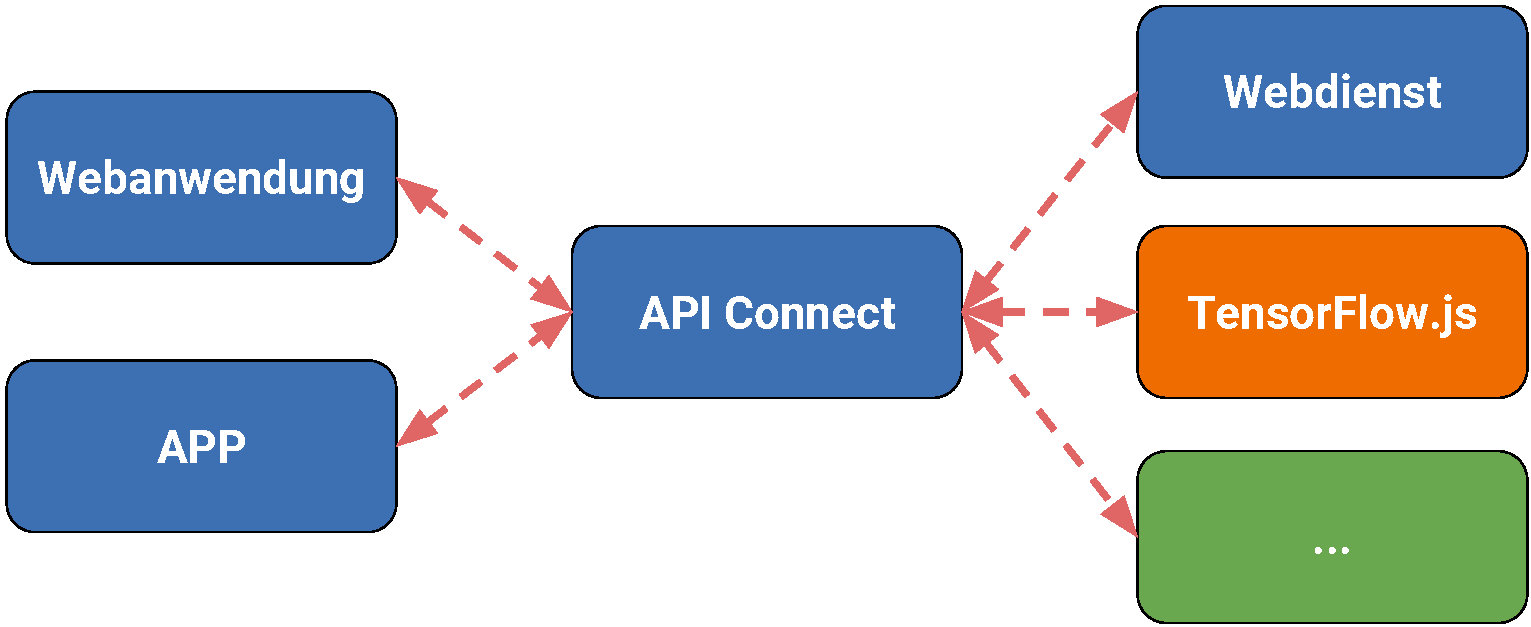
\includegraphics[width=\textwidth]{images/kapitel_5/architektur_schematisch.pdf}
    \caption{Schematische Darstellung der Adaptierbarkeit}
    \label{fig:schematische_architektur_5}
\end{figure}
\section{Schlauchbeutelmaschine}
Mit diesem Beispiel kann man die bestehende Architektur durch eine weitere Maschine ergänzen. Es ist problemlos möglich,
weitere oder andere Maschinen oder gar Module einer Maschine einzubinden. Allerdings soll mit diesem Beispiel die
allgemeine Vorgehensweise erläutert werden, und dieses Beispiel veranschaulicht dies.

In Abbildung~\ref{fig:siegelmaschinen_vffs} auf Seite~\pageref{fig:siegelmaschinen_vffs} ist der schematische Aufbau der
vertikalen Schlauchbeutelmaschine abgebildet.

\begin{figure}[h]
    \centering
    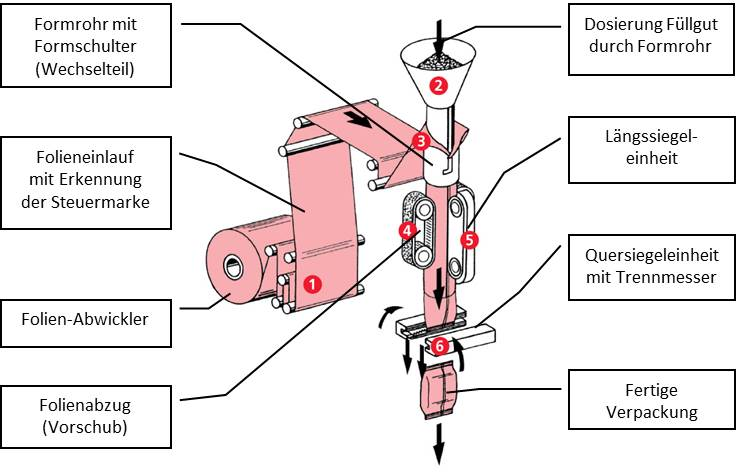
\includegraphics[scale=1]{images/kapitel_5/vffs.jpg}
    \caption{Aufbau einer vertikalen Schlauchbeutelmaschine~\cite{online_grundlagen_boschkwe}}
    \label{fig:siegelmaschinen_vffs}
\end{figure}

Dort ist gut zu sehen, dass im oberen Bereich der Abbildung, unter der Nummer 2, das zu befüllende Produkt einlegt
wird. Dies fällt dann durch das Rohr mit der Nummer 3. Eine Folie umschließt das Produkt anschließend und wird mit den
Siegelbacken (Nummer 5) versiegelt. Bei Nummer 6 trennt ein \textit{Trennmesser} den befüllten Beutel von der
Endlosfolie ab, und so kann der befüllte Beutel weiterverarbeitet werden.

Die wichtigsten Einstellparameter der Maschine betreffen die Siegelung des Beutels. Da zahlreiche Folienarten von
verschiedenen Anbietern existieren, ist es nicht immer einfach, die Folie richtig und korrekt zu versiegeln.

Die \textit{Siegelnahtfestigkeit} gibt an, welche Kraft notwendig ist, um die verschlossene Siegelnaht wieder zu öffnen.
Dies ist insbesondere dann wichtig, wenn es sich bei dem verpackten Produkt um ein Endkunden-Produkt handelt. Der Käufer
sollte die Verpackung unter normalem Kraftaufwand öffnen können, um an das Produkt gelangen zu können.

Allerdings darf die Siegelnaht nicht zu schwach sein, da sonst Luft oder andere Gase in die Verpackung eindringen
könnten. Für die vertikale Schlauchbeutelmaschine ist es entscheidend, die richtige Siegelnahtfestigkeit zu erzeugen.

Zur Erzeugung einer Siegelnaht sind Daten zur \textit{Siegeltemperatur}, \textit{Siegelzeit} und \textit{Folienart}
interessant. Bei der Folienart spielt der Aufbau der Folie (Anzahl der Lagen und genutzte Materialien) eine Rolle.

Der genaue Aufbau von Folien wird von den entsprechenden Herstellern oft geheim gehalten, und man muss ihn entweder
empirisch ermitteln oder auf Erfahrungen von Mitarbeitern zurückgreifen.

Aus diversen Tests kann man anhand der eingestellten Parameter für Siegeltemperatur und Siegelzeit und der genutzten
Folie die Siegelnahtfestigkeiten ableiten, indem man den Kraftaufwand zum Öffnen der Siegelnaht misst.

Für das weitere Beispiel ist es nun interessant, die Siegelnahtfestigkeit aus einem neuronalen Netz zu ermitteln, sofern
die Zusammensetzung der Folie sowie die Siegeltermperatur und Siegelzeit feststehen.

Ein weiteres Beispiel könnte sein, die Siegelnahtfestigkeit und genutzte Folie vorzugeben und das neuronale Netz
ermitteln zu lassen, welche Temperatur und welche Zeit für das Siegeln eingeplant werden müssen. Dieses Beispiel wird
aktuell aber nicht weiter verfolgt.

\subsection{Daten zusammenstellen}
Um an Testdaten für das Aufbauen eines neuronalen Netzes für diesen Maschinentyp zu kommen, sind zahlreiche
zeitintensive Tests und Versuche notwendig.

Für die Versuche muss man verschiedene Temperaturen mit verschiedenen Siegelzeiten und verschiedenen Folien kreuzen, was
einen enormen Zeitaufwand bedeutet.

Durch eine Zugprüfmaschine kann man anschließend die Schälfestigkeit bestimmen -- die Kraft, die bei einer schälenden
Beanspruchung aufgewendet werden muss -- um eine Naht zu öffnen. Die Prüflinge sollten dabei eine Breite von 15mm und
eine Länge 40mm aufweisen, um optimal betestet werden zu können.

Herr Felix Kruppa von der Robert Bosch GmbH hat während seiner Dissertation einen Siegelteststand aufgebaut, welcher
verschiedene Siegelnähte mit unterschiedlichen Siegelzeiten und "~temperaturen erzeugen kann.

Für den Aufbau seines Teststandes durchlief er zahlreiche Tests, welche er mit einem Protokoll dokumentierte. Diese
Daten können für die Erstellung des neuronalen Netzes fungieren, da er ebenfalls die resultierende Siegelnahtfestigkeit
ermittelte und in seiner Dokumentation festhielt.

In Abbildung~\ref{fig:siegelmaschinen_vffs_simulator} auf Seite~\pageref{fig:siegelmaschinen_vffs_simulator} ist der
aufgebaute Siegelteststand von Herrn Felix Kruppa mit Beschriftungen zu sehen.

\begin{figure}[h]
    \centering
    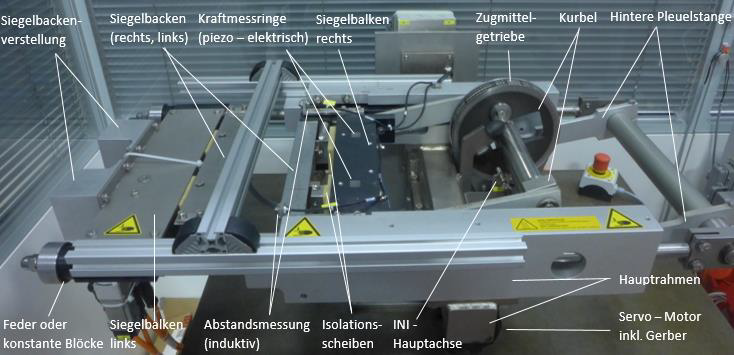
\includegraphics[width=\textwidth]{images/kapitel_5/vffs_simulator.png}
    \caption{Aufbau des Siegelteststandes}
    \label{fig:siegelmaschinen_vffs_simulator}
\end{figure}

Die kombinierten Daten aus den Testdurchläufen von Herrn Kruppa sind im Anhang~\ref{sec:schlauchbeutelmaschine}
auf Seite~\pageref{sec:schlauchbeutelmaschine} zu sehen, und man kann diese direkt für das Trainieren des neuronalen
Netzes in der Cloud oder auch offline nutzen.

\subsection{Neuronales Netz trainieren}
Mit Hilfe der zusammengestellten Testdaten kann man nun das neuronale Netz trainieren. Das Training funktioniert in
gleicher Weise wie auch in Kapitel~\ref{subsub:modeler_flow} ab Seite~\pageref{subsub:modeler_flow} mit dem Modeler
Flow in der IBM Cloud.

Dazu werden die Testdaten in den Watson Studio Service hochgeladen und anschließend mit einem Data Refinery Flow in eine
CSV-Datei umgewandelt. Der Machine Learning Service der IBM Cloud kann aktuell lediglich mit CSV-Dateien zum Trainieren
von neuronalen Netzen umgehen.

Auch kann man die Datei schon auf dem Entwicklungsrechner in eine CSV-Datei umwandeln, um sich die Konvertierung im
Service zu sparen. So muss man keinen neuen Flow für die Data Refinery anlegen. Es spielt keine Rolle, wo man die Datei
konvertiert.

Anschließend muss man einen neuen Modeler Flow anlegen und diesen genau gleich dem Flow in
Abbildung~\ref{fig:umsetzung_model_flow} auf Seite~\pageref{fig:umsetzung_model_flow} aufbauen.

In diesem Fall ändern sich aber die Parameter für die Eingabe"~ und Ausgabeparameter wie in
Tabelle~\ref{tab:targets_inputs_siegeln} auf Seite~\pageref{tab:targets_inputs_siegeln} zu sehen.

\begin{table}[h]
    \centering
    \begin{tabular}{|c|c|}
        \hline
        \textbf{Targets} & \textbf{Inputs}\\
        \hline
        \hline
        Mittelwert & Eindringverhalten\\
        \hline
        & Temperatur\\
        \hline
        & Vorwärmphase\\
        \hline
        & Eindringphase\\
        \hline
        & Siegelphase\\
        \hline
        & End-Siegel-Position\\
        \hline
    \end{tabular}
    \caption{Variablen für die Targets und die Inputs der Schlauchbeutelmaschine}
    \label{tab:targets_inputs_siegeln}
\end{table}

Nach erfolgreicher Konfiguration der einzelnen Module kann man das neuronale Netz trainieren lassen, um das Modell zu
erhalten. Dieses Modell kann man dann im Weiteren in einem Deployment zur Verfügung stellen.

\subsection{Deployment erstellen}
Um das Deployment für das trainierte Modell zu erstellen, muss man das Modell im Modeler Flow mit der rechten Maustaste
auswählen und \enquote{Save branch as a model} auswählen. Dies speichert das trainierte Modell als eigenständiges Modell
im Watson Studio ab.

Dies kann man nun über das Watson Studio Dashboard auswählen, und man kann über den Reiter \texttt{Deployments} auf alle
Webservices des einen Modells zugreifen. Dort sind aktuell aber noch keine vorhanden.

Über die Schaltfläche \texttt{Add Deployment} legt man ein neues an. Dies geschieht genau wie in
Kapitel~\ref{subsec:deployment_erstellen} ab Seite~\pageref{subsec:deployment_erstellen} beschrieben.

Nach der Eingabe eines Namens und der Speicherung des Deployments erscheint es in der anfangs leeren Liste. Damit ist
das trainierte Modell in einem Webservice zur Verfügung gestellt.

In der Abbildung~\ref{fig:siegelmaschinen_deployment} auf Seite~\pageref{fig:siegelmaschinen_deployment} ist die
komplette Konfiguration des Deployments für den Webservice ersichtlich.

\begin{figure}[h]
    \centering
    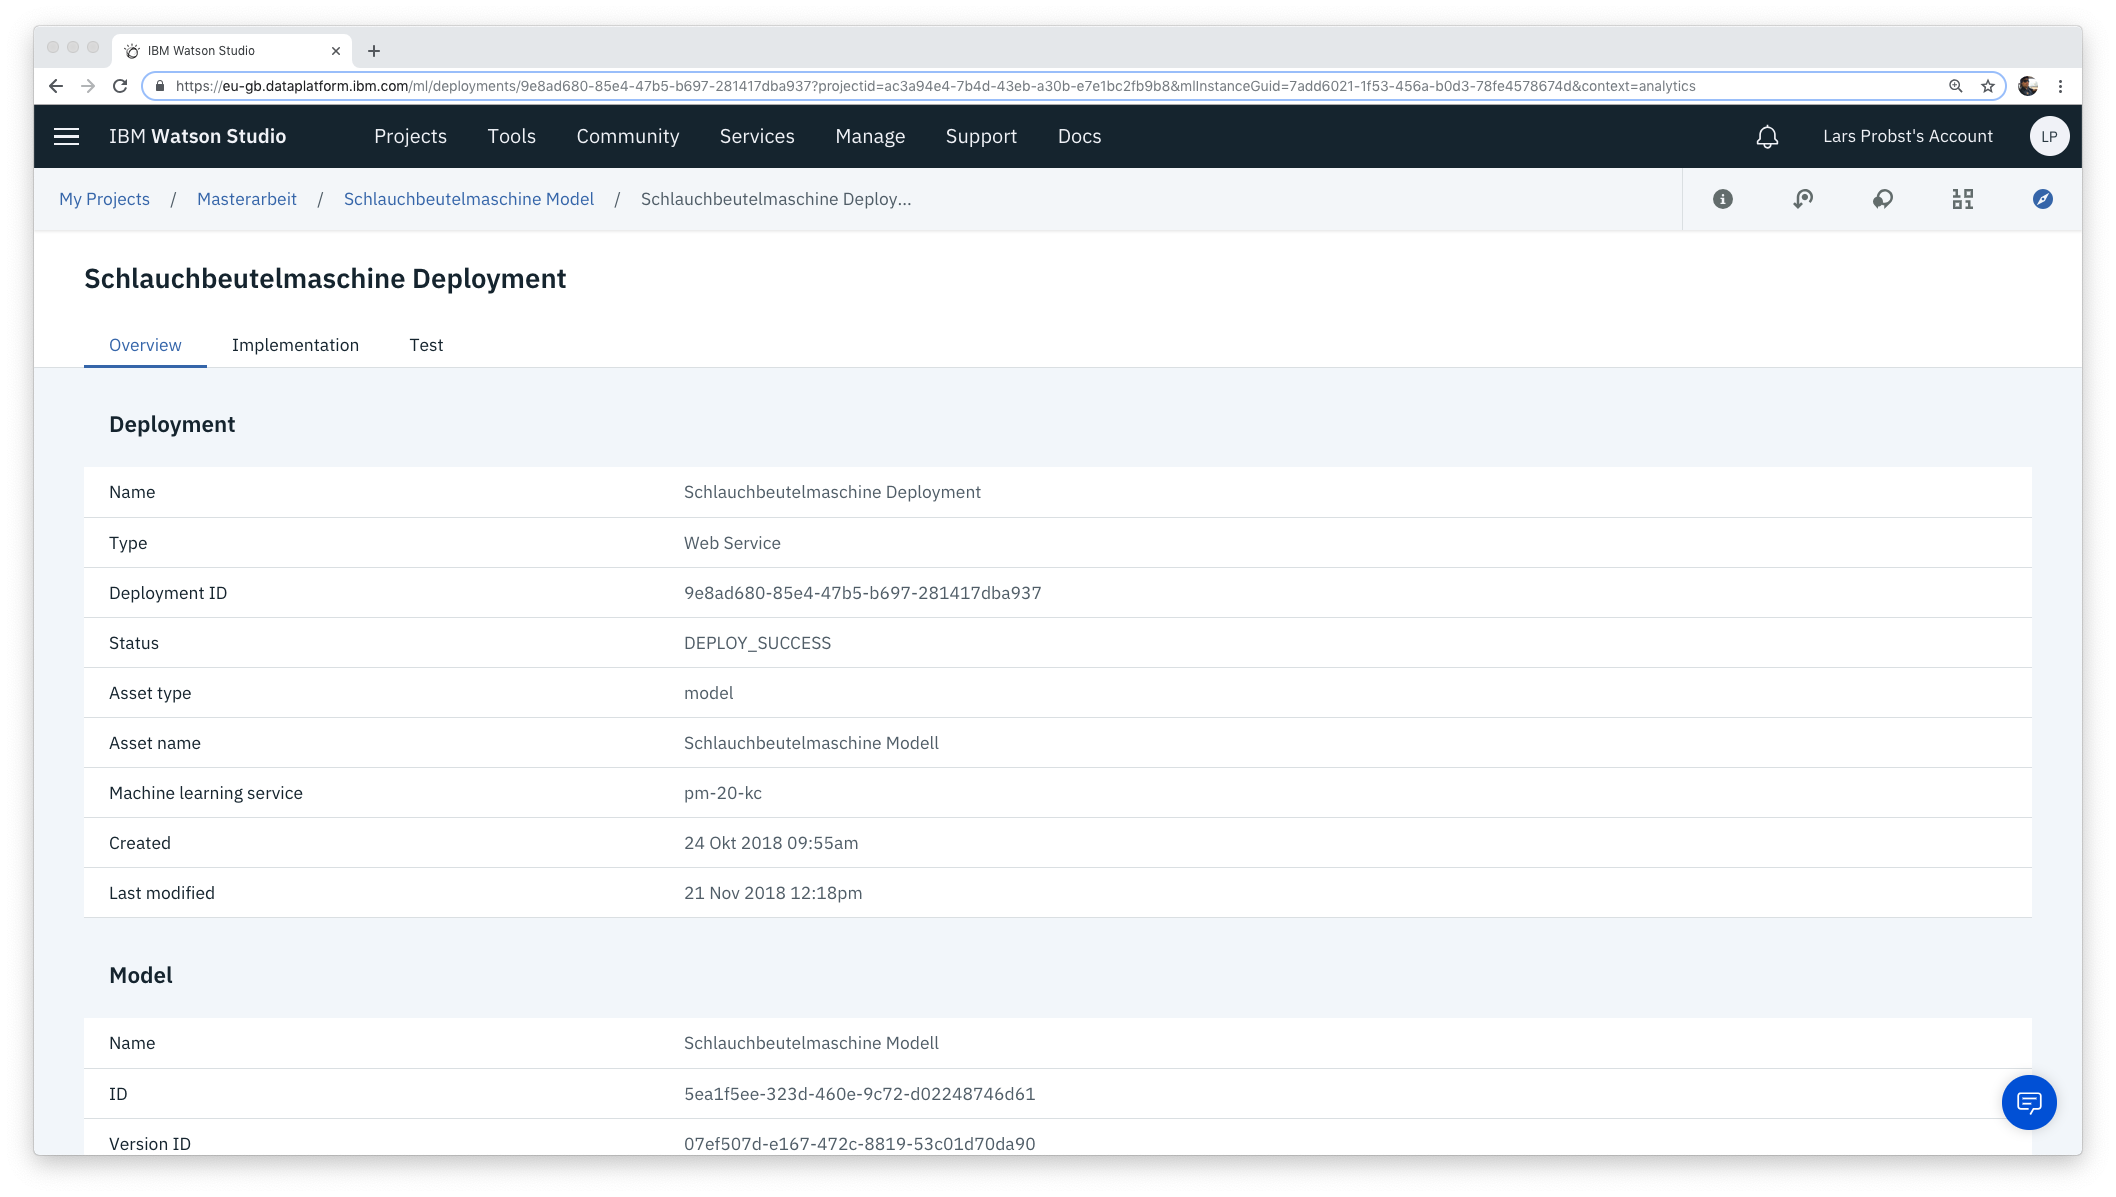
\includegraphics[width=\textwidth]{images/kapitel_5/vffs_deployment.png}
    \caption{Deployment der Schlauchbeutelmaschine}
    \label{fig:siegelmaschinen_deployment}
\end{figure}

Nun kann man in einem weiteren Schritt den API Connect Service um diesen Endpunkt erweitern, um auch Vorhersagen von
diesem neuronalen Netz zu beziehen, um die Siegelnahtfestigkeit zu ermitteln.

\subsection{API Connect erweitern}
Der API Connect Service fungiert als Knotenpunkt zwischen Frontend und den möglichen Vorhersage-Services. Damit das
Frontend auf neue Services vereinfacht zugreifen kann, muss man hier einen neuen Endpunkt anlegen. Dies kann man
entweder über die Erweiterung der JSON-Konfiguration oder über den grafischen Editor machen.

Der einfachere Weg ist die Anpassung der Endpunkt über den grafischen Editor. Damit man den neuen Service auch über den
API Service nutzen kann, muss man im Reiter \texttt{Gestalten} in der Konfiguration \texttt{Pfade} einen neuen anlegen.

Diesen kann man beliebig benennen. Ein Beispiel hierfür ist \textit{predict-seal}. Darüber hinaus muss der Pfad eine
Operation besitzen. Diese muss, genau wie alle anderen Operationen der anderen Pfade, \textit{POST} sein, damit das
Frontend Daten an den Endpunkt schicken kann.

Da der neue Pfad angelegt ist, kann man die Konfiguration speichern und in den Reiter \texttt{Assemblieren} wechseln.
Den \textit{Switch} für die Verzweigung je nach gewünschtem Pfad muss man um den gerade eingerichteten neuen Pfad
erweitern. Somit beinhaltet die Switch-Operation drei Verzweigungen.

Den Inhalt für den neuen Pfad kann man direkt vom Pfad \textit{predict-watson} übernehmen und lediglich die im
\textit{Get Prediction} Modul definierte URL für den Webservice anpassen.

Die Abbildung~\ref{fig:siegelmaschinen_apiconnect} auf Seite~\pageref{fig:siegelmaschinen_apiconnect} veranschaulicht
den angepassten Modeler Flow um den neuen Endpunkt.

\begin{figure}[h]
    \centering
    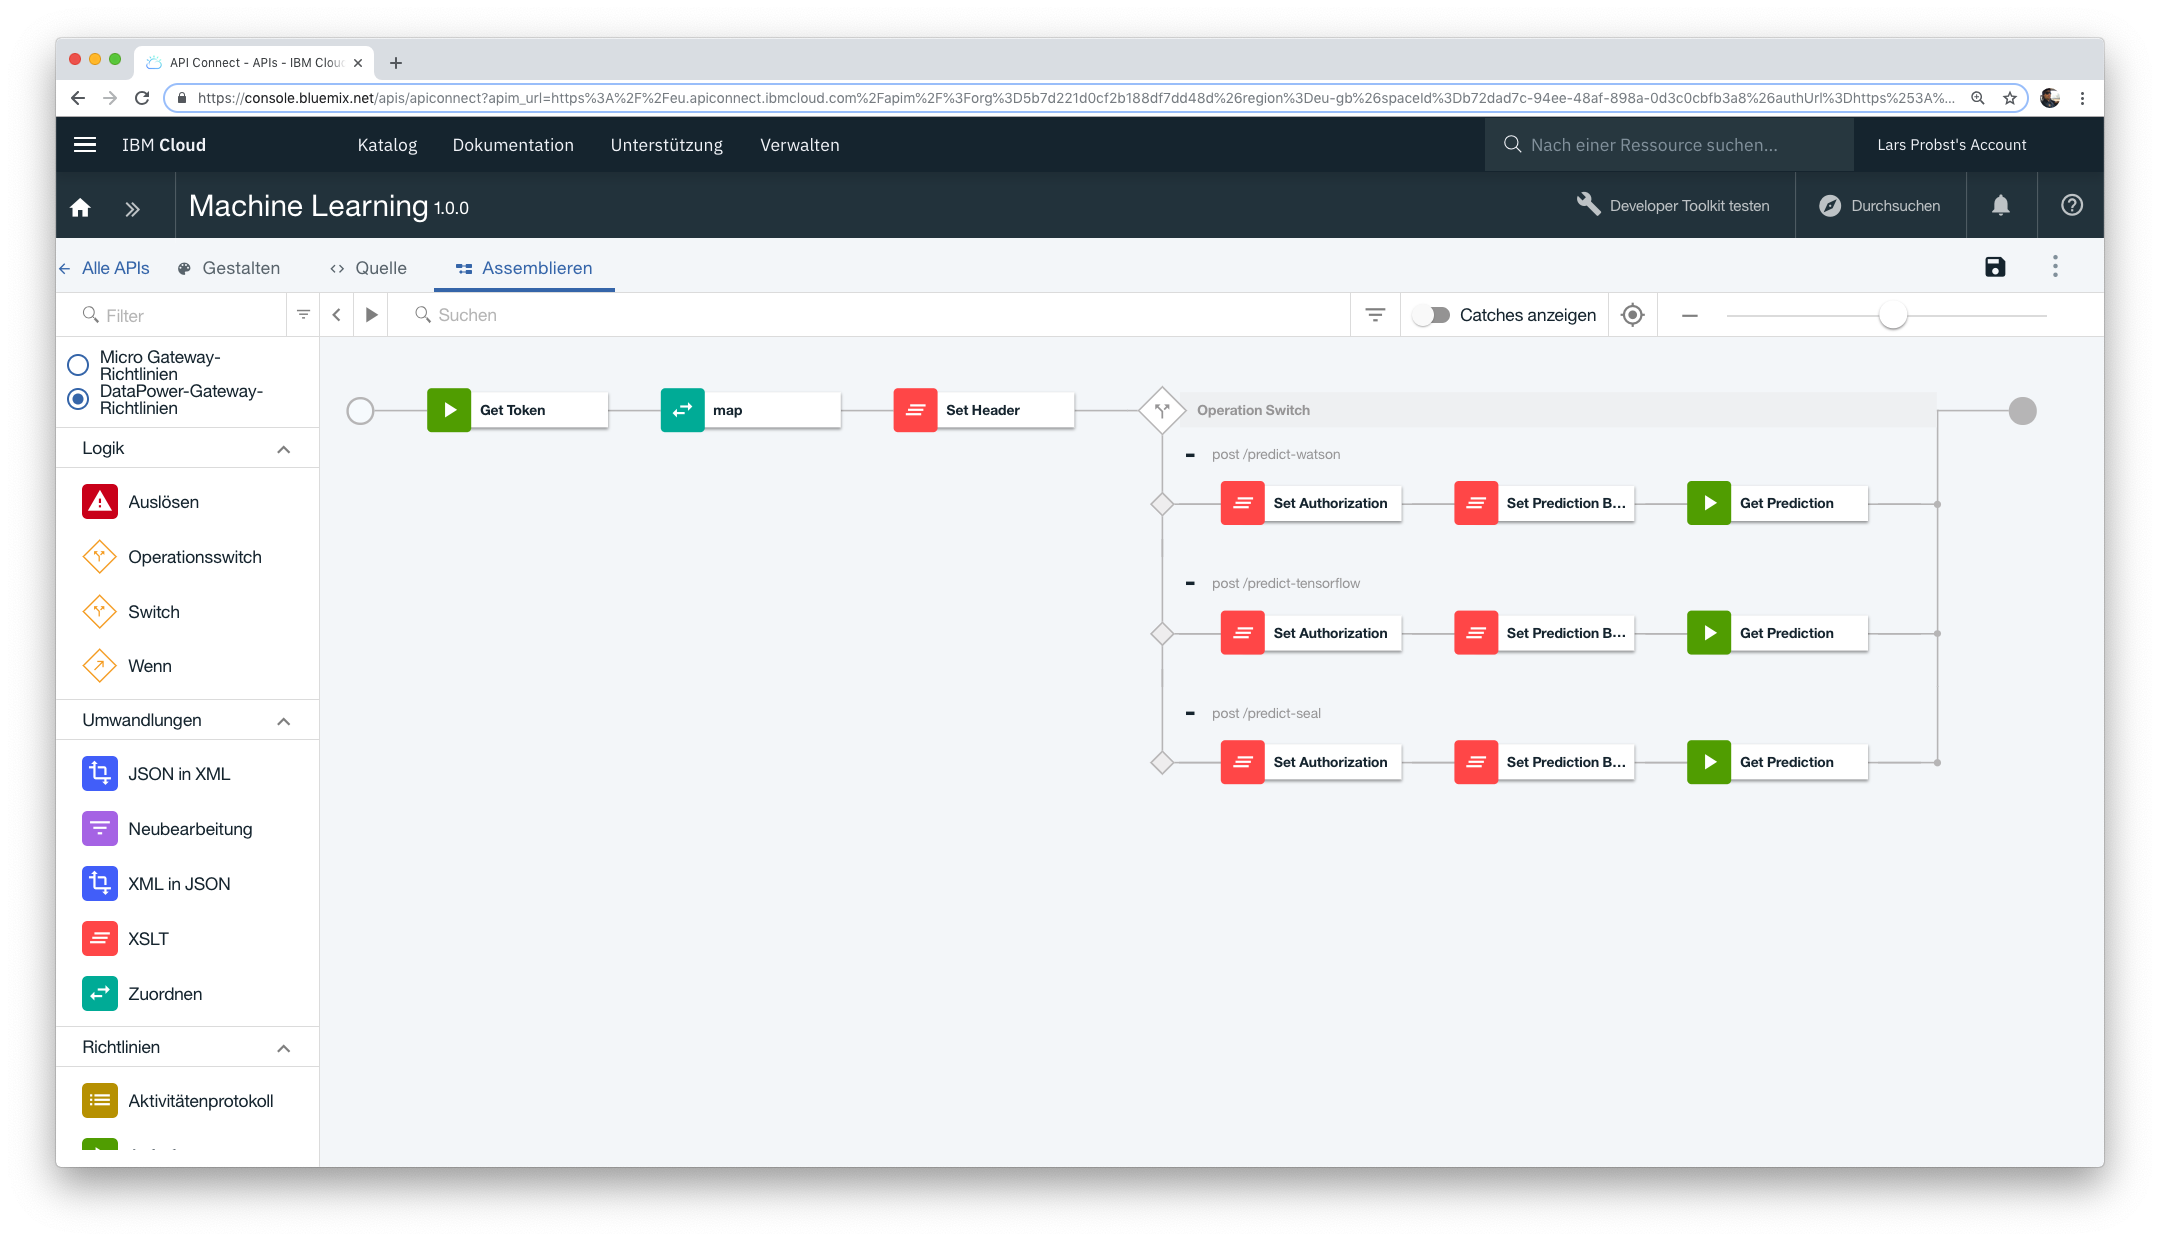
\includegraphics[width=\textwidth]{images/kapitel_5/vffs_apiconnect.png}
    \caption{Angepasster API Connect Service}
    \label{fig:siegelmaschinen_apiconnect}
\end{figure}

Damit ist der API Connect Service fertig eingerichtet, und man kann den neuen Endpunkt zum Beispiel vom Frontend aus
abrufen. Auch ist es möglich, den Aufruf mittels Postman zu überprüfen.

Ein Test mit einem externen Tool, wie zum Beispiel Postman, sollte die Funktionsweise des Endpunktes sicherstellen.

\subsection{Frontend erweitern}
Im letzten Schritt der Adaptierung der Architektur auf eine neue Maschine oder auf ein neues Modul muss man das Frontend
um die gewünschten Eingaben der Parameter erweitern, damit das Frontend die Vorhersage auf dem Webservice starten und
das Ergebnis darstellen kann.

Dafür kann man eine neue Angular-Komponente anlegen und diese dann mit dem gewünschten neuen Design versehen. Das
Anlegen einer Komponente in Angular geschieht am einfachsten über ein Kommando der Angular-CLI.

\begin{lstlisting}[caption=Erstellen einer neuen Komponente, label=ls:schlauchbeutelmaschine_component]
    ng generate component name
\end{lstlisting}

Der Parameter \textit{name} dient als Platzhalter, und man muss ihn durch einen Namen für die Komponente ersetzen. Dieser
Name darf durch keine andere Komponente vergeben sein. Die neue Komponente erscheint als Unterordner im Ordner
\texttt{app}.

Die neue Komponente besteht aus den vier Dateien \textit{*.component.css} für die Definition von CSS-Eigenschaften,
\textit{*.component.html} zur Konfiguration der Darstellung, \textit{*.component.spec.ts} für das Schreiben von Tests
und \textit{*.component.ts} für die eigentliche Logik.

Den Inhalt der vier Dateien kann man aus der Komponente für die Waage im Ordner \texttt{/app/scales} kopieren und
anschließend Stück für Stück anpassen.

In der HTML-Datei muss man das Design auf die neuen Eingabefelder abändern. Dies ist wichtig, da andere Parameter für
den Endpunkt notwendig sind.

In der TS-Datei, in der die Logik der Komponente definiert ist, muss man den REST-Endpunkt auf den neuen Namen abändern
und die übergebenen Parameter anpassen, damit die Vorhersage auch funktionieren kann.

Auch ist entscheidend, dass man die Abfrage zu leeren Feldern auf die richtige Benennung und die Definition von
zufälligen Eingabeparameter auf logische Werte anpasst. So ist es für einen Endnutzer möglich, schnell einen Test über
das Frontend zu starten.

Die CSS-Datei sowie die SPEC-Datei bedürfen keiner zwingenden Änderung, da sie für die Funktionsfähigkeit der Abfrage an
das Backend keine Rolle spielen. Allerdings sollte man zu einem späteren Zeitpunkt den Test für die Komponente
berichtigen.

\subsection{Frontend hochladen}
Als letzten Schritt muss man das überarbeitete Frontend in den Cloud Foundry Container in der Cloud laden, um es den
Endkunden zur Verfügung zu stellen.

Dafür genügt ein einfacher \textit{commit} in das lokale Git-Repository, gefolgt von einem push, um es in das Repository
in der IBM Cloud zu übertragen.

Nach wenigen Sekunden beginnt die Toolchain mit dem Herunterladen des Repositorys und dem Bau der neuen Angular-Seite.
Nach wenigen Minuten ist das aktualisierte Frontend wieder für alle über die URL aufrufbar.

Durch das Hochladen der Änderungen an dem Frontend sind auch die beiden Apps für Android und iOS mit der Aktualisierung
ausgestattet. Es ist nun auch dort möglich, Parameter für die vertikale Schlauchbeutelmaschine zu beziehen.

\subsection{Abschluss}
An diesem Punkt ist die Adaption der erstellen Architektur auf die Siegelmaschine abgeschlossen, und man kann damit
beginnen, neue Vorhersagen des neuen Webservices durch das Frontend zu beziehen. Die Ergebnisse werden anschließend
ebenfalls auf dem Frontend angezeigt.

Für alle weiteren Anpassungen oder Erweiterungen der Architektur muss man lediglich diese fünf relativ einfachen
Schritte wiederholen und die neuen Einstellungen anpassen.

Damit ist gezeigt, dass die Architektur so modular gestaltet ist, dass sie problemlos Erweiterbar und mit neuen
Funktionen ausgestattet werden kann. Dies galt es als Teilaufgabe in der Arbeit zu zeigen und beweisen.

\chapter{Ausblick}
\label{ch:ausblick}
Dieses Kapitel soll einen Überblick über weitere größere Funktionen und Erweiterungen geben, durch die die Architektur,
die Webanwendung und die Smartphone-Apps erweitert und verbessert werden können.

Außerdem sollen Möglichkeiten aufgezeigt werden, welche die Arbeit mit Maschinen und Künstlicher Intelligenz
vereinfacht. Dazu zählt unter anderem eine Möglichkeit, eine direkte Verbindung zwischen Maschine und einem trainierten
Modell herzustellen.

Auch sind Themen, welche die klassische Container-Architektur verbessern für Erweiterungen interessant oder
Möglichkeiten zur schnelleren Vorhersage von Daten und der Eingabe von Daten unter erschwerten Bedingungen.

\section{Kontinuierliches Lernen und Optimieren}
Zu Anfang sollte eine Erweiterung aufgezeigt werden, welche die Möglichkeit bietet eine Maschine direkt mit einem
neuronalen Netz und einem trainierten Modell zu verbinden, um die Maschine schneller und ohne menschlichen Einfluss
einzustellen.

In der aktuellen Version der Architektur werden neuronale Netze auf der Basis von historischen Daten aufgebaut. Die so
trainierten Modelle werden in einem Deployment zur Verfügung gestellt und können ab dann Vorhersagen bearbeiten.

Einfacher wäre es, wenn eine Maschine eine direkte Verbindung zu einem neuronalen Netz hätte und diesem kontinuierliches
aktuelle Werte übergibt, mit denen zum Beispiel die Geschwindigkeit ermittelt werden kann mit der die Maschine arbeitet
oder wie viele korrekt bearbeitet wurden -- also die bearbeiteten Produkte abzüglich dem fehlerhaften Ausschuss.

Dies wäre möglich, indem man die Maschine mit einem IoT-Gateway ausstattet, welches verschiedenste Messgrößen aus der
Maschine extrahiert und mittels MQTT an die IBM Cloud schickt. Diese Daten könnte man dann auswerten, zusammenfassen
und dem Machine Learning Service als Stream zur Verfügung stellen.

In einem Modeler Flow kann man diesen Stream dann aufgreifen und ein neues Modell kontinuierlich trainieren, sodass sich
das Modell immer neuen Gegebenheiten anpassen kann. Die Vorhersagen, die das trainierte Modell dann ausgibt, basieren
dann auf den immer neuen Maschinenparametern.

Die Cloudant-Datenbank dient als Zwischenspeicher für die immer neuen Maschinenparameter, damit diese auch für
zukünftige Auswertungen bereitstehen. Als IoT-Gateway könnte das Bsoch eigene \textit{Rexroth IoT Device} dienen.

Die \textit{Internet of Things Plattform} kümmert sich um die Verbindung zum IoT-Gateway und die Übertragung der Daten
von der Maschine auf die Cloudant Datenbank.

Die Abbildung~\ref{fig:ausblick_uebersicht} auf Seite~\pageref{fig:ausblick_uebersicht} zeigt eine Übersicht über eine
Möglichen Architektur zur automatisierten Einstellung von Maschinenparametern.

\begin{figure}[h]
    \centering
    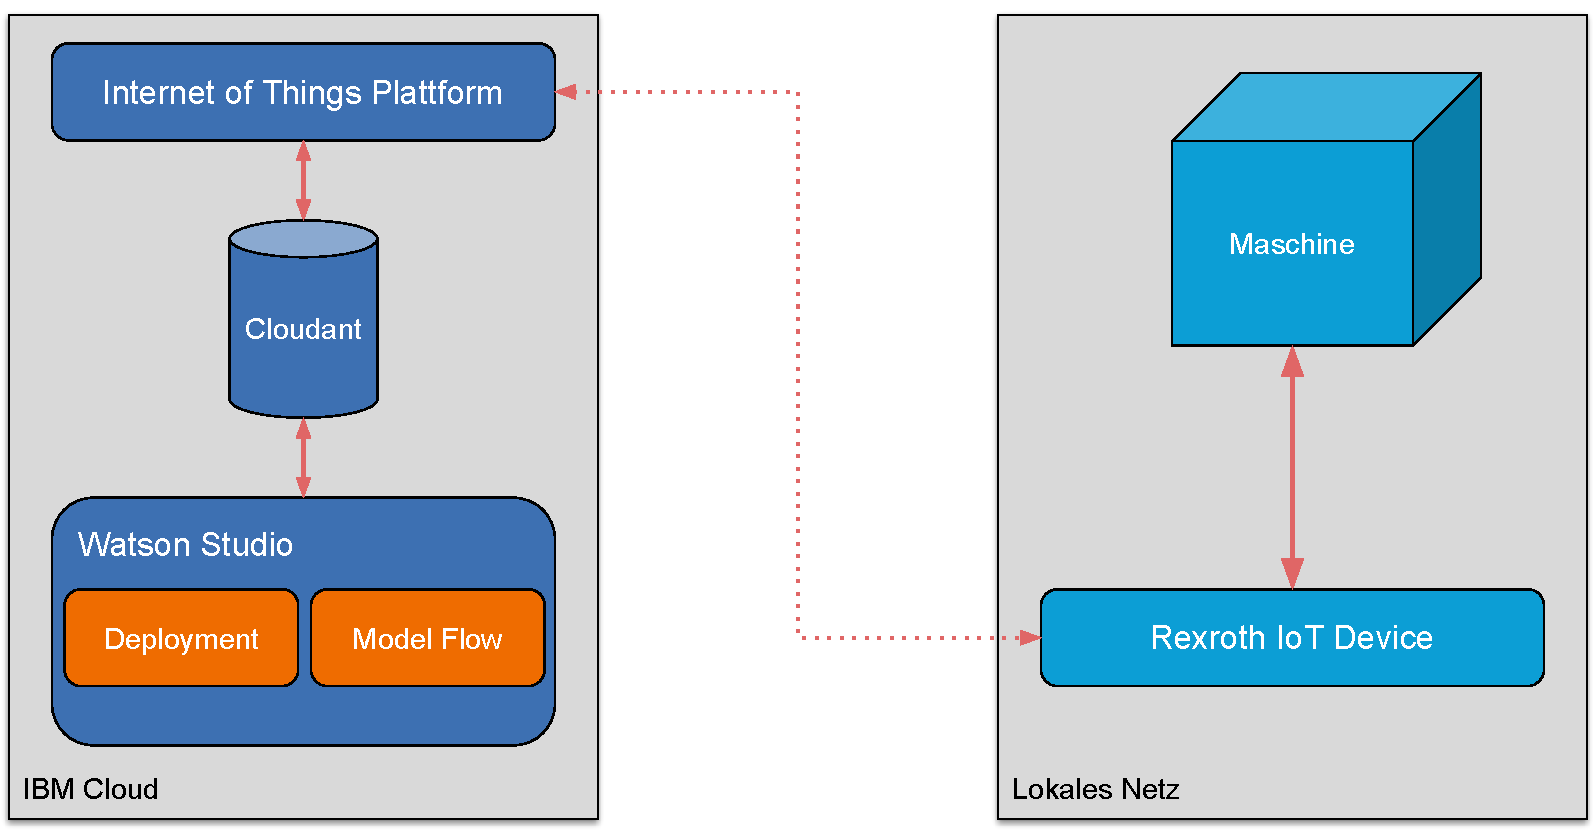
\includegraphics[width=\textwidth]{images/kapitel_6/architektur_uebersicht.pdf}
    \caption{Übersicht der Zielarchitektur}
    \label{fig:ausblick_uebersicht}
\end{figure}

Allerdings sind automatisierte Tests nicht immer und für jede Anwendung geeignet. Michael Lüttel von der Deutschen
Flugsicherung sagte auf der iqnite-Konferenz in Düsseldorf \enquote{Automatisierung macht nur dann Sinn, wenn sie mehr
Aufwände einspart als sie selbst erzeugt.}\footnote{https://www.qz-online.de/news/uebersicht/nachrichten/vor-und-nachteile-von-automatisierten-software-tests-890130.html}.

%% TODO noch schreiben
\section{Function as a Service}
Wie könnte man Functions/Lambda einbauen. FaaS

\colorbox{yellow}{Hier fehlt was}

%% TODO noch schreiben
\section{Machine Learning für Smartphones}
Wie könnte man das Feature nutzen und was würde das bringen

\colorbox{yellow}{Hier fehlt was}

%% TODO noch schreiben
\section{Offline Modus}
Ein Offline-Mode für die Website mit TensorFlow.js.

\colorbox{yellow}{Hier fehlt was}

%% TODO noch schreiben
\section{AI OpenScale}
\label{ai_openscale}
Hiermit kann man veranschaulichen, warum und wie die AI auf das Ergebnis gekommen ist. Das kann man mit dem Deployment
und mit dem TensorFlow.js Ding machen. Dafür braucht man eine Datenbank.

\colorbox{yellow}{Hier fehlt was}

%% TODO nosch schreiben
\section{Skalierbarkeit}
Wie könnte man die Anwendung skalieren?

\colorbox{yellow}{Hier fehlt was}

%% TODO noch schreiben
\section{Audit mit Blockchain}
Für die Waage muss Audit gemacht werden. Könnte man Blockchian da nicht noch einbauen?

\colorbox{yellow}{Hier fehlt was}

%% TODO noch schreiben
\section{Nutzen von IoT}
Nutzen von IoT

\colorbox{yellow}{Hier fehlt was}

\begin{figure}[h]
    \centering
    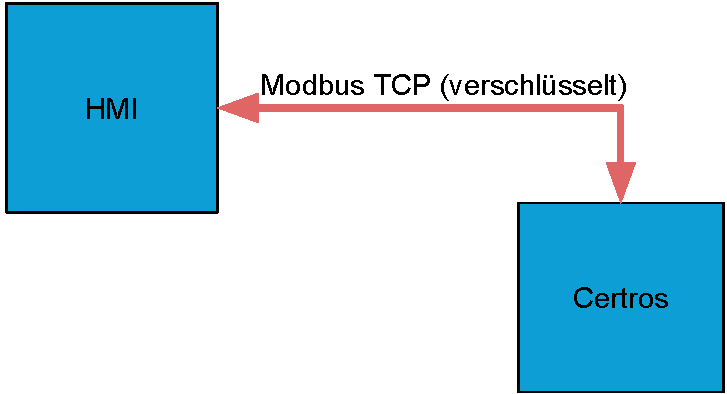
\includegraphics[width=\textwidth]{images/kapitel_6/iot_waage.pdf}
    \caption{Übersicht der Zielarchitektur}
    \label{fig:ausblick_iot}
\end{figure}

%% TODO noch schreiben
\subsection{Daten einlesen}
Wie könnten die Daten, welche durch das Netzwerk herausgefunden werden, auch automatisch in die Machine eingegeben werden?

\colorbox{yellow}{Hier fehlt was}

%% TODO noch schreiben
\subsection{Daten auslesen}
Wie könnte man Daten der Maschine auslesen, damit man sie nutzen kann um das Neuronale Netz weiter zu verbessern?

\colorbox{yellow}{Hier fehlt was}
\chapter{Zusammenfassung}
\label{ch:zusammenfassung}
Im Rahmen dieser Arbeit wurde ein neuronales Netz auf Basis von historischen Daten trainiert, welches der Robert Bosch
GmbH dabei hilft, die produzierten Verpackungsmaschinen schneller an den Endkunden auszuliefern, indem die
einzustellenden Formatparameter der Maschine durch präzise Vorhersagen und nicht durch langes Testen eines Mitarbeiters
ermittelt werden können.

Gerade durch die Modularität der erstellten Architektur können Vorhersagen auch für weitere Maschinen erfolgen. Dabei
können Teile der Anwendung sowohl in einer beliebigen Cloud als auch im eigenen Rechenzentrum laufen, ohne größeren
Entwicklungsaufwand bei der Umstellung zu generieren.

Die Basis für die Anwendung bildet das neuronale Netz sowie das darauf trainierte Modell, welches in Echtzeit
Vorhersagen tätigen kann und über mehrere Schnittstellen erreichbar ist.

Zum Start der Arbeit wurden historischen Daten gesammelt, um darauf anschließend ein neuronales Netz zu trainieren. Das
daraufhin erstellte Deployment des Modells mit eigener Schnittstelle erfolgte automatisiert aus der Cloud heraus.

Zusätzlich ist das extrahierte Modell in einem TensorFlow-Wrapper nutzbar, um es unabhängig von einer Cloud zu
betreiben. Auch konnte so getestet werden, ob Vorhersagen für gleichen Parameter in unterschiedlichen Deployments
übereinstimmen.

Ein Cloud Service für die Bündelung der Anfragen an die beiden Endpunkte ist in einem weiteren Schritt eingerichtet
worden. Über diesen ist es möglich, die Anfragen der Frontends zu normieren und Benutzerdaten des Watson Deployments zu
verschleiern.

Abschließend bleibt mir zu sagen, dass ich die in der Einleitung erwähnte Aussage von Amy Webb insoweit unterstütze,
dass mit künstlicher Intelligenz viele neue Möglichkeiten zur Lösung von aktuellen und zukünftigen Problemen entstehen.

Laut einer aktuellen IDC-Studie~\cite{article_zusammenfassung_idc} arbeiten und beschäftigen sich mehr als 50\% der
deutschen Unternehmen mit künstlichen Intelligenz. Allerdings bremst auch hier \enquote{Der Fachkräftemangel (\ldots)
den Fortschritt vieler Unternehmen aus.}.


% Alle Einträge der BibTeX Datenbank zitieren
\nocite{*}

% Einstellen des Bibliography-Stils für das Literaturverzeichnis
\bibliographystyle{abbrvdin}

% Auswahl der BibTeX Datenbank für das Literaturverzeichnis
\bibliography{literatur}

% Abbildungsverzeichnis ausgeben
\listoffigures

% Tabellenverzeichnis ausgeben
\listoftables

% Das Listings-Verzeichnis scheint mit manchen Versionen vom Koma-Script
% bzw. des Listings Pakets nicht ohne weiteres zu funktionieren
\lstlistoflistings

% Anhang beginnen (Formatierung umschalten)
\appendix
\chapter{Anhang}
\label{ch:anhang}

%% TODO noch hinzufügen
\section{Konfiguration des API Connect Services}
\label{sec:konfigurationAPIConnect}
\colorbox{yellow}{Hier fehlt was}

\section{Datensatz der KWE Waage}
\label{sec:scaleData}
Die größe des Dokuments und die Anzahl der Zeilen und Spalten würde den hiesigen Platz sprengen. Desshalb liegt das
Dokument auf der beigelegten CD mit dem Namen \texttt{datensatz\_kwe.xlsx} bereit.

\section{Datensatz der Siegelmaschine}
\label{sec:hariboSiegel}
Die größe des Dokuments und die Anzahl der Zeilen und Spalten würde den hiesigen Platz sprengen. Desshalb liegt das
Dokument auf der beigelegten CD mit dem Namen \texttt{datensatz\_siegelmaschine.xlsx} bereit.

\newpage

\section{Postman Testparameter}
\label{sec:postmanTestparameter}

\begin{lstlisting}[language=JSON, caption=Testparameter für Postman, label=ls:anhang_postman, escapeinside=``]
    {   "fields": [
            "Einlaufbandl`\textcolor{blue}{ä}`nge",
            "W`\textcolor{blue}{ä}`gebandl`\textcolor{blue}{ä}`nge",
            "Auslaufbandl`\textcolor{blue}{ä}`nge",
            "Einlaufbandbreite",
            "W`\textcolor{blue}{ä}`gebandbreite",
            "Auslaufbandbreite",
            "Einlaufbandrolle",
            "W`\textcolor{blue}{ä}`gebandrolle",
            "Auslaufbandrolle",
            "Produktbreite",
            "Produktl`\textcolor{blue}{ä}`nge",
            "Produkth`\textcolor{blue}{ö}`he",
            "Leistung",
            "Packungsgewicht",
            "Bandgeschwindigkeit",
            "Position",
            "Totzeit",
            "Impuls",
            "Druckluft"
        ],
        "values": [
            [
                415,
                360,
                470,
                250,
                250,
                250,
                29,
                29,
                29,
                240,
                150,
                20,
                220,
                275.86,
                null,
                null,
                null,
                null,
                null
            ]
        ]}
\end{lstlisting}

\newpage

\section{Konfiguration des Service Worker}
\label{sec:serviceWorkerConfig}

\begin{lstlisting}[language=JSON, caption=Konfiguration des Service Workers, label=ls:anhang_serviceworker]
    {
        "index": "/index.html",
        "assetGroups": [
            {
                "name": "app",
                "installMode": "prefetch",
                "updateMode": "prefetch",
                "resources": {
                    "files": [
                        "/favicon.ico",
                        "/index.html",
                        "/*.css",
                        "/*.js"
                    ]
                }
            },
            {
                "name": "assets",
                "installMode": "prefetch",
                "updateMode": "prefetch",
                "resources": {
                    "files": [
                        "/assets/**"
                    ]
                }
            },
            {
                "name": "fonts",
                "installMode": "lazy",
                "updateMode": "lazy",
                "resources": {
                    "urls": [
                        "https://fonts.googleapis.com/**",
                        "https://fonts.gstatic.com/**"
                    ]
                }
            }
        ]
    }
\end{lstlisting}

% Ausgabe des Wortindex
%\clearpage
%\addcontentsline{toc}{chapter}{Index}
%\printindex

\end{document}
